\def\CCluster#1{\rm{C_{#1}}}
\chapter{石墨烯的生长机理研究}
\label{cap:石墨烯的生长机理研究}
\section{引言}
如今,化学气相沉积法已经成为大规模石墨烯生长的主要合成方法。以铜为代表的金属衬底对含碳前驱体的催化作用极大提升了石墨烯的产率。同时,铜衬底自限制效应及较低的碳溶解度抑制了多层石墨烯的生长,提升了石墨烯单层性。尽管如此,由于石墨烯在化学气相沉积法进行生长的过程中通常为多点成核同时生长的方式,所以尽管在铜衬底的表面可以实现单层石墨烯生长,但生长而成的石墨烯通常为多晶的形式,各石墨烯晶畴之间由于生长取向的不同存在晶界。而要实现大面积单层石墨烯单晶的生长,则需要尽可能地扩大单个石墨烯晶畴的面积、尽可能地消除晶界。目前,化学气相沉积法实现大面积石墨烯单晶生长的方式主要有两种。一种是对石墨烯的成核数量进行限制。通过在衬底上实现单点成核,将单晶畴石墨烯缓慢长大的方式实现大面积的单晶石墨烯薄膜。另一种方式是对石墨烯的生长晶向进行调控。通过将多个晶向相同的石墨烯晶畴融合的方式,尽可能地消除石墨烯晶畴之间的晶界,使其能够尽可能完美的形成单晶石墨烯薄膜。相比于限制成核的方式,控制石墨烯生长晶向,使得多点成核的石墨烯畴同时同向生长,更容易实现石墨烯单晶的大规模制备。%//TODO 引用

由于铜衬底与碳原子较弱的相互作用,石墨烯在铜衬底上的生长方式主要遵循扩散生长机制。在扩散生长机制的作用下,含碳前驱体在铜衬底表面裂解形成具有活性的碳原子,碳原子在铜衬底表面扩散成核生长形成石墨烯晶畴。可以认为,石墨烯的生长过程主要发生在铜衬底的表面,因此理解石墨烯生长过程中和铜衬底表面的作用是理解石墨烯生长机理以及控制石墨烯生长晶向的关键。同时,已有研究表明,在氢原子不足的情况下,石墨烯晶畴边缘的碳原子能够与铜衬底成键。边缘碳与铜衬底的作用会导致石墨烯畴在成核生长的过程中倾向于某些特定的角度,而且高指数晶面所产生的台阶可能会进一步增强这种角度限制作用\citing{RN694-2019, RN693-2014}。%//TODO 引用

在\ref{sec:石墨烯优先生长取向}章中,我们使用密度泛函理论,计算了石墨烯在铜衬底表面存在台阶时的优先生长取向。计算结果证明,衬底表面的台阶破坏了原衬底表面的对称性,为石墨烯的成核生长提供了优先生长位点,同时使得石墨烯晶畴的优势生长角度由原来在平坦衬底上非重叠的$\SI{\pm 18}{\degree}$ 、 $\SI{\pm 15}{\degree}$坍缩至铜衬底台阶边缘的$\SI{\pm 0}{\degree}$ 或者 $\SI{\pm 30}{\degree}$,石墨烯晶畴展现出倾向于单一方向的成核生长。

在大面积石墨烯单晶生长的基础上,我们希望能够在化学气相沉积生长的过程中对石墨烯的层数做进一步的调控。作为一种二维材料,对石墨烯的层数和堆叠方式进行控制可以改变石墨烯的电子结构、光电性质,使其能够更好的在电子、光电子器件中发挥作用\citing{RN1068-2020, RN1100-2021, RN1071-2021, RN1065-2013, RN1067-2020, RN854-2020, RN1066-2015, RN855-2018}。
虽然铜衬底自限制效应及较低的碳溶解度,极大地提升了石墨烯单层性,但也带来了石墨烯生长过程中层数调控的困难\citing{RN1102-2013, RN1081-2019, RN1080-2015} 。目前,已有许多研究者利用各种方法实现了双层或者是少层石墨烯的生长。这些非单层石墨烯的生长机制基本上可以分为三类,包括多层石墨烯共同生长、多层石墨烯在首层石墨烯上表面生长、多次石墨烯在首层石墨烯下表面生长。这里的上表面对应于暴露在生长环境中的石墨烯表面,而下表面则对应于和衬底向接触的石墨烯表面。%//TODO 引用

甲烷等含碳前驱体在化学气相沉积的过程中作为反应物,经过热解反应、气相化学反应、组分输运过程,在衬底的表面转化为石墨烯。通常研究者会在生长石墨烯时引入氢气,氢气和甲烷的组合可以较方便的调整石墨烯生长环境中碳源的浓度,方便对石墨烯的尺寸、形态进行控制。同时在氢气环境下甲烷裂解不会产生额外的副产物,保证了石墨烯生长碳源的纯度。氧气的引入会清除衬底表面的杂质碳,从而降低石墨烯的成核密度,提升石墨烯的晶畴大小\citing{RN1083-2016, RN1104-2013, RN1085-2016}。同时,氧气的引入会进一步改变甲烷裂解的反应过程,为衬底下方的背扩散提供额外的碳源。通过背扩散的方式进入到铜-石墨烯界面之间的碳源会在石墨烯的下表面成核\citing{RN1079-2014, RN1052-2016, RN1080-2015}。这种利用碳在衬底内的背扩散是生长多层石墨烯的一种方式,研究者还利用同位素标记、理论计算等方法证明了碳原子在石墨烯边缘侧扩散\citing{RN1102-2013, RN247-2014}以及石墨烯表面直接穿透\citing{RN248-2014}的方式都可以在石墨烯的下表面生长多层石墨烯。

在\ref{sec:石墨烯氧蚀刻穿透}章中,我们利用化学反应动力学模拟、密度泛函理论计算等方法,建立了多层石墨烯生长过程中的氧辅助蚀刻/穿透模型。在这个模型中,氧气一方面能够通过交换作用,透过第一层石墨烯蚀刻处于石墨烯-衬底界面处的石墨烯附加层。另一方面,氧气也能够辅助生长环境中的碳源,穿过石墨烯覆盖层,在石墨烯-衬底界面处进行石墨烯附加层的成核生长。我们的模型解释了氧气对石墨烯多层的蚀刻和穿透作用的相互竞争突破了原有铜衬底上石墨烯生长的自限制作用,导致了石墨烯多层交替出现蚀刻和生长的现象。

%//TODO 引言 衬底影响+氧气的影响
\section{计算细节}
%//TODO vasp 引用等
在本章中密度泛函理论主要使用Vienna ab-initio Simulation Package (VASP) 软件包进行计算。由于石墨烯畴$\CCluster{24}$与铜衬底均为非磁性体系,出于计算资源的限制,经过测试后我们在 \ref{sec:石墨烯优先生长取向} 章中均采用自旋非极化的计算设置。在密度泛函理论计算中,我们使用广义梯度近似(GGA)下的 Perdew-Burke-Ernzerhof (PBE)泛函描述电子之间的交换关联作用。平面波的截断动能取为为$\SI{400}{\electronvolt}$。为了研究铜衬底表面石墨烯的生长情况,我们采用切片模型并在垂直表面方向放置至少$\SI{20}{\angstrom}$的真空层以防止周期性条件相邻切片的影响。在原子结构优化的计算中,力收敛条件设为$\SI{2e-2}{\electronvolt \per \angstrom}$,电子结构自洽场计算的收敛条件设为$\SI{1e-6}{\electronvolt}$。

在 \ref{sec:石墨烯优先生长取向} 章中,由于切片模型较大的模拟晶胞尺寸,我们在布里渊区中取 $\Gamma$ 点作为积分采样的K空间网格。

在 \ref{sec:石墨烯氧蚀刻穿透}章中,铜衬底-石墨烯体系内的范德瓦尔斯作用使用Grimme的DFT-D2方法进行描述。不失一般性的,我们选用铜(111)面作为生长多层石墨烯的衬底。在切片模型中,衬底由至少四原子层的铜(111)面组成。由于切片模型较大的模拟晶胞尺寸,我们在布里渊区中取 $\Gamma$ 点为中心的$2\times 2\times 1$网络作为积分采样的K空间网格。

对于化学气相沉积系统中化合物组成浓度的计算,我们使用CHEMKIN软件进行稳态下的气相动力学模拟。对于化学气相沉积系统中含时浓度分布的计算,我们使用fluent软件将流体力学与气相动力学进行耦合,以模拟化学气相沉积系统的生长气氛中瞬态的组成浓度分布。甲烷-氧气-氢气之间的化学反应机制、反应参数以及输运性质由GRI-MECH 3.0反应数据库提供,模拟共涉及碳、氧、氢三个元素攻击201个元化学反应过程。反应炉设置为常见的一英寸管,直径为\SI{5.08}{\centi\metre},长度为\SI{60}{\centi\metre}。反应炉的中央\SI{40}{\centi\metre}区域为高温区,温度为\SI{1323}{\kelvin}。石墨烯的生长位置位于高温区的中央。

\section{衬底对化学气相沉积法中石墨烯生长晶向的作用}
\label{sec:石墨烯优先生长取向}
为了探究石墨烯在铜衬底表面的优先生长取向,我们使用碳团簇$\CCluster{24}$作为我们的主要研究对象,考察石墨烯成核生长过程的早期过程中铜衬底表面晶向和台阶的密度对于石墨烯生长方向的影响。对于铜衬底表面晶面结构的选取,我们选择铜(001)以及铜(111)晶面以及以二者为台面的台阶铜表面结构作为研究对象,以覆盖铜衬底表面晶面指数为$\rm{(11n)(n \geqslant 1)}$的情况。
在本章中,我们使用$E_{\rm{f}}$来表征不同生长方向的$\CCluster{24}$团簇在铜衬底表面的形成能。
\begin{equation}
    E_{\rm{f}}=
    (E_{\rm{Cu+\CCluster{24}}}-E_{\rm{Cu}}-E_{\rm{\CCluster{24}}})
\end{equation}

其中,$E_{\rm{Cu+\CCluster{24}}}$为通过第一性原理计算获得的石墨烯$\CCluster{24}$团簇吸附铜衬底上的总能量,$E_{\rm{Cu}}$为单独铜衬底的能量,$E_{\rm{\CCluster{24}}}$为单独石墨烯$\CCluster{24}$团簇的能量。

如图\ref{fig:GO_calculateFlow}所示,对于不同衬底表面上石墨烯$\CCluster{24}$团簇优先生长方向的搜索以及不同生长方向的相对能量计算,我们使用全优化的方式枚举计算不同衬底表面石墨烯$\CCluster{24}$团簇的最优和次优生长方向。为了尽可能搜寻石墨烯$\CCluster{24}$团簇在不同衬底表面的能量最低构型,我们枚举了不同的生长位点,并在每个生长位点上以$\SI{6}{\degree}$或者$\SI{3}{\degree}$的间隔枚举不同的生长方向。 确定不同衬底表面石墨烯$\CCluster{24}$团簇的最优和次优生长角度后,我们使用线性插值的方式,计算最优和次优生长方向之间的石墨烯$\CCluster{24}$团簇内部的碳原子位置作为中间态。最后,通过固定碳原子XY轴,在Z轴方向优化的方式对这些固定团簇生长角度的中间态进行结构优化,获得石墨烯$\CCluster{24}$团簇在最稳和次稳生长方向之间各个生长角度的形成能$E_{\rm{f}}$。石墨烯$\CCluster{24}$团簇的生长方向以其相对于衬底的方向进行标识。考虑到本章的主要研究对象为晶面指数为$\rm{(11n)(n \geqslant 1)}$的铜衬底。$\rm{(11n)(n \geqslant 1)}$中的高指数铜衬底可以看看成由铜(100)或者铜(111)台面与<110>晶向的台阶组合而成。因此我们使用$\CCluster{24}$团簇的锯齿边(zigzag)与铜衬底表面的<110>晶向的相对夹角$\Theta$作为$\CCluster{24}$团簇的生长方向的指标(图\ref{fig:GO_relativeAngle})。

\begin{figure}[htb]
    \subfloat[]{
        \label{fig:GO_calculateFlow}
        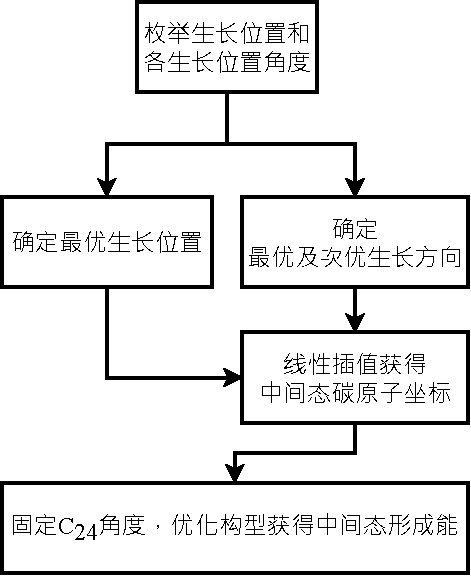
\includegraphics[width=0.4\textwidth]{pic/GO_calculateFlow.pdf}
    }
    \subfloat[]{
        \label{fig:GO_relativeAngle}
        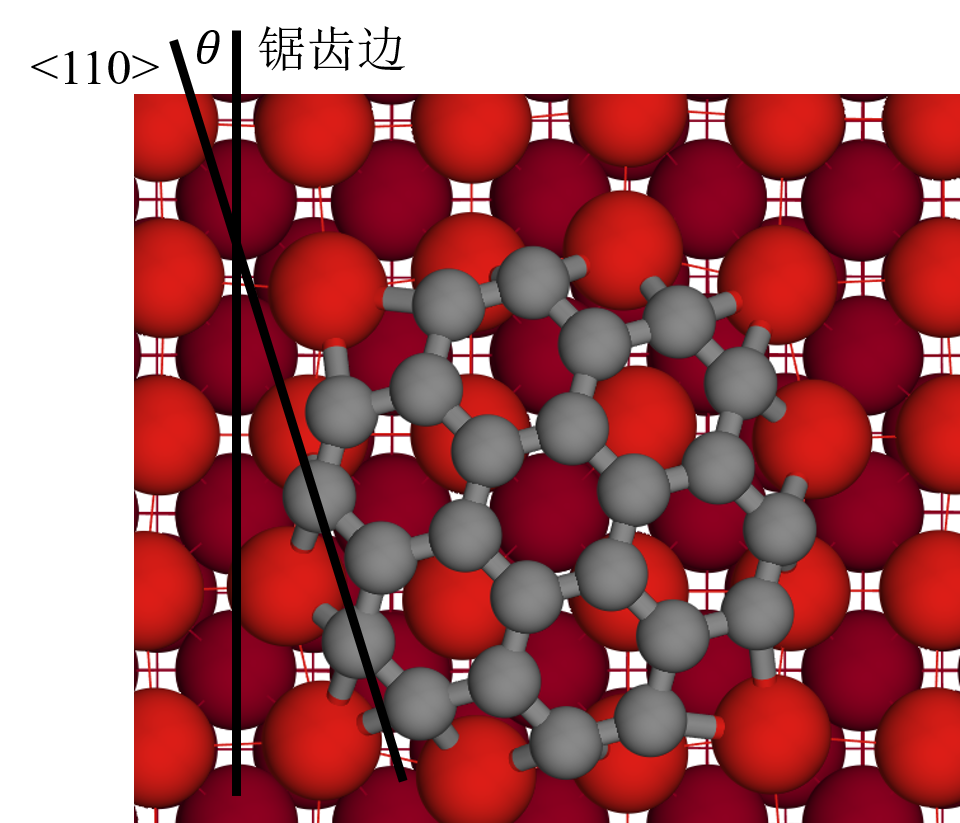
\includegraphics[width=0.4\textwidth]{pic/GO_relativeAngle.png}
    }
    \caption{计算流程图以及$\CCluster{24}$团簇生长角度标识示意图。(a)计算流程图;(b)$\CCluster{24}$团簇在铜衬底上的生长相对角度标识,其中,碳原子为灰色,铜原子为红色,不同层的铜原子以不同亮度进行区分。}
    \label{fig:GO_calculateFlow_relativeAngle}
\end{figure}

\subsection{石墨烯在平坦铜表面的生长晶向}
我们首先研究石墨烯$\CCluster{24}$团簇在平坦的铜衬底表面的优先生长晶向。如图\ref{fig:GO_001_15_structure}所示,在铜(001)晶面,我们的计算发现当$\CCluster{24}$团簇中央的空洞位于铜衬底表面的面心立方(fcc)位(图\ref{fig:GO_001_15_structure_top}),同时生长角度位$\SI{15}{\degree}$时,形成能最低。同时,计算获得的$\CCluster{24}$团簇在铜(001)表面的次优生长方向为$\SI{0}{\degree}$,与先前的文献符合\citing{RN692-2015}。从原子结构上看,石墨烯$\CCluster{24}$团簇边缘的碳原子与衬底表面的铜原子具有较强的相互作用。边缘碳原子与衬底表面铜原子的成键使得$\CCluster{24}$团簇的中央拱起,同时也使得$\CCluster{24}$团簇向更多边缘成键的角度旋转,由此在铜(001)表面形成了$\SI{15}{\degree}$的优先生长方向。

\begin{figure}[htb]
    \subfloat[]{
        \label{fig:GO_001_15_structure_side}
        \begin{overpic}[width=0.4\textwidth]{pic/GO_C24_flat_001_15deg_structure_side.png}
            \put(85,75){$(0 0 1)$}
        \end{overpic}
    }
    \subfloat[]{
        \label{fig:GO_001_15_structure_top}
        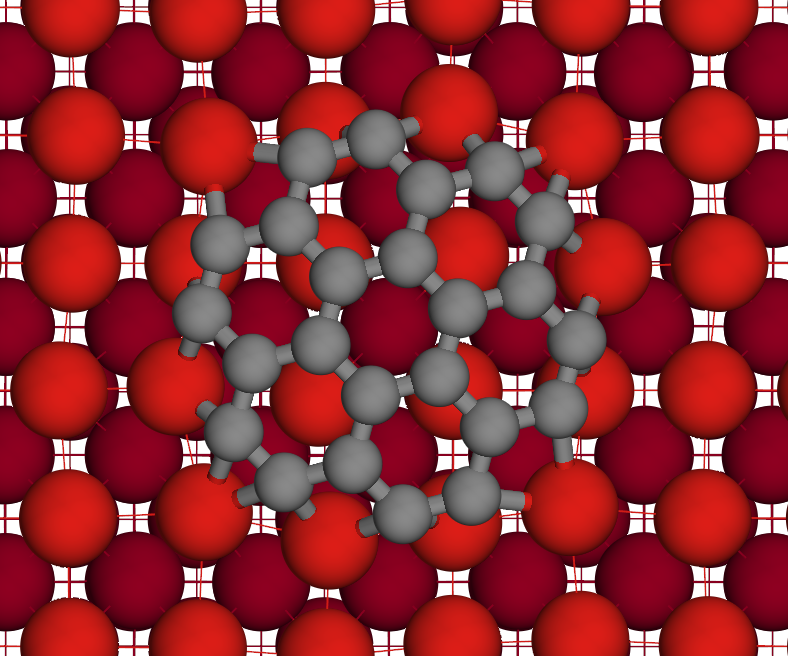
\includegraphics[width=0.4\textwidth]{pic/GO_C24_flat_001_15deg_structure_top.png}
    }

    \caption{铜(001)晶面石墨烯$\CCluster{24}$团簇的最优生长晶向(\SI{15}{\degree})及原子构型。(a)原子构型侧视图;(b)原子构型俯视图。图中,碳原子为灰色,铜原子为红色,不同层的铜原子以不同亮度进行区分。}
    \label{fig:GO_001_15_structure}
\end{figure}

接着,我们进一步计算了$\CCluster{24}$团簇在铜(001)表面各个角度的相对形成能,结果如图\ref{fig:GO_001_energy}所示。可以看到,$\CCluster{24}$团簇在平坦的铜(001)表面具有两个不重合的能量最小值,分别位于$\SI{+15}{\degree}$和$\SI{-15}{\degree}$。$\CCluster{24}$团簇在$\SI{0}{\degree}$和$\SI{30}{\degree}$的生长方向处于能量最高值。从能量最高的生长角度到能量最低的生长角度,$\CCluster{24}$团簇在中间态的相对能量逐渐下降。由于$\CCluster{24}$团簇在旋转至最低能态的过程中均为放热反应,因此绝大部分在成核阶段未处于最优生长方向的石墨烯晶畴会在热力学的作用下逐渐向$\SI{\pm 15}{\degree}$ 的生长晶向靠拢。在铜(001)表面,$\SI{\pm 15}{\degree}$ 的石墨烯$\CCluster{24}$团簇互为镜面对称,具有相同的形成能。因此在成核生长的过程中,约有一半的石墨烯畴会采取$\SI{-15}{\degree}$的晶向生长,而另一半则会生长为$\SI{+15}{\degree}$的石墨烯畴。从原子结构的角度来看,互为镜像的$\SI{\pm 15}{\degree}$ 石墨烯畴在几何上并不重叠,由此导致了许多实验中观察到的石墨烯晶畴的非定向生长\citing{RN1062-2012}。

\begin{figure}[htb]
    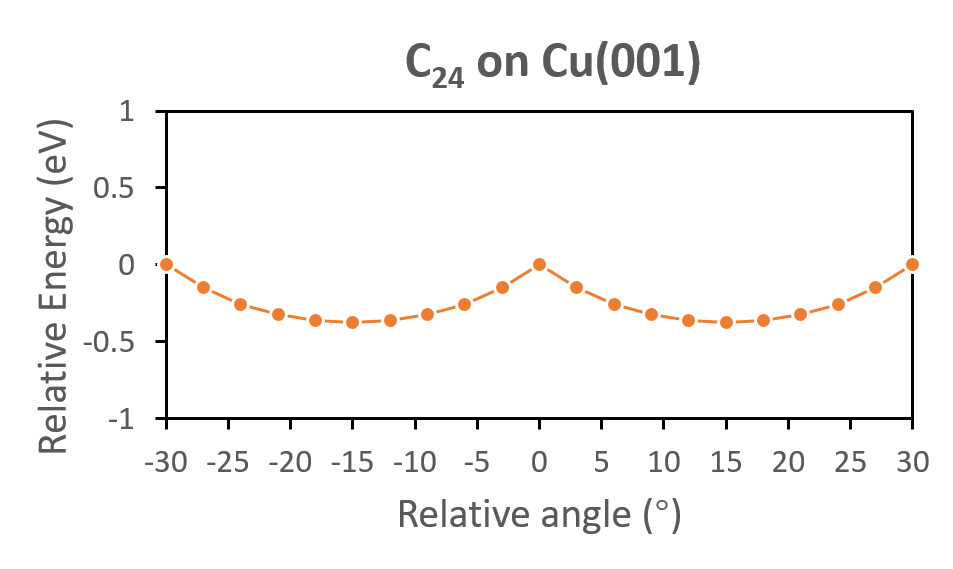
\includegraphics[width=0.8\textwidth]{pic/GO_C24_flat_001_energy.png}

    \caption{铜(001)晶面上不同生长角度的石墨烯$\CCluster{24}$团簇的相对形成能分布。各生长角度相对形成能的参考构型为生长角度$\SI{0}{\degree}$的构型。
    }

    \label{fig:GO_001_energy}
\end{figure}

而对于铜(111)面,$\CCluster{24}$团簇在其上生长的情况与在铜(001)面类似。我们同样计算了$\CCluster{24}$团簇在平坦的铜(111)表面的最优生长位点和最优生长方向。如图\ref{fig:GO_111_structure}所示,不同于在铜(001)表面,$\CCluster{24}$团簇在平坦的铜(111)表面面上的最优生长位点为团簇中央空位垂直于铜(111)表面原子的顶端(图\ref{fig:GO_111_structure_top})。经过优化后的$\CCluster{24}$团簇的最优生长角度为$\SI{\pm 18}{\degree}$。$\CCluster{24}$团簇边缘的碳原子同样也和铜(111)衬底表面的铜原子形成了较强的键合,使$\CCluster{24}$团簇呈现处拱起的几何形貌。$\CCluster{24}$团簇在铜(111)表面和铜(001)表面优先生长位点和方向的不同可能是来源于不同晶面指数表面对称性的变化。对于单层的铜(001)表面,其空间对称群为$P4/mmm$,为四方对称。对于单层的铜(111)表面,其空间对称群为$P6/mmm$,为六方对称。

\begin{figure}[htb]
    \subfloat[]{
        \label{fig:GO_111_structure_side}
        \begin{overpic}[width=0.4\textwidth]{pic/GO_C24_flat_111_18deg_structure_side.png}
            \put(80,75){$(1 1 1)$}
        \end{overpic}
    }
    \subfloat[]{
        \label{fig:GO_111_structure_top}
        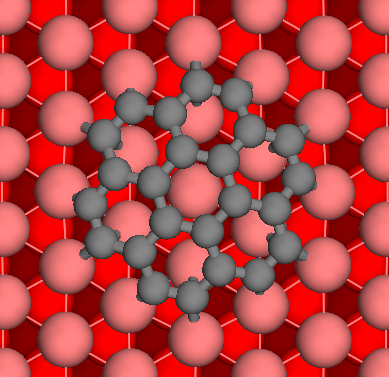
\includegraphics[width=0.4\textwidth]{pic/GO_C24_flat_111_18deg_structure_top.png}
    }

    \caption{铜(111)晶面石墨烯$\CCluster{24}$团簇的最优生长晶向($\SI{18}{\degree}$)及原子构型。(a)原子构型侧视图;(b)原子构型俯视图。图中,碳原子为灰色,铜原子为红色,不同层的铜原子以不同亮度进行区分。
    }

    \label{fig:GO_111_structure}
\end{figure}

通过插值法,我们对平坦铜(111)表面的石墨烯$\CCluster{24}$团簇在最优生长角度之间的中间态也进行了形成能计算(图\ref{fig:GO_111_energy})。$\CCluster{24}$团簇在铜(111)上的次优生长方向为$\SI{\pm 30}{\degree}$。由于衬底对称性的变化,在铜(111)表面,$\SI{0}{\degree}$ 方向生长的$\CCluster{24}$团簇与$\SI{\pm 30}{\degree}$方向生长的$\CCluster{24}$团簇并不等价。具体而言,遵循$\SI{0}{\degree}$ 方向生长的$\CCluster{24}$团簇的锯齿(zigzag)边与铜(111)衬底的<110>方向平行,扶手椅(armchair)边与$<\bar{1}\bar{1}2>$方向平行。而遵循$\SI{\pm 30}{\degree}$方向生长的$\CCluster{24}$团簇则相反,扶手椅(armchair)边与铜(111)衬底的<110>方向平行,锯齿(zigzag)边与$<\bar{1}\bar{1}2>$方向平行。铜$<\bar{1}\bar{1}2>$晶向的原子间距为$\SI{4.23}{\angstrom}$,高于铜<110>晶向中$\SI{2.56}{\angstrom}$的铜原子间距。从计算结果上看,$\SI{\pm 30}{\degree}$方向生长的$\CCluster{24}$团簇的形成能比$\SI{0}{\degree}$ 方向生长的$\CCluster{24}$团簇低大约$\SI{0.9}{\electronvolt}$。与在平坦的铜(001)晶面上类似,$\CCluster{24}$团簇从任意生长角度到能量最低的$\SI{\pm 18 }{\degree}$的中间态的能量逐渐下降。$\CCluster{24}$团簇在转向最优生长角度的过程均为放热反应,因此绝大部分在成核阶段未处于最优生长方向的石墨烯晶畴会在热力学的作用下逐渐向$\SI{\pm 18}{\degree}$ 的生长晶向靠拢。从原子结构的角度来看,互为镜像的$\SI{\pm 18}{\degree}$ 石墨烯畴在几何上并不重叠。在生长过程中的不同晶畴进行融合时仍会产生晶界。

\begin{figure}[htb]
    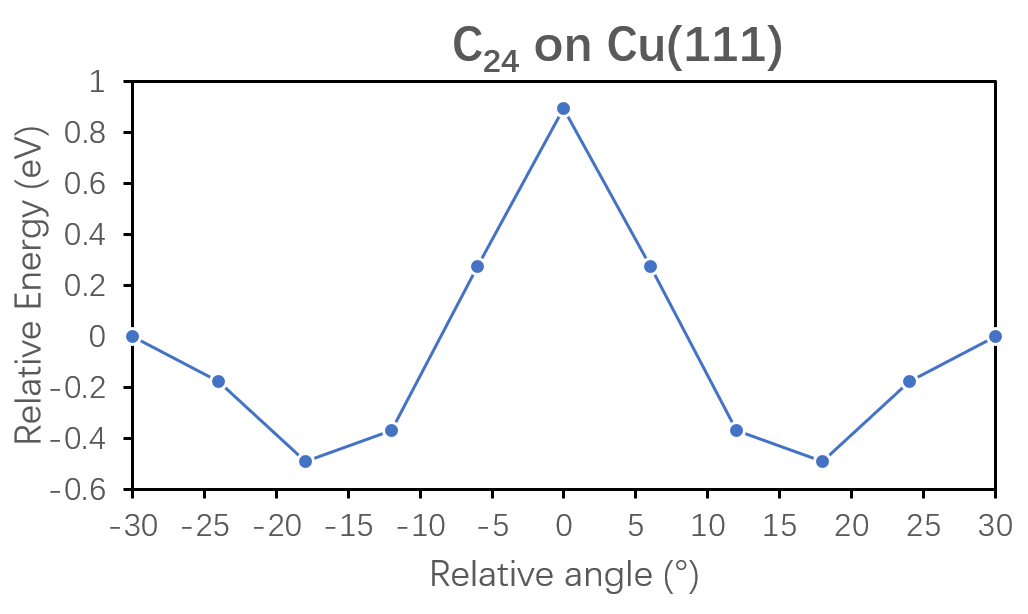
\includegraphics[width=0.8\textwidth]{pic/GO_C24_flat_111_energy.png}
    \caption{铜(111)晶面上不同生长角度的石墨烯$\CCluster{24}$团簇的相对形成能分布。各生长角度相对形成能的参考构型为生长角度$\SI{\pm 30}{\degree}$的构型。
    }
    \label{fig:GO_111_energy}
\end{figure}

\subsection{石墨烯在铜表面台阶处的生长晶向}
在本章的研究中,我们主要关注石墨烯$\CCluster{24}$团簇在晶面指数为$\rm{(11n)(n \geqslant 1)}$的铜衬底的优先生长晶向。晶面指数为$\rm{(11n)(n \geqslant 1)}$的铜表面结构可以看成由不同密度的铜(001)台面或者铜(111)台面组合而成。因此,我们可以将晶面指数为$\rm{(11n)(n \geqslant 1)}$的铜衬底分为两类\chinesecolon 一类可以看作以铜(001)台面组合而成,台阶的方向为铜<110>晶向,这类同衬底的晶面指数为$\rm{(11n)(n \geqslant 3)}$。另一类可以看作以铜(111)台面组合,台阶方向同样为铜<110>晶向,这类铜衬底的晶面指数为$\rm{(11n)(1 \leqslant n \leqslant 3)}$。而作为二者之间的铜(113)晶面,是两原子宽的铜(001)晶面加上两原宽的铜(111)晶面相对搭接而成。因此,在铜(113)表面的台阶,既可以看成是(001)台面,也可以看成是(111)台面。
%//TODO 11n 图,包括解剖

上一小节的计算显示,对于石墨烯$\CCluster{24}$团簇,其边缘碳原子与衬底表面铜原子的相互作用产生了$\CCluster{24}$团簇的优先生长角度。进一步的计算表明,$\CCluster{24}$团簇边缘碳原子在铜衬底表面的台阶处有相比于平坦衬底更强烈的相互作用(\ref{tab:GO_flat_vs_step})。具体而言,如果铜(001)衬底表面有一个晶向为<110>的台阶,$\CCluster{24}$团簇在台阶边缘的形成能为$E_{\rm f}^{\rm step}=\SI{-9.02}{\electronvolt}$,大大高于在平坦铜(001)衬底表面的形成能$E_{\rm f}^{\rm flat}=\SI{-6.24}{\electronvolt}$。因此,我们可以判断,石墨烯更倾向于在铜衬底的台阶处成核。

\begin{table}
    \centering
    \caption{石墨烯$\CCluster{24}$团簇在平坦铜(001)衬底以及<100>台阶边缘的形成能}
    \begin{tabular}{cc}
        \toprule
        衬底类型                     & 形成能(\si{\electronvolt}) \\
        \midrule
        平坦铜(001)衬底            & $-6.24$                      \\
        铜(001)衬底的<110>台阶边缘 & $-9.02$                      \\
        \bottomrule
    \end{tabular}
    \label{tab:GO_flat_vs_step}
\end{table}

对于以铜(001)为台面的铜$\rm{(11n)(n \geqslant 3)}$衬底。由于石墨烯团簇与铜衬底的相互作用主要集中在团簇边缘的未饱和碳原子。并且台阶作为台面的边缘会极大的影响石墨烯团簇与铜衬底的形成能。为了不失一般性,我们以$\CCluster{24}$团簇的直径作为参考,我们建立了三个代表性的铜衬底模型。
这三个模型分别对应于台面长度小于$\CCluster{24}$团簇直径的铜(115)晶面;台面长度大致等于$\CCluster{24}$团簇直径的铜(117)晶面;以及台面长度远大于小于$\CCluster{24}$团簇直径的$\rm (11X)(X \gg 7 )$晶面。

对于台面长度远大于小于$\CCluster{24}$团簇直径的$\rm (11X)(X \gg 7 )$晶面(图\ref{fig:GO_C24_11X}),计算结果显示当$\CCluster{24}$团簇在台阶处成核生长时$\CCluster{24}$团簇的最优成核位置位于台阶的下方(图\ref{fig:GO_11X_structure_side}和图\ref{fig:GO_11X_structure_top}),$\CCluster{24}$团簇的中央空洞位于铜(001)台面的六方密堆(hcp)位。此时一半的$\CCluster{24}$团簇边缘与铜<110>台阶成键,另一半与铜(001)台面成键。相对于在平坦的铜(001)表面,$\CCluster{24}$团簇在铜(11X)表面的两个不重叠的最优生长角度,由于台阶的作用产生了劈裂和偏移,出现了最优生长角度和次优生长角度。

%figure 11X
\begin{figure}[!htb]
    \centering
    \subfloat[]{
        \label{fig:GO_11X_structure_side}
        \begin{overpic}[width=0.4\textwidth,trim={40 0 40 0},clip]{pic/GO_11X_structure_side.png}
            \put(85,60){$\rm (1 1 X)$}
        \end{overpic}
    }
    \subfloat[]{
        \label{fig:GO_11X_structure_top}
        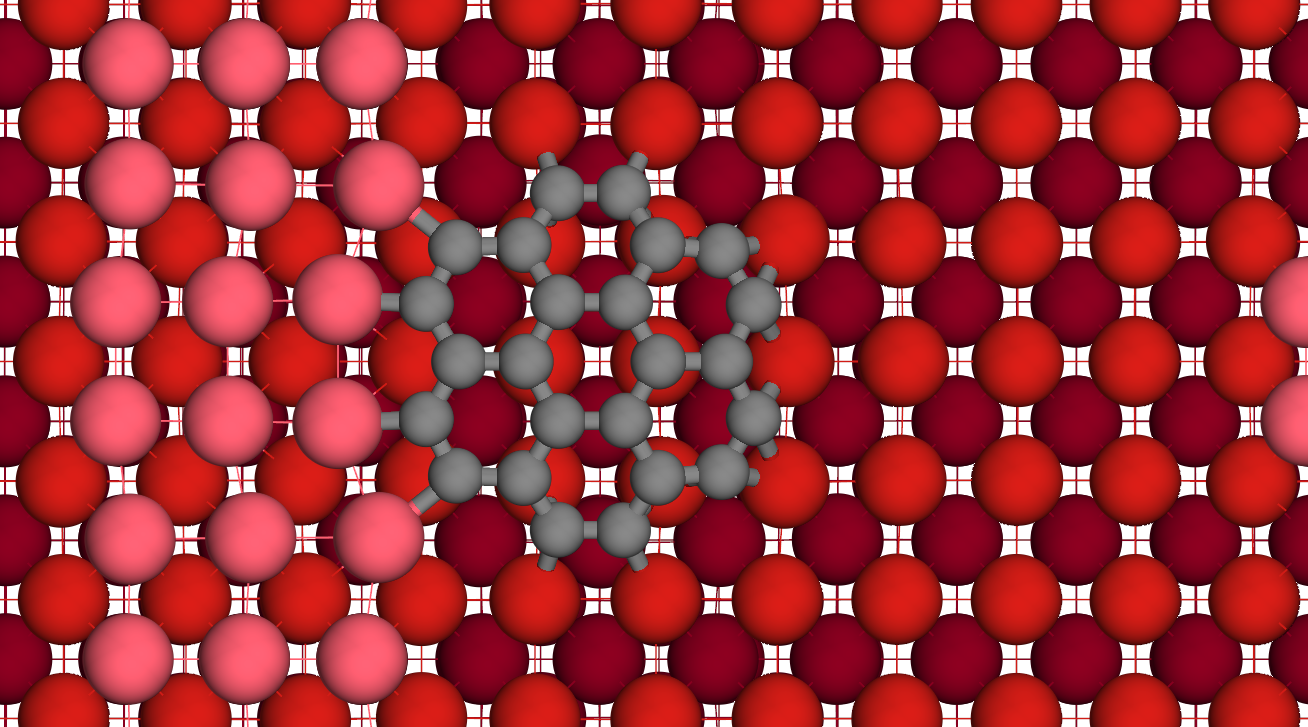
\includegraphics[width=0.4\textwidth,trim={60 20 150 20},clip]{pic/GO_11X_structure_top.png}
    }\\[-0.5ex]
    \subfloat[]{
        \label{fig:GO_11X_structure_energy}
        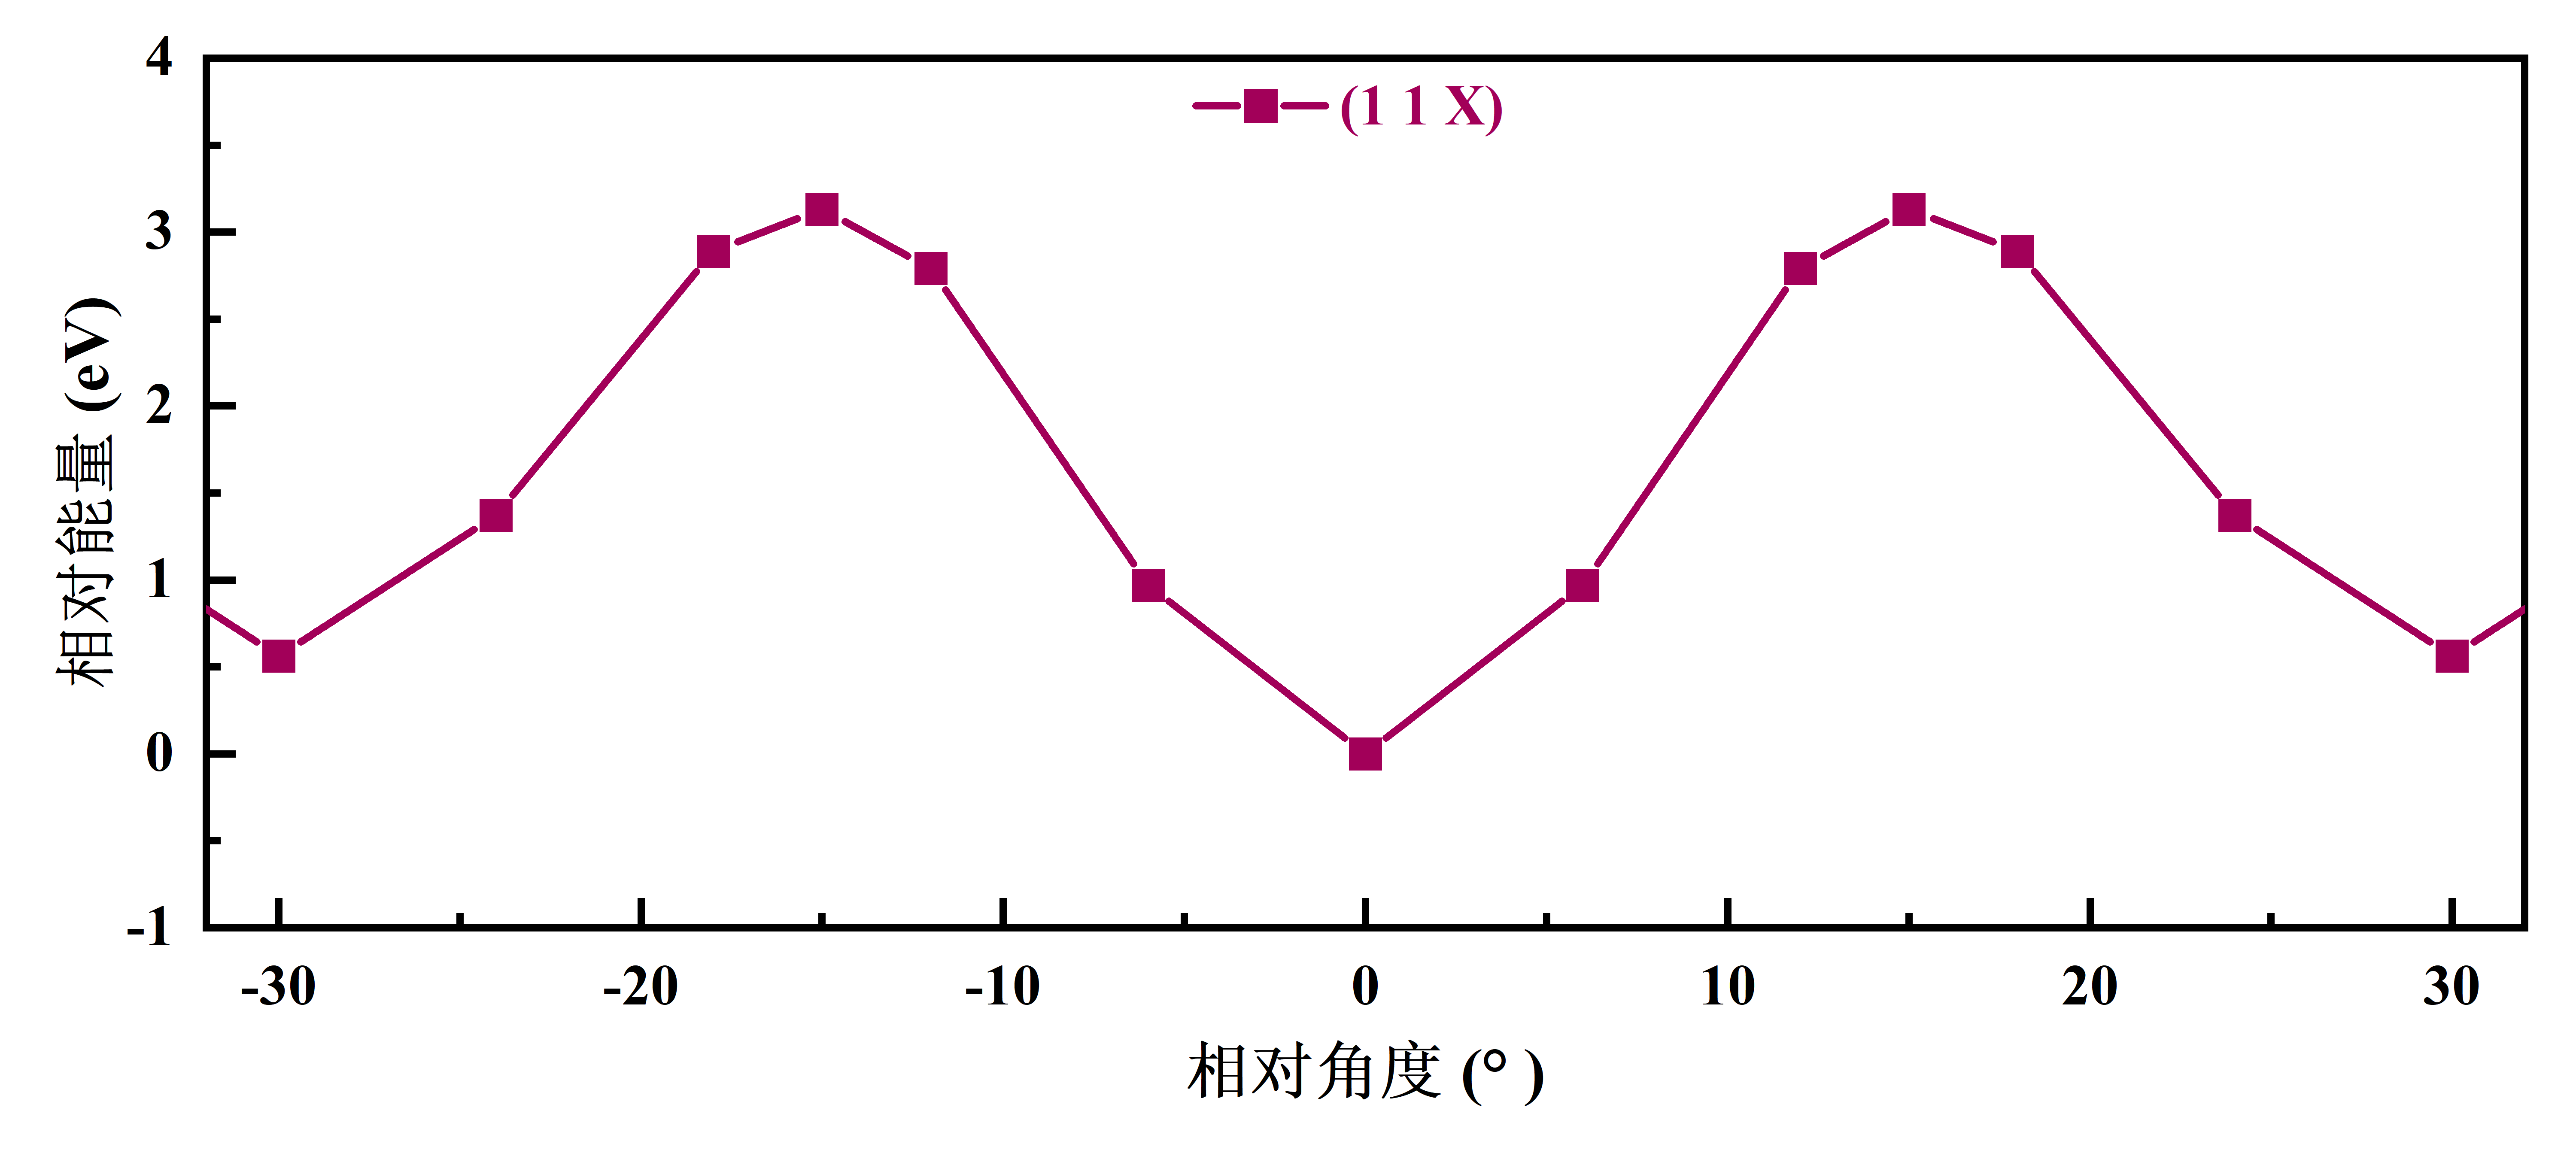
\includegraphics[width=0.8\textwidth]{pic/GO_C24_11X_energy.png}
    }
    \caption{铜(11X)晶面上石墨烯$\CCluster{24}$团簇的最优生长晶向(\SI{0}{\degree})、原子构型以及各生长角度能量分布图。(a)原子构型侧视图;(b)原子构型俯视图;(c)各生长角度能量分布。图中,碳原子为灰色,铜原子为红色,不同层的铜原子以不同亮度进行区分。}
    \label{fig:GO_C24_11X}
\end{figure}

从图\ref{fig:GO_11X_structure_energy}中可以看到,$\CCluster{24}$团簇在铜(11X)表面的台阶处的最优生长角度为$\SI{0}{\degree}$,次优生长角度为$\SI{\pm 30 }{\degree}$。最优和次优生长角度之间的能量差为$\SI{0.56 }{\electronvolt}$。$\SI{\pm 30 }{\degree}$和$\SI{0}{\degree}$的生长角度之间,有约为$\SI{2.56}{\electronvolt}$的旋转势垒。单一的最优生长角度使得$\CCluster{24}$团簇在铜(11X)衬底的台阶处展现出定向生长的趋势。较高的旋转势垒使得$\CCluster{24}$团簇在成核生长的过程中需要需要较高的温度才能从次优的$\SI{\pm 30 }{\degree}$生长角度旋转至最优的$\SI{0 }{\degree}$。同时,由于铜(11X)衬底的(001)台面具有高于$\CCluster{24}$团簇直径的宽度,因此石墨烯晶畴很可能在远离<001>台阶的位置成核生长。在远离<001>台阶的位置成核生长的石墨烯晶畴类似于在平坦铜(001)衬底的表面生长。此时生长的石墨烯晶畴则缺乏热力学上的定向趋势。因此在铜(11X)乃至于铜(001)表面很难实现石墨烯晶畴的定向生长。

$\CCluster{24}$团簇在铜(117)以及(115)晶面的台阶处的生长情况与铜(11X)表面相似(图\ref{fig:GO_C24_117_115})。在铜(117)晶面上,由于(001)台面的宽度与$\CCluster{24}$团簇的直径相近,$\CCluster{24}$团簇的一边与第一层台阶下边缘成键,另一层与第二层台阶的上边缘成键(图\ref{fig:GO_117_structure_side}和图\ref{fig:GO_117_structure_top})。$\CCluster{24}$团簇在铜(117)表面的最优生长位置同样也为铜(001)台面的六方密堆(hcp)位。而对于铜(115)晶面台阶处的$\CCluster{24}$团簇生长,由于铜(115)晶面上的铜(001)台面宽度仅有2原子宽,短于$\CCluster{24}$团簇的直径,所以$\CCluster{24}$团簇无法与第一层台阶的下边缘成键(图\ref{fig:GO_115_structure_side}和图\ref{fig:GO_115_structure_top})。导致在铜(115)晶面上,$\CCluster{24}$团簇的一边与第二层的台面成键,另一边与第三层台阶的上边缘成键。与第二层台阶具有较强相互作用的则是位于$\CCluster{24}$团簇中部的边缘原子。同时,由于$\CCluster{24}$团簇在(115)晶面上的生长需要横跨两层台阶,其最优生长位点相对于(11X)以及(115)晶面也有所变化。正对$\CCluster{24}$团簇中央空位的衬底位点由在(001)台面上的六方密堆(hcp)位移动至面心立方(fcc)位。

%figure 117 115
\begin{figure}[!htb]
    \subfloat[]{
        \label{fig:GO_117_structure_side}
        \begin{overpic}[width=0.4\textwidth,trim={60 40 40 0},clip]{pic/GO_117_structure_side.png}
            \put(85,53){$(1 1 7)$}
        \end{overpic}
    }
    \subfloat[]{
        \label{fig:GO_117_structure_top}
        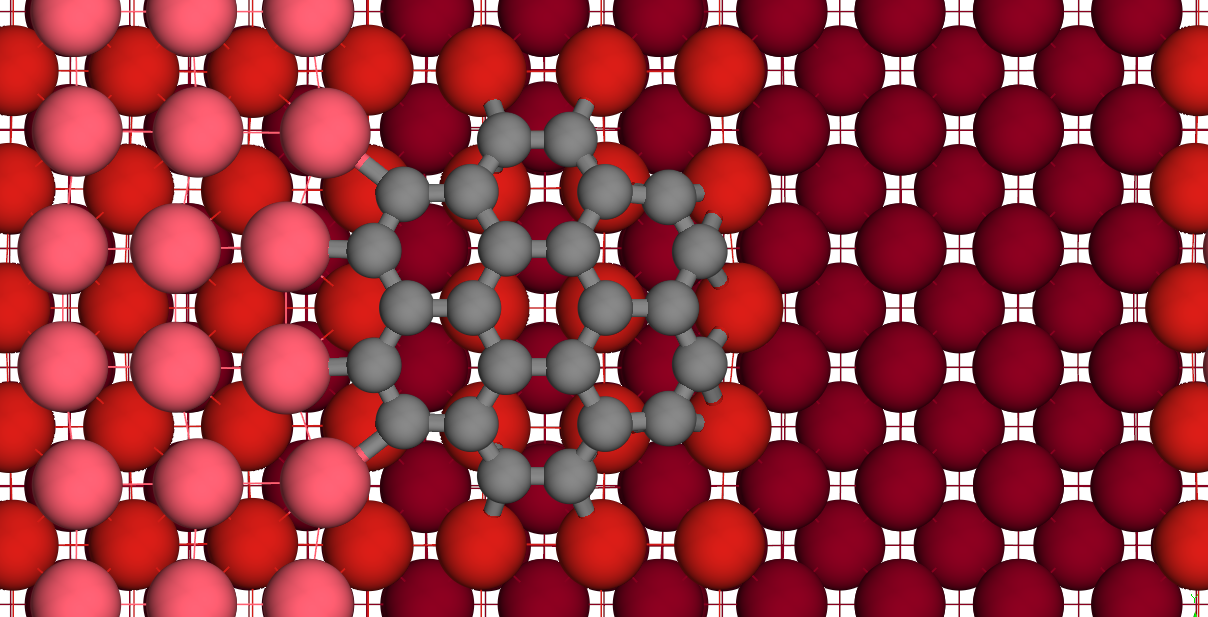
\includegraphics[width=0.4\textwidth,trim={40 0 60 0},clip]{pic/GO_117_structure_top.png}
    }\\[-1ex]
    \subfloat[]{
        \label{fig:GO_115_structure_side}
        \begin{overpic}[width=0.4\textwidth,trim={60 80 40 10},clip]{pic/GO_115_structure_side.png}
            \put(85,53){$(1 1 5)$}
        \end{overpic}
    }
    \subfloat[]{
        \label{fig:GO_115_structure_top}
        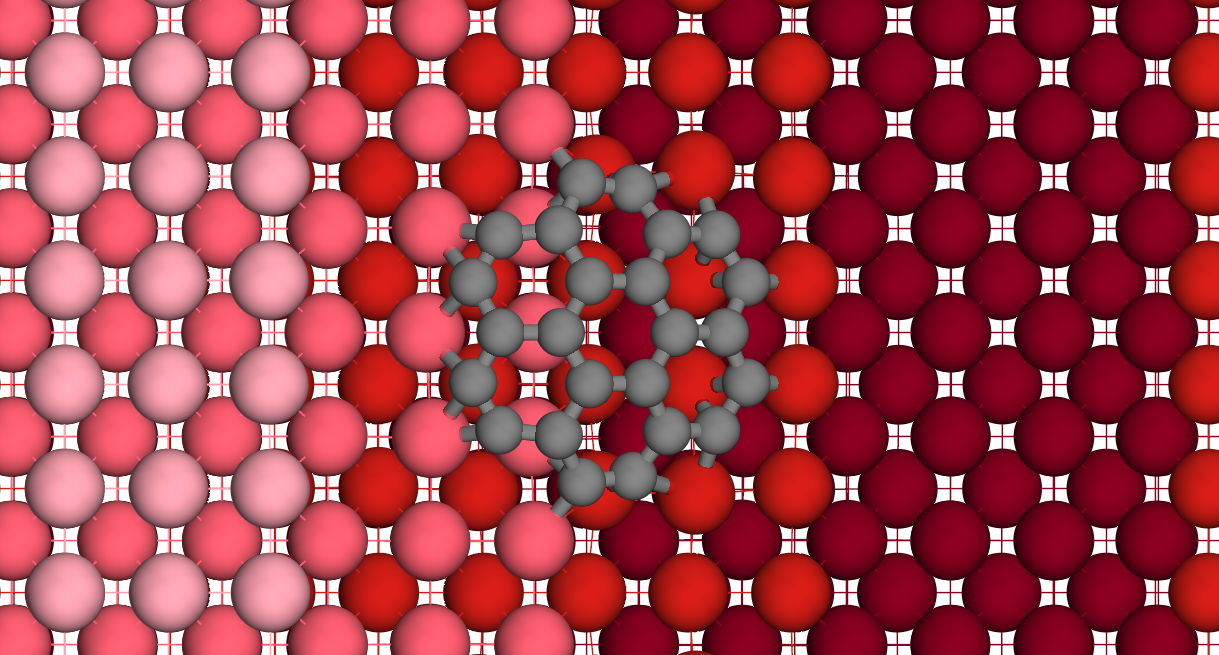
\includegraphics[width=0.4\textwidth,trim={60 20 120 40},clip]{pic/GO_115_structure_top.png}
    }\\[-0.5ex]
    \subfloat[]{
        \label{fig:GO_C24_117_115_energy}
        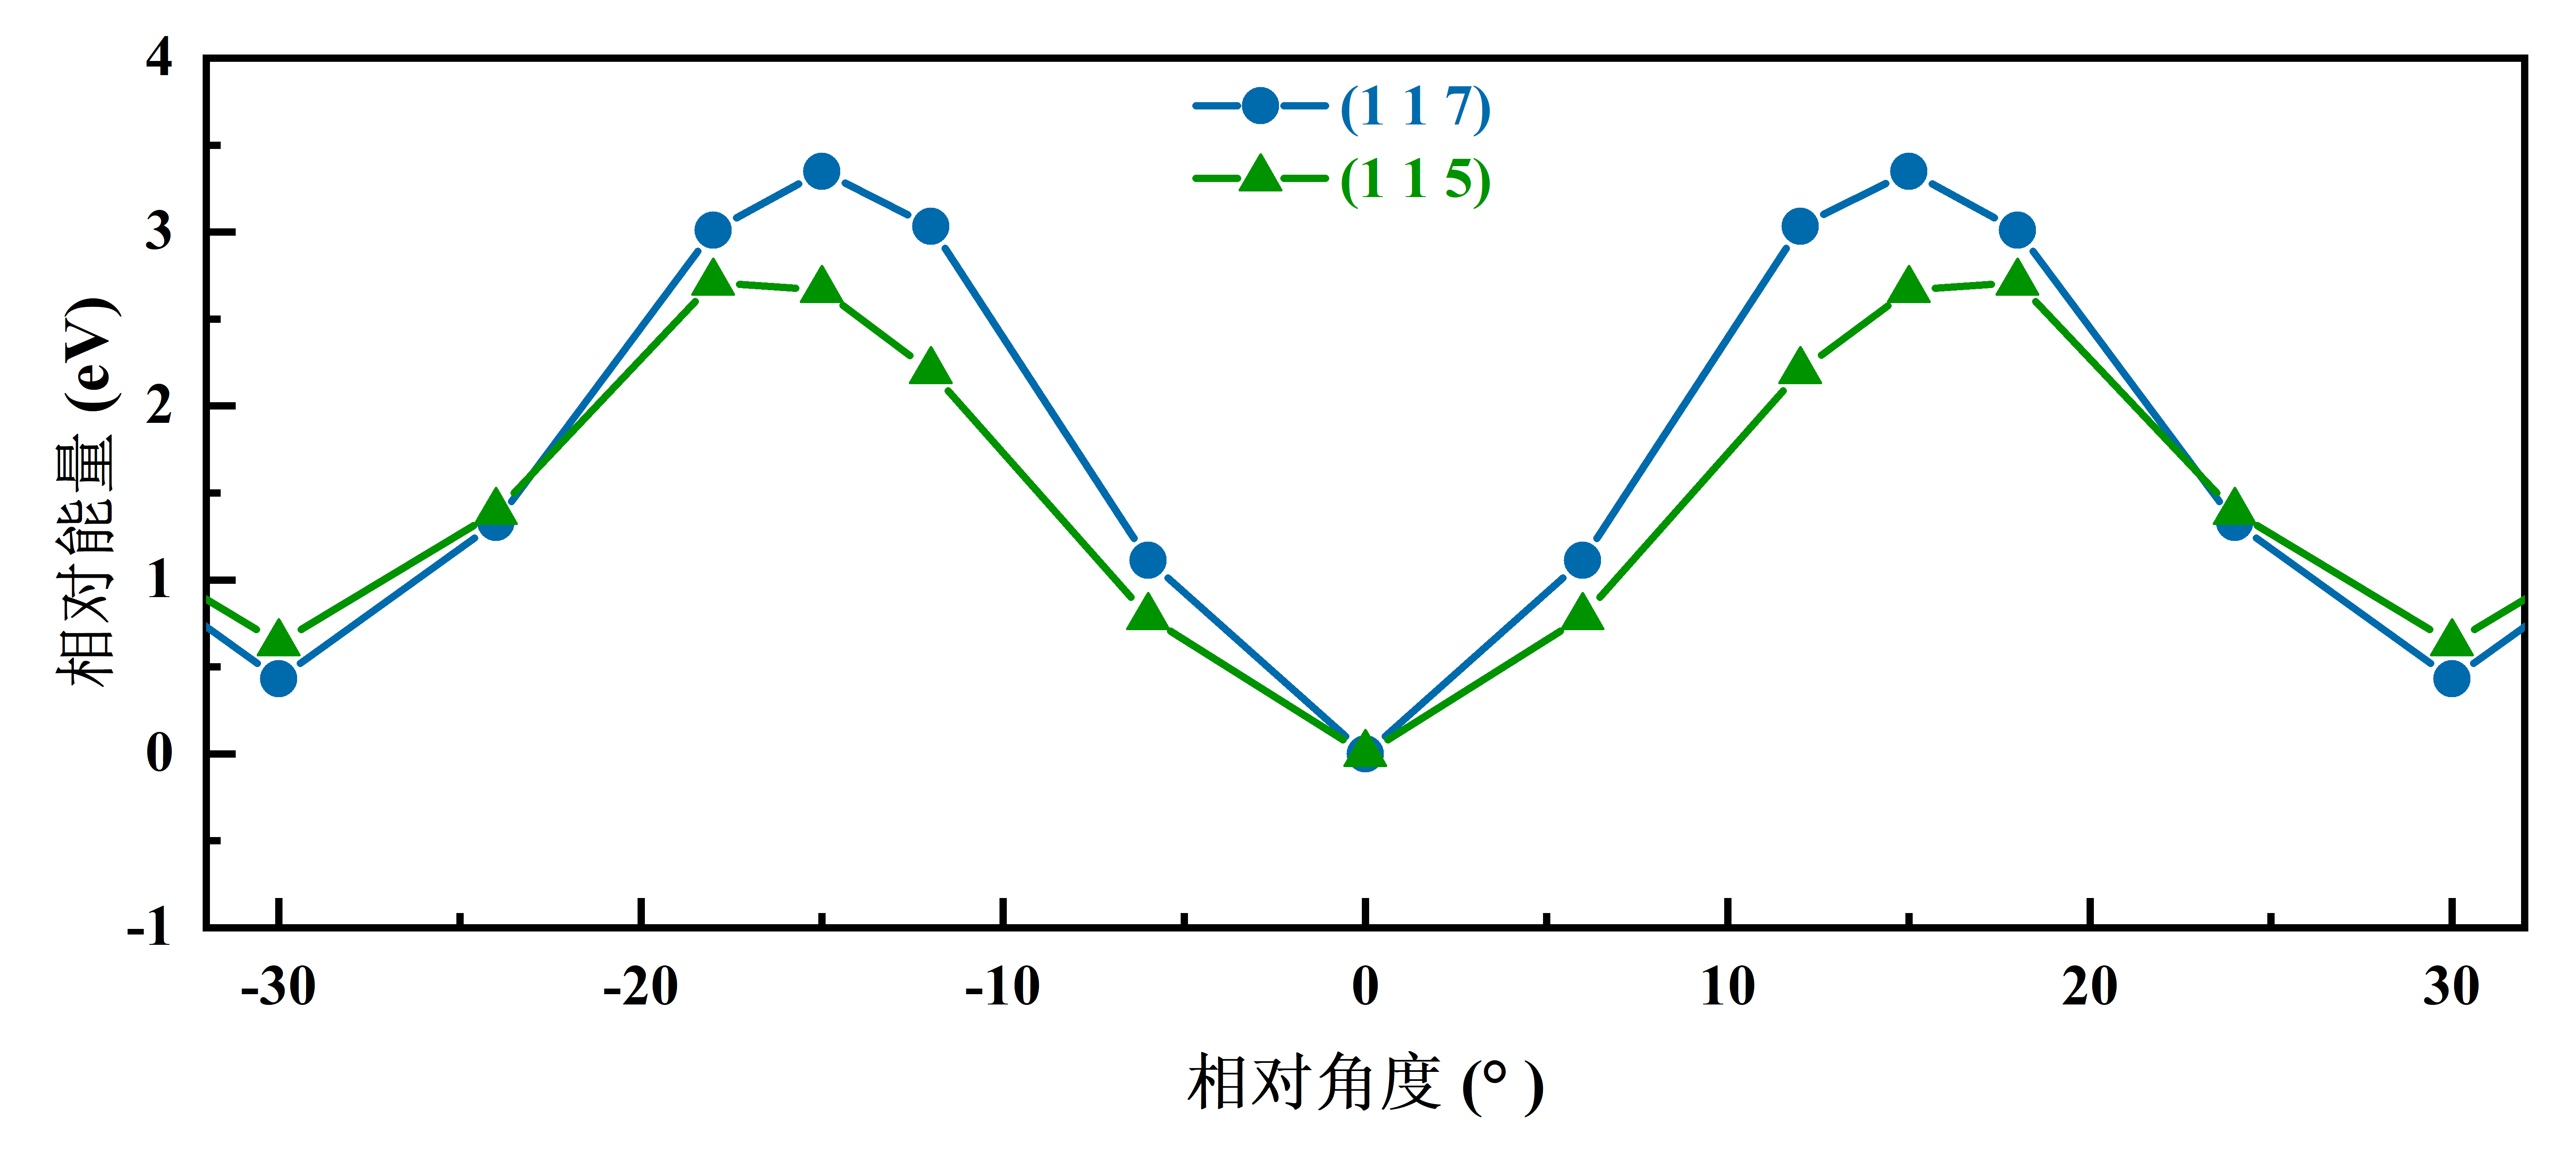
\includegraphics[width=0.8\textwidth]{pic/GO_C24_117_115_energy.png}
    }
    \caption{铜(117)与(115)晶面上石墨烯$\CCluster{24}$团簇的最优生长晶向(\SI{0}{\degree})、原子构型以及各生长角度能量分布图。(a)(117)晶面原子构型侧视图;(b)(117)晶面俯视图;(c)(115)晶面最优生长角度原子构型侧视图;(d)(115)晶面俯视图;(e)(117)与(115)晶面上$\CCluster{24}$团簇各生长角度能量分布。图中,碳原子为灰色,铜原子为红色,不同层的铜原子以不同亮度进行区分。}
    \label{fig:GO_C24_117_115}
\end{figure}

从能量的角度上看(图\ref{fig:GO_C24_117_115_energy}),$\CCluster{24}$团簇在铜(117)以及(115)晶面的上的最优生长角度均为$\SI{0 }{\degree}$,次优生长角度位$\SI{\pm 30 }{\degree}$,与铜(11X)晶面台阶处一致。在铜(117)晶面上,$\CCluster{24}$团簇在次优生长角度和最优生长角度之间的能量差为$\SI{0.43}{\electronvolt}$。这个能量差低于$\CCluster{24}$团簇在铜(11X)晶面台阶边缘的$\SI{0.56}{\electronvolt}$次优-最优角能量差,导致在铜(117)晶面上$\CCluster{24}$团簇从次优生长角转向最优生长角的比例不及生长在(11X)晶面台阶处的$\CCluster{24}$团簇,使得铜(117)晶面上生长的石墨烯的定向性下降。同时,$\CCluster{24}$团簇从次优的$\SI{\pm 30 }{\degree}$生长角度转向最优的$\SI{0}{\degree}$需要克服的旋转势垒为$\SI{2.91 }{\electronvolt}$,同样高于$\CCluster{24}$团簇在铜(11X)晶面台阶处的旋转势垒。较高的旋转势垒会导致$\CCluster{24}$团簇从次优生长角向最优生长角的转变难度上升,需要更多的能量或者更长的时间才能反应至最稳态。由于石墨烯晶畴的成核生长与石墨烯晶畴向最优生长角的转变是同时进行的,石墨烯晶畴的进一步生长会引入更多的边缘原子与衬底键合,可能会导致旋转势垒提高到无法依靠热能逾越的地步。因此较高的旋转势垒也可能会导致石墨烯晶畴的定向性下降。对于铜(115)晶面,$\CCluster{24}$团簇在次优生长角度和最优生长角度之间的能量差为$\SI{0.64}{\electronvolt}$,高于铜(117)晶面以及铜(11X)晶面。同时对于$\CCluster{24}$团簇,在铜(115)晶面上成核生长时,在热力学的作用下从次优生长角度旋转至最优生长角度所需要跨越的旋转势垒为$\SI{2.07 }{\electronvolt}$,低于在铜(117)以及(11X)晶面的旋转势垒。

通过以上计算,我们可以发现,虽然台面的宽度有所差距,但是对于晶面指数为$\rm{(11n)(n \geqslant 3)}$铜衬底而言,衬底表面的台阶对石墨烯晶畴的生长方向均有限制作用。其中以(115)晶面铜衬底最能够使石墨烯晶畴依照以$\SI{0 }{\degree}$的生长角度进行定向成核生长。

%figure 112
\begin{figure}[htb]
    \subfloat[]{
        \label{fig:GO_112_structure_side}
        \begin{overpic}[width=0.4\textwidth,trim=30 20 20 0,clip]{pic/GO_112_structure_side.png}
            \put(85,53){$\rm (1 1 2)$}
        \end{overpic}
    }
    \subfloat[]{
        \label{fig:GO_112_structure_top}
        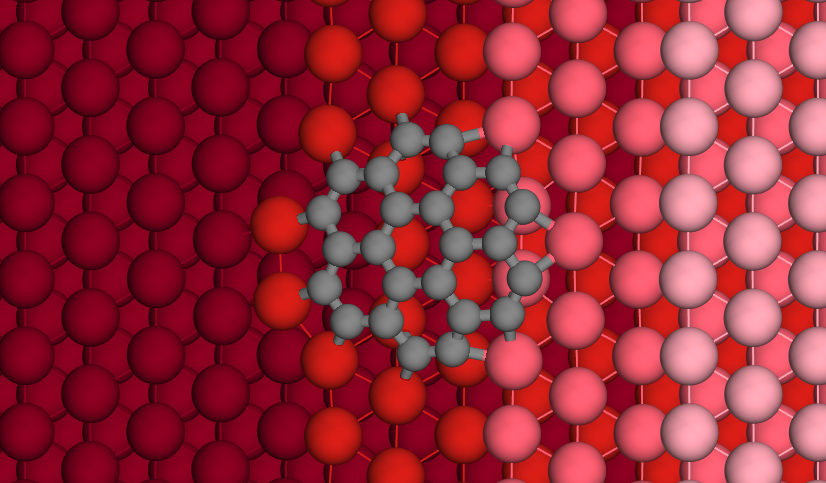
\includegraphics[width=0.4\textwidth,trim=80 40 50 40,clip]{pic/GO_112_structure_top.png}
    }\\[-0.5ex]
    \subfloat[]{
        \label{fig:GO_112_structure_energy}
        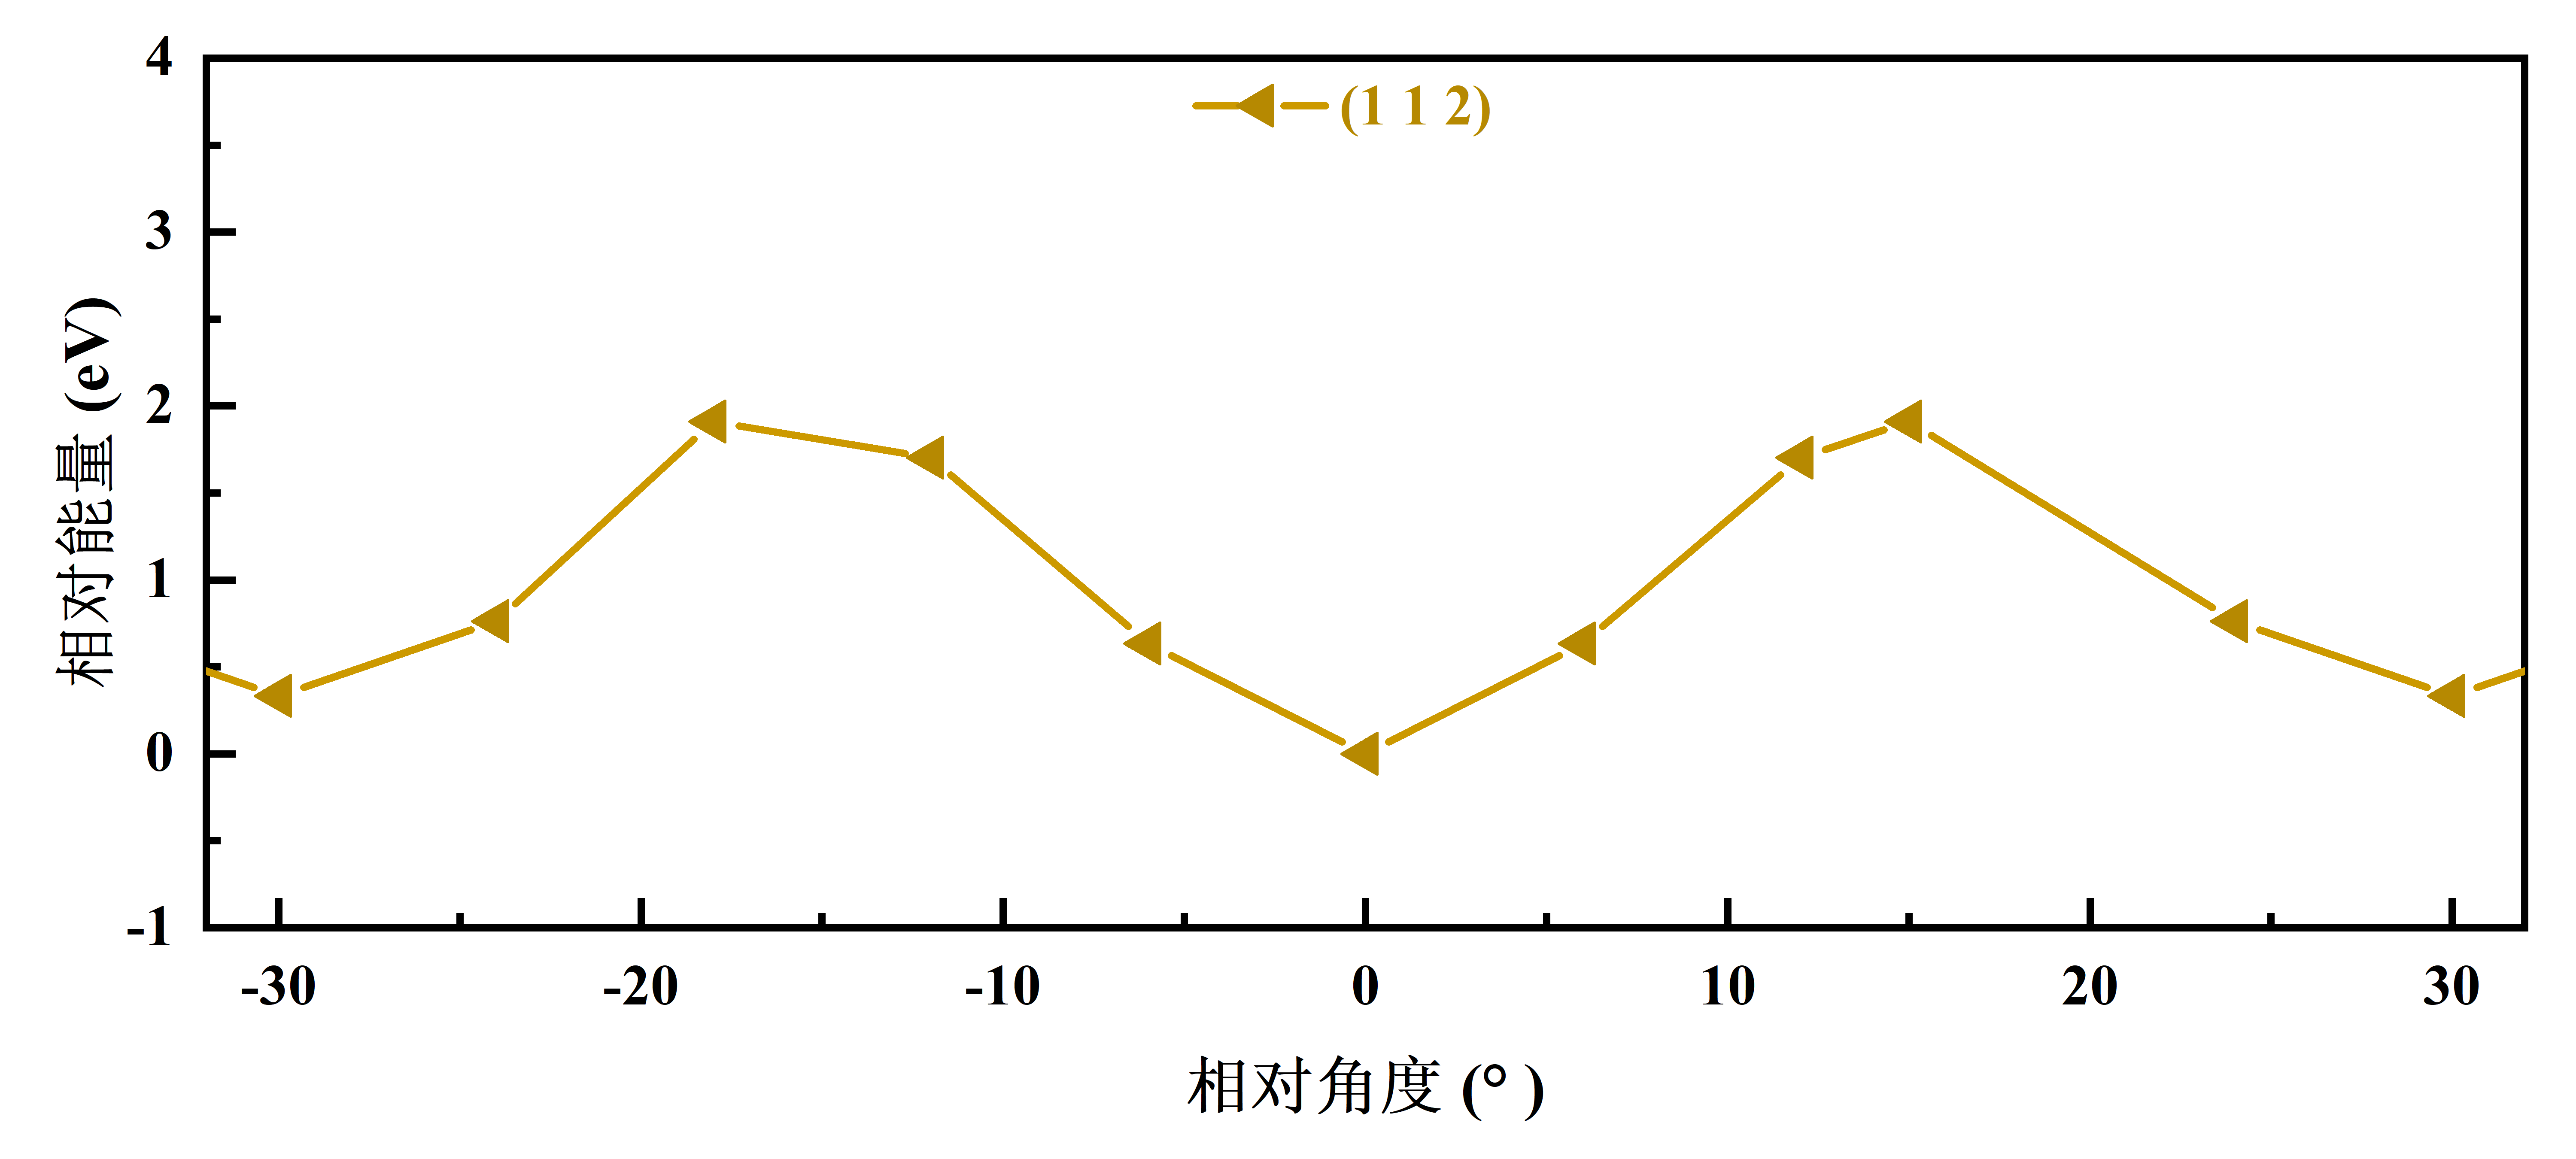
\includegraphics[width=0.8\textwidth]{pic/GO_C24_112_energy.png}
    }
    \caption{铜(112)晶面上石墨烯$\CCluster{24}$团簇的最优生长晶向(\SI{0}  {\degree})、原子构型以及各生长角度能量分布图。(a)最优生长角度原子构型侧视图;(b)最优生长角度原子构型俯视图;(c)各生长角度能量分布。图中,碳原子为灰色,铜原子为红色,不同层的铜原子以不同亮度进行区分。}
    \label{fig:GO_C24_112}
\end{figure}

对于以(111)为台面的铜(112)晶面,$\CCluster{24}$团簇在其台阶处的成核生长行为与在平坦的铜(111)衬底表面有较大的不同(图\ref{fig:GO_C24_112})。在铜(112)晶面,由于台面的宽度短于$\CCluster{24}$团簇的直径,$\CCluster{24}$团簇无法直接于第一层台阶的下边缘成键。优化后的最优构型显示$\CCluster{24}$团簇在铜(112)晶面上成核生长时倾向于跨越一层铜<110>台阶(图\ref{fig:GO_112_structure_side}和图\ref{fig:GO_112_structure_top})。$\CCluster{24}$团簇的一边与第一层的铜台面成键,另一边与第二层的铜台阶的上表面成键。在台阶的作用下,$\CCluster{24}$团簇在铜(112)台面上的最优生长方向为$\SI{0}{\degree}$。如图\ref{fig:GO_112_structure_energy}所示,台阶对于$\CCluster{24}$晶畴边缘碳原子较强的相互作用同样使得(111)台面上两个不重叠的最优生长角度($\SI{\pm 18 }{\degree}$)劈裂、偏移至$\SI{0}{\degree}$和$\SI{\pm 30 }{\degree}$。对于铜(112)晶面,$\CCluster{24}$团簇的最优生长角度为$\SI{0}{\degree}$,次优生长角度为$\SI{\pm 30 }{\degree}$。次优-最优生长角度之间的能量差为$\SI{0.33}{\electronvolt}$,低于先前计算的以铜(001)台面为基础的台阶模型。可以判断$\CCluster{24}$团簇在铜(112)衬底上的定向性弱于铜$\rm{(11n)(n \geqslant 3)}$衬底。旋转势垒方面,在铜(112)衬底上生长的石墨烯从次优的$\SI{\pm 30 }{\degree}$旋转至最优的$\SI{0}{\degree}$所需要克服的势垒为$\SI{1.57 }{\electronvolt}$,低于铜$\rm{(11n)(n \geqslant 3)}$衬底衬底。因此在铜(112)台面,石墨烯晶畴可以在更低的生长温度下从非定向生长演化为定向生长。

而对于铜(113)面,(001)台面和(111)台面的相互交错不仅使得铜(113)面具有在晶面指数为$\rm{(11n)(n \geqslant 1)}$这一系列的铜衬底中拥有最高的表面能\citing{RN1063-1993},同时也对石墨烯$\CCluster{24}$团簇的定向产生了极大的影响。从图\ref{GO_C24_113}中我们可以看到,在铜(113)面上,$\CCluster{24}$团簇的最优生长构型不仅横跨两个铜台面,同时团簇两边的边缘碳原子都与<110>台阶产生了强烈的相互作用。同时,$\CCluster{24}$团簇在铜(113)表面的最优生长角度也发生了变化,为几何相互不重叠的$\SI{\pm 27 }{\degree}$。因此,类似平坦的铜(001)表面以及铜(111)表面,石墨烯团簇在铜(113)表面无法实现能量上的定向生长。

%figure 113
\begin{figure}[htb]
    \subfloat[]{
        \label{fig:GO_113_structure_side}
        \begin{overpic}[width=0.4\textwidth, trim=20 20 20 30,clip]{pic/GO_113_structure_side.png}
            \put(85,45){$\rm (1 1 3)$}
        \end{overpic}
    }
    \subfloat[]{
        \label{fig:GO_113_structure_top}
        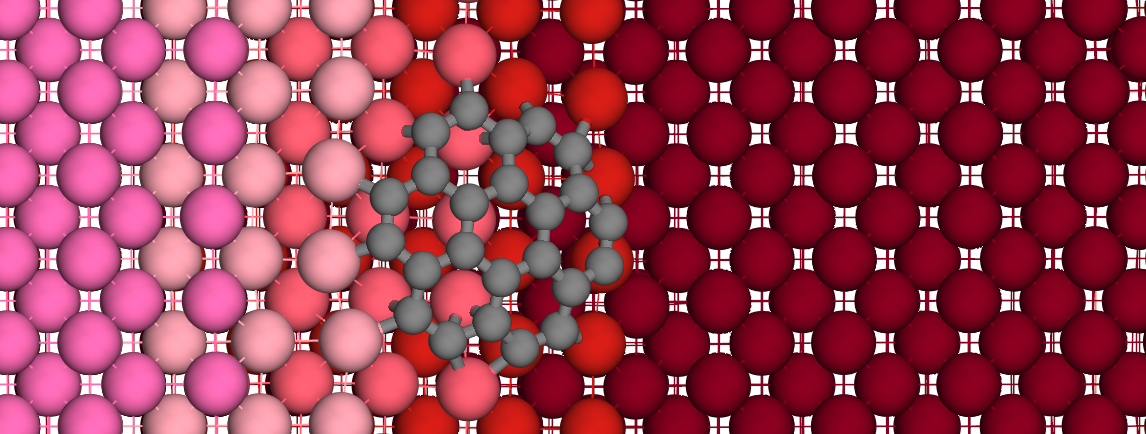
\includegraphics[width=0.4\textwidth,trim=80 0 150 0,clip]{pic/GO_113_structure_top.png}
    }\\[-0.5ex]
    \subfloat[]{
        \label{fig:GO_113_structure_energy}
        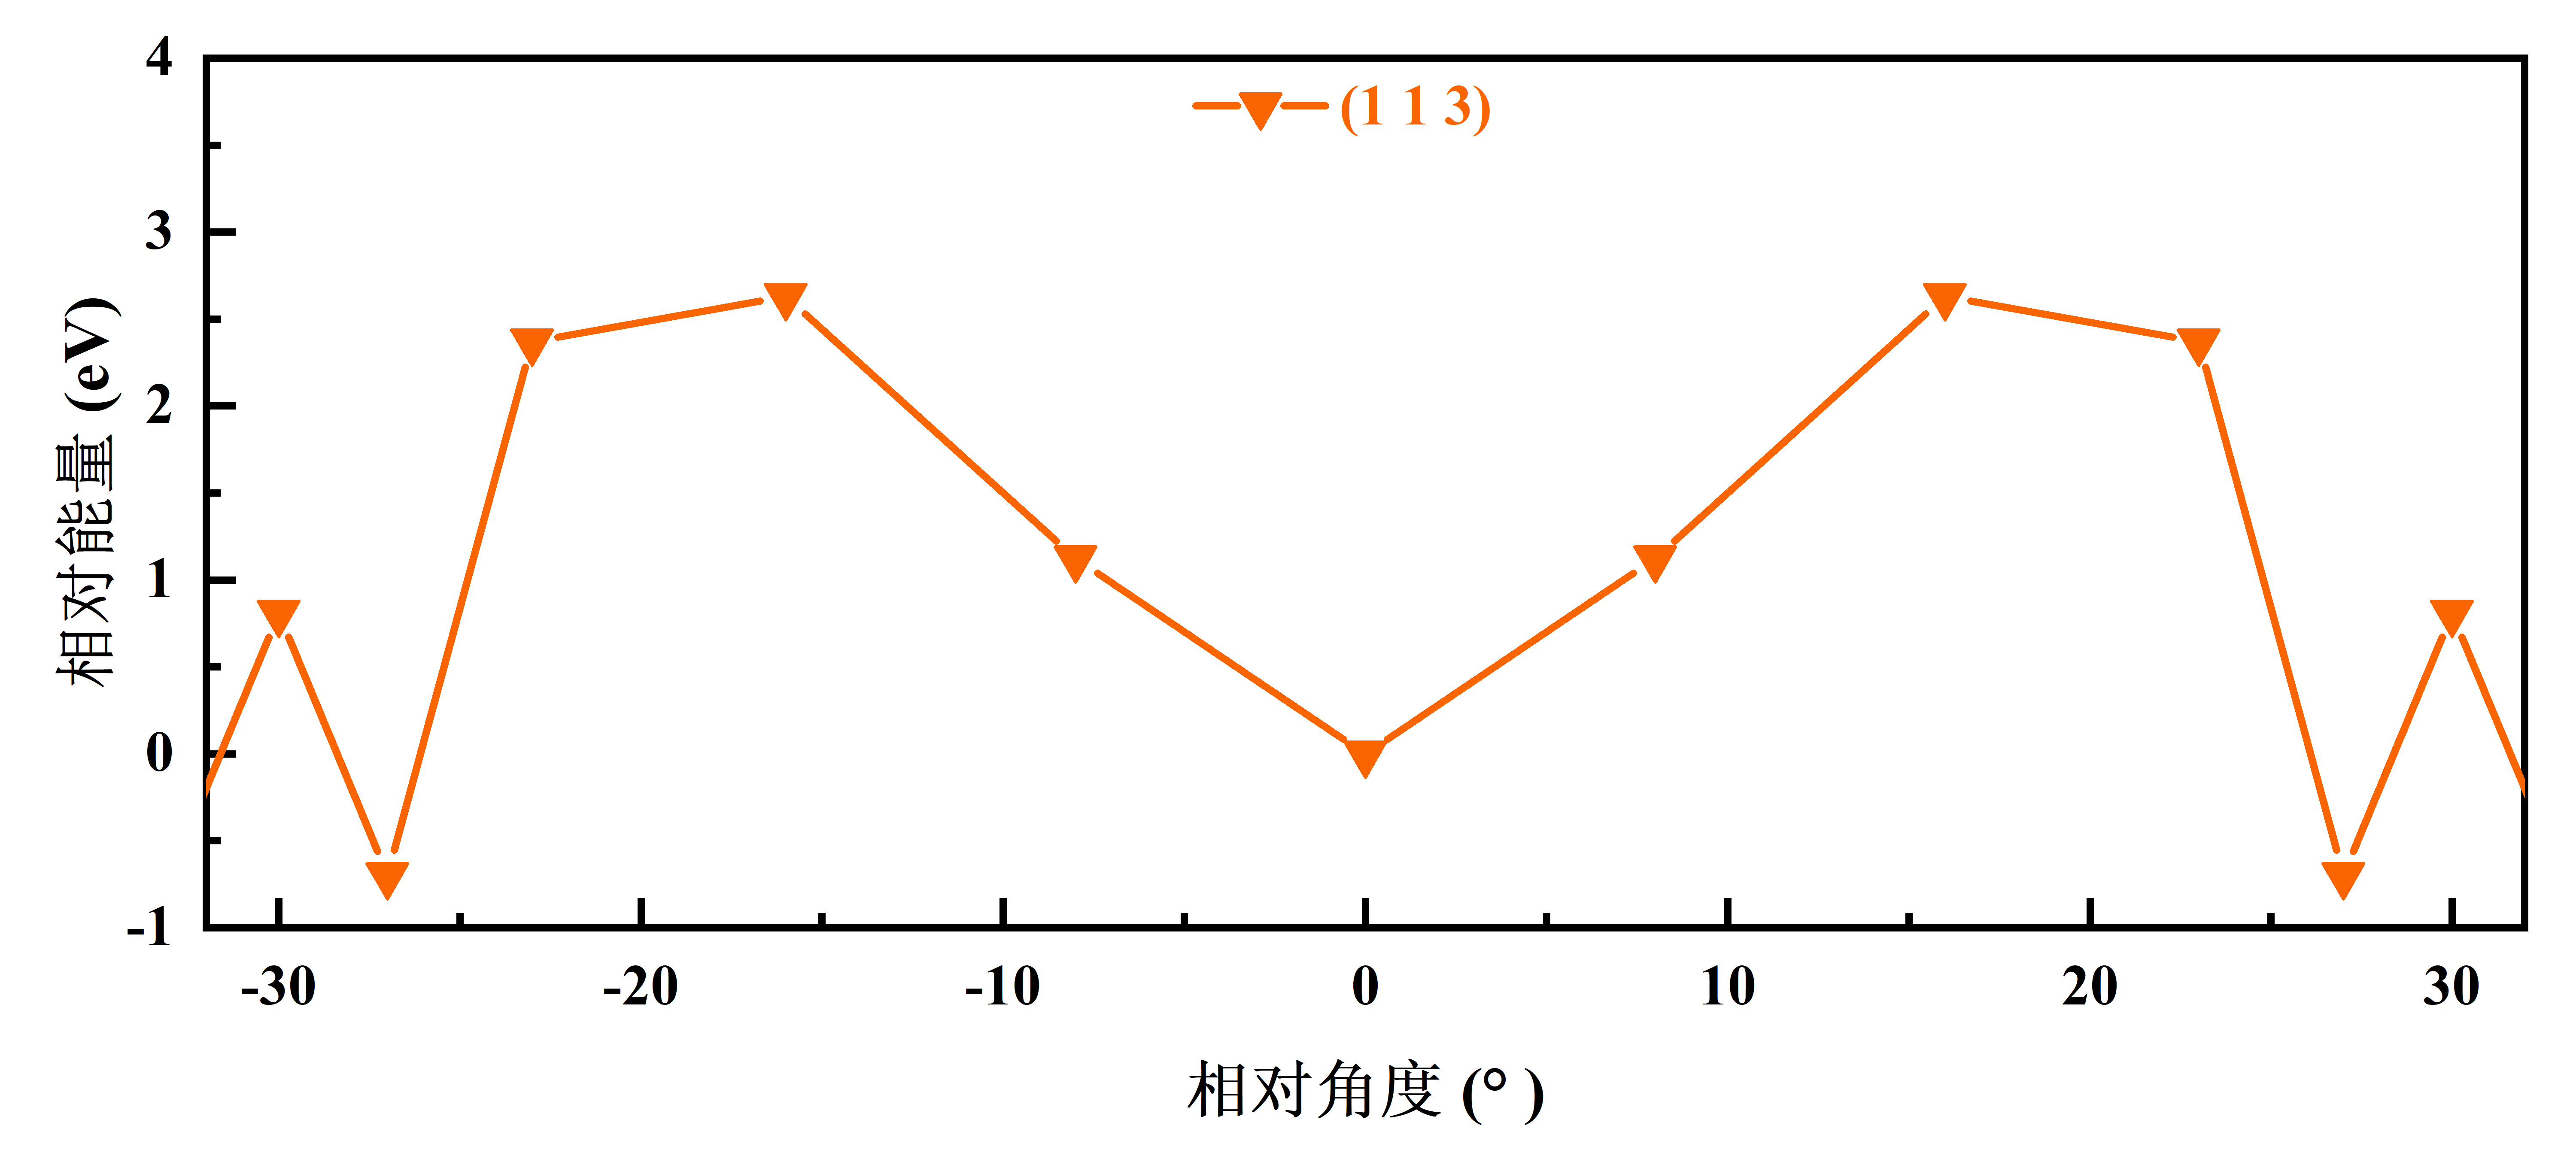
\includegraphics[width=0.8\textwidth]{pic/GO_C24_113_energy.png}
    }
    \caption{铜(113)晶面上石墨烯$\CCluster{24}$团簇的最优生长晶向($\SI{\pm 270}{\degree}$)、原子构型以及各生长角度能量分布图。(a)原子构型侧视图;(b)原子构型俯视图;(c)各生长角度能量分布。图中,碳原子为灰色,铜原子为红色,不同层的铜原子以不同亮度进行区分。}
    \label{GO_C24_113}
\end{figure}

在图\ref{fig:GO_C24_energyDiff_barrier}和表\ref{tab:GO_energyDiff_barrier}中,我们总结了$\rm{(11n)(n \geqslant 1)}$这一系列的铜衬底上石墨烯$\CCluster{24}$团簇的定向生长能量指标。可以看到,在能够实现$\CCluster{24}$团簇定向生长的衬底中,铜(115)晶面具有最高的最优-次优生长角度能量差值,为$\SI{0.64 }{\electronvolt}$。根据热力学的统计定律,我们可以计算$\CCluster{24}$团簇在热平衡状态下处于最优生长角度和次优生长角度的比例$r$\chinesecolon
\begin{equation}
    r=e^{-\frac{\Delta E}{k_{\rm B}T}}
\end{equation}

其中$\Delta E$为两个态之间的能量差,$k_{\rm B}$为玻尔兹曼常数,$T$为温度。对于$\CCluster{24}$团簇在铜(115)晶面的成核生长,取温度$T$为常见的化学气相沉积生长石墨烯的温度$\SI{1300 }{\kelvin}$,我们可以计算得出$\CCluster{24}$团簇处于处于最优生长角度和次优生长角度的比例$r\approx 0.0037$。即在热平衡状态写只有不到$\SI{0.4}{\percent}$的石墨烯$\CCluster{24}$团簇处于非定向生长的状态。而对于最优-次优生长角度差值较低的铜(112)晶面,同样计算可得$\CCluster{24}$团簇在其上生长的$r\approx 0.053$。相比于铜(115)面,铜(112)面的非定向石墨烯畴的比例上升了一个数量级。

进一步考虑$\CCluster{24}$团簇在不同衬底表面从次优生长角度转变至最优生长角度的旋转势垒。在能够实现$\CCluster{24}$团簇定向生长的衬底中,铜(112)晶面具有最低的旋转势垒,为$\SI{1.57 }{\electronvolt}$。铜(115)面紧随其后,为$\SI{2.03 }{\electronvolt}$。更低的旋转势垒可以使$\CCluster{24}$团簇更快得达到热平衡的状态。

\begin{figure}[htb]
    \includegraphics[width=0.8\textwidth]{pic/GO_C24_energyDiff_barrier.png}
    \caption{$\CCluster{24}$团簇在不同衬底表面的次优-最优生长角度能量差(点)和旋转势垒(柱)。能够实现定向生长的衬底以黑点标识,无法实现定向生长的衬底以黑红点标识。}
    \label{fig:GO_C24_energyDiff_barrier}
\end{figure}

综合考虑最优-次优能量差和旋转势垒的情况,我们发现对于$\rm{(11n)(n \geqslant 1)}$这一系列的铜衬底,由于由台阶的存在,石墨烯在能量上会倾向于在台阶的边缘定向生长。虽然铜(113)台面上不重叠的两个最优生长角度会使得石墨烯呈现出不定向生长的趋势,但是由于(113)台面非常高表面能,在实际生长过程中的占比很小。因此我们认为可以使用基于$\rm{(11n)(n \geqslant 1)}$这一系列的指数的多晶铜衬底,尤其是指数接近铜(112)晶面,对石墨烯进行定向生长,从而高效低成本的制备大面积单晶石墨烯。

\begin{table}[htb]
    \caption{石墨烯$\CCluster{24}$团簇在铜$\rm{(11n)(n \geqslant 1)}$衬底上定向生长的最优角度,最优-次优能量差以及旋转势垒}
    \centering
    \begin{tabular}{ccccc}
        \toprule
        铜晶面指数 & 最优生长角度            & 次优生长角度           & 能量差  & 旋转势垒 \\
        \midrule
        (001)      & $\SI{\pm 15 }{\degree}$ & 非定向                 & 非定向                      & 非定向                       \\
        (11X)      & $\SI{0}{\degree}$       & $\SI{\pm 30}{\degree}$ & $\SI{0.56 }{\electronvolt}$ & $\SI{2.56 }{\electronvolt}$  \\
        (117)      & $\SI{0}{\degree}$       & $\SI{\pm 30}{\degree}$ & $\SI{0.43 }{\electronvolt}$ & $\SI{2.91 }{\electronvolt}$  \\
        (115)      & $\SI{0}{\degree}$       & $\SI{\pm 30}{\degree}$ & $\SI{0.63 }{\electronvolt}$ & $\SI{2.07}{\electronvolt}$  \\
        (113)      & $\SI{\pm 27}{\degree}$  & $\SI{0}{\degree}$      & 非定向                      & 非定向                       \\
        (112)      & $\SI{0}{\degree}$       & $\SI{\pm 30}{\degree}$ & $\SI{0.33 }{\electronvolt}$ & $\SI{1.57 }{\electronvolt}$  \\
        (111)      & $\SI{\pm 18 }{\degree}$ & 非定向                 & 非定向                      & 非定向                       \\
        \bottomrule
    \end{tabular}
    \label{tab:GO_energyDiff_barrier}
\end{table}

\section{氧气对化学气相沉积法中石墨烯多层生长的作用}
\label{sec:石墨烯氧蚀刻穿透}
\def\muO#1{\it \mu_{\rm O}^{\rm #1} \it}
\def\halfEOm{\it \frac{1}{2}E_{\rm \cemb{O2}} \it}
\def\EOa{\it E_{\rm O} \it }
\def\Cdis{\rm{\left[C_{dis.}\right]} \it }
\def\Oads{\rm{\left[O_{ads.}\right]} \it }
\def\RateV#1#2{\it \nu_{\rm #1}^{\rm #2} \it }
\def\RateK#1#2{\it{k_{\rm #1}^{\rm #2}} \it }
\def\ReactTime#1#2{\it{t_{\rm #1}^{\rm #2}} \it }

%//TODO mhchem 化学式修改
\subsection{化学气相沉积法中石墨烯生长气氛模拟}
\label{subsec:FLG_gasPhase}
当铜衬底的表面覆盖满石墨烯后,由于铜衬底的对甲烷的催化机制被石墨烯阻挡,石墨烯的生长表现出自限制的效应,使得石墨烯保持单层的形貌。因此,当我们要在覆盖满石墨烯的铜衬底上继续生长双层乃至于多层石墨烯,生长气氛中的甲烷的化学反应动力学过程就变得尤为重要。已有研究者证明,氧气的加入会促进甲烷在气相过程中的裂解,有利于石墨烯第二层的生长\citing{RN1052-2016}。利用气相动力学模拟的方法,我们计算了在引入氧气的情况下常压化学气相沉积系统(APCVD)中化学组分的浓度分布。

首先,我们计算了化学气相沉积过程中石墨烯生长位点的化学组分随时间分布的浓度变化情况(图\ref{fig:FLG_fluent})。依照实验中的生长参数,我们设定氩氧混合气体的流量为$\SI{120}{SCCM}$。其中氩氧混合气中的氧气浓度比例为$\SI{0.4}{\percent}$。模拟环境中其他输入气体的流量参数为$\SI{8}{SCCM}$的纯氢气,$\SI{20}{SCCM}$的甲烷氩气混合气体(其中甲烷的浓度比例为$\SI{1}{\percent}$),$\SI{300}{SCCM}$的纯氩气。我们以含氧混合气体通入反应炉的时间作为模拟的开始时间$\SI{0}{\second}$,反应炉中的初始状态为含有纯氩气作为保护。

\begin{figure}[htb]
    \centering
    \subfloat[]{
        \label{fig:FLG_fluent_C_molConcen}
        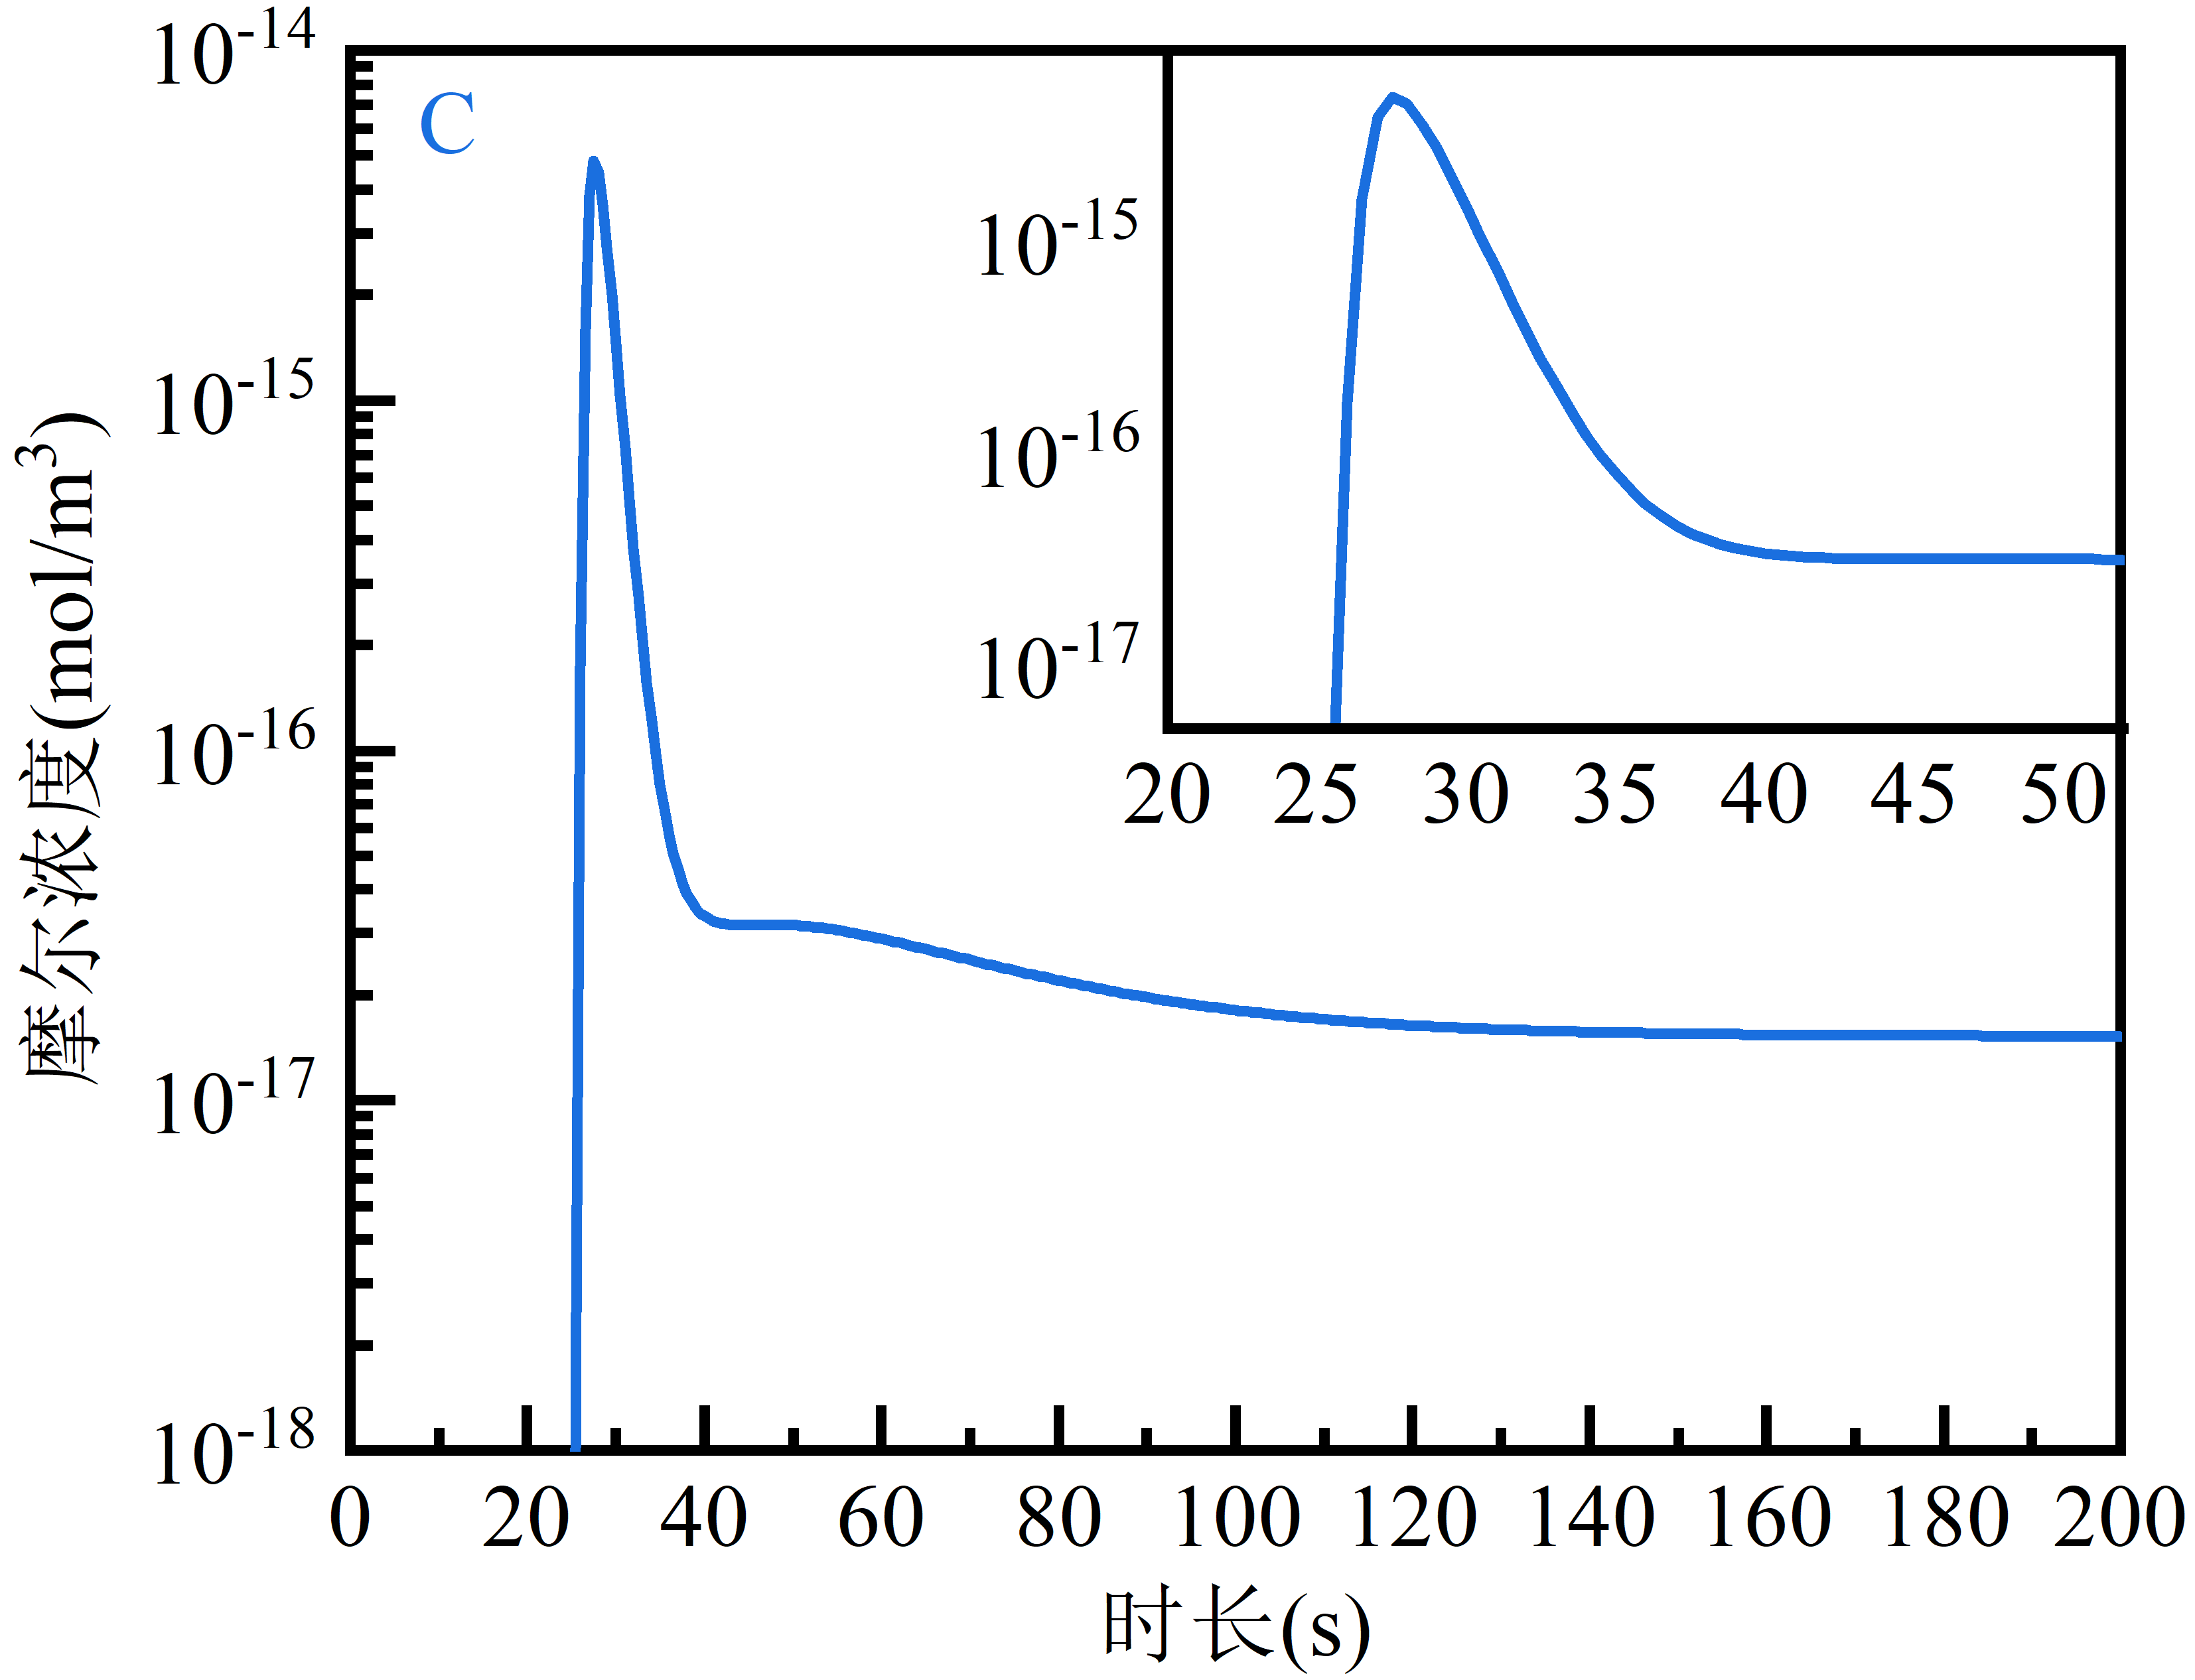
\includegraphics{pic/FLG_fluent_C_molConcen.png}
    }
    \subfloat[]{
        \label{fig:FLG_fluent_O_molConcen}
        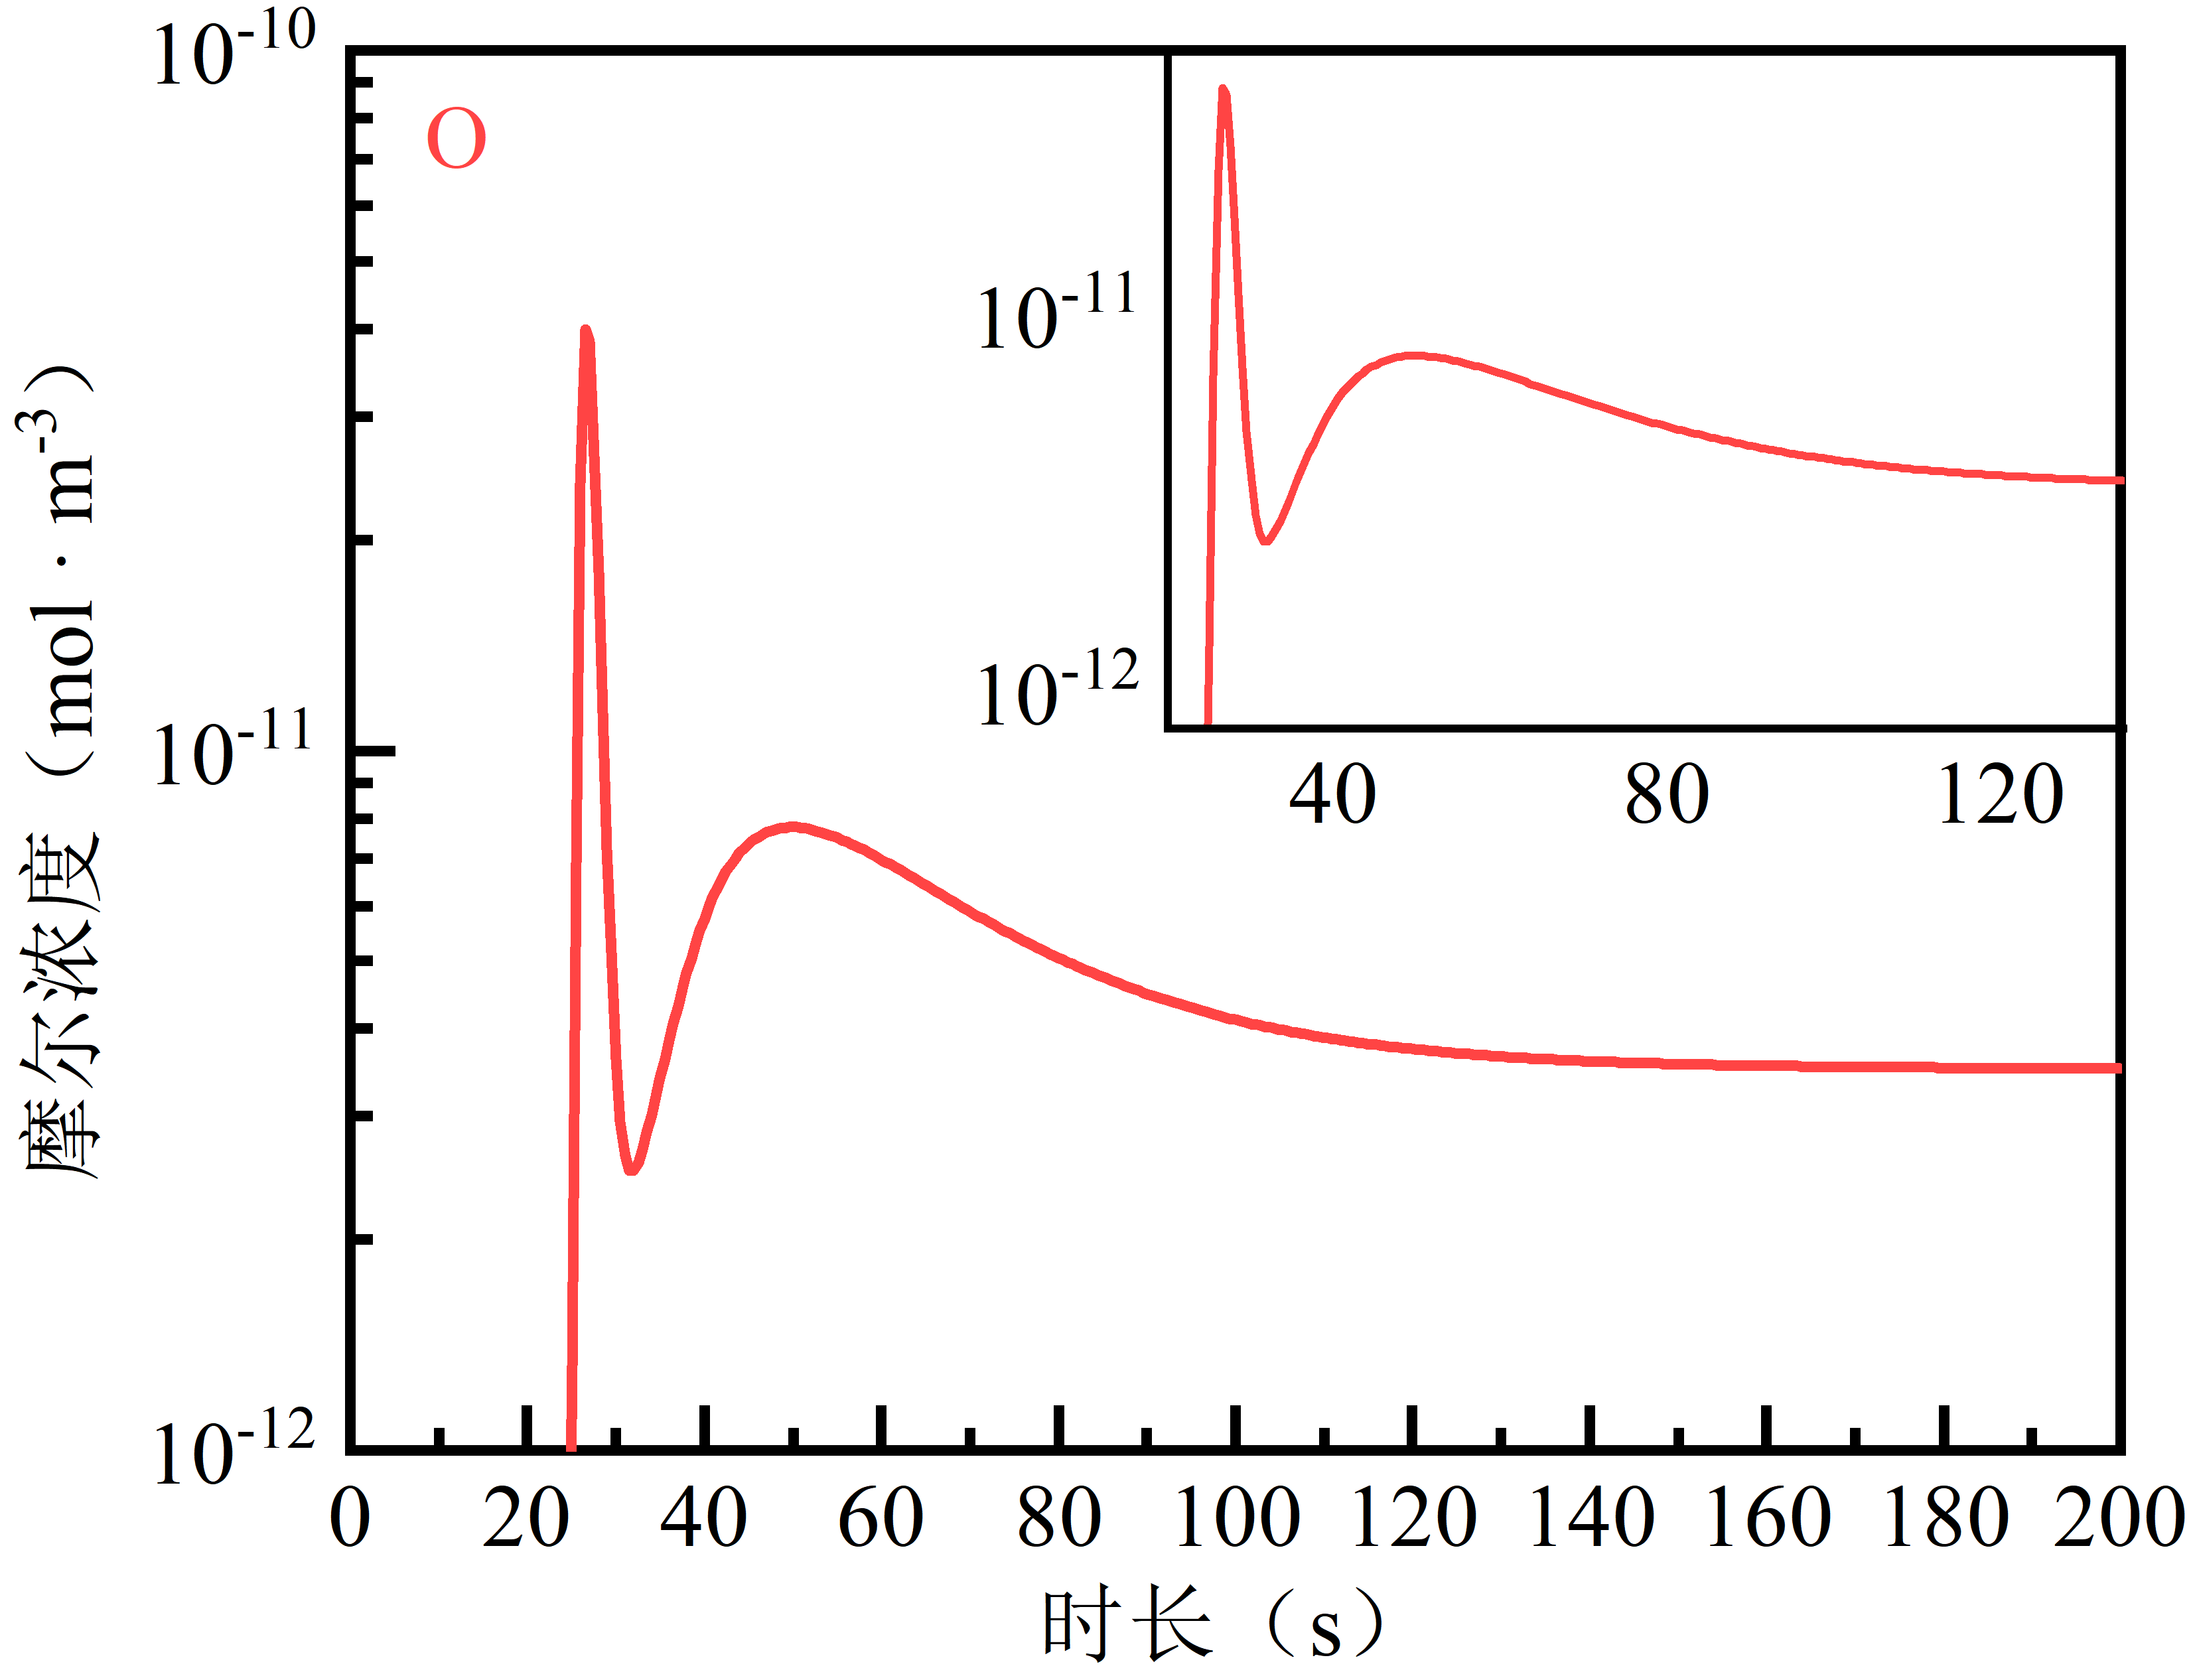
\includegraphics{pic/FLG_fluent_O_molConcen.png}
    }\\[-0.5ex]
    \subfloat[]{
        \label{fig:FLG_fluent_O-C_ratio}
        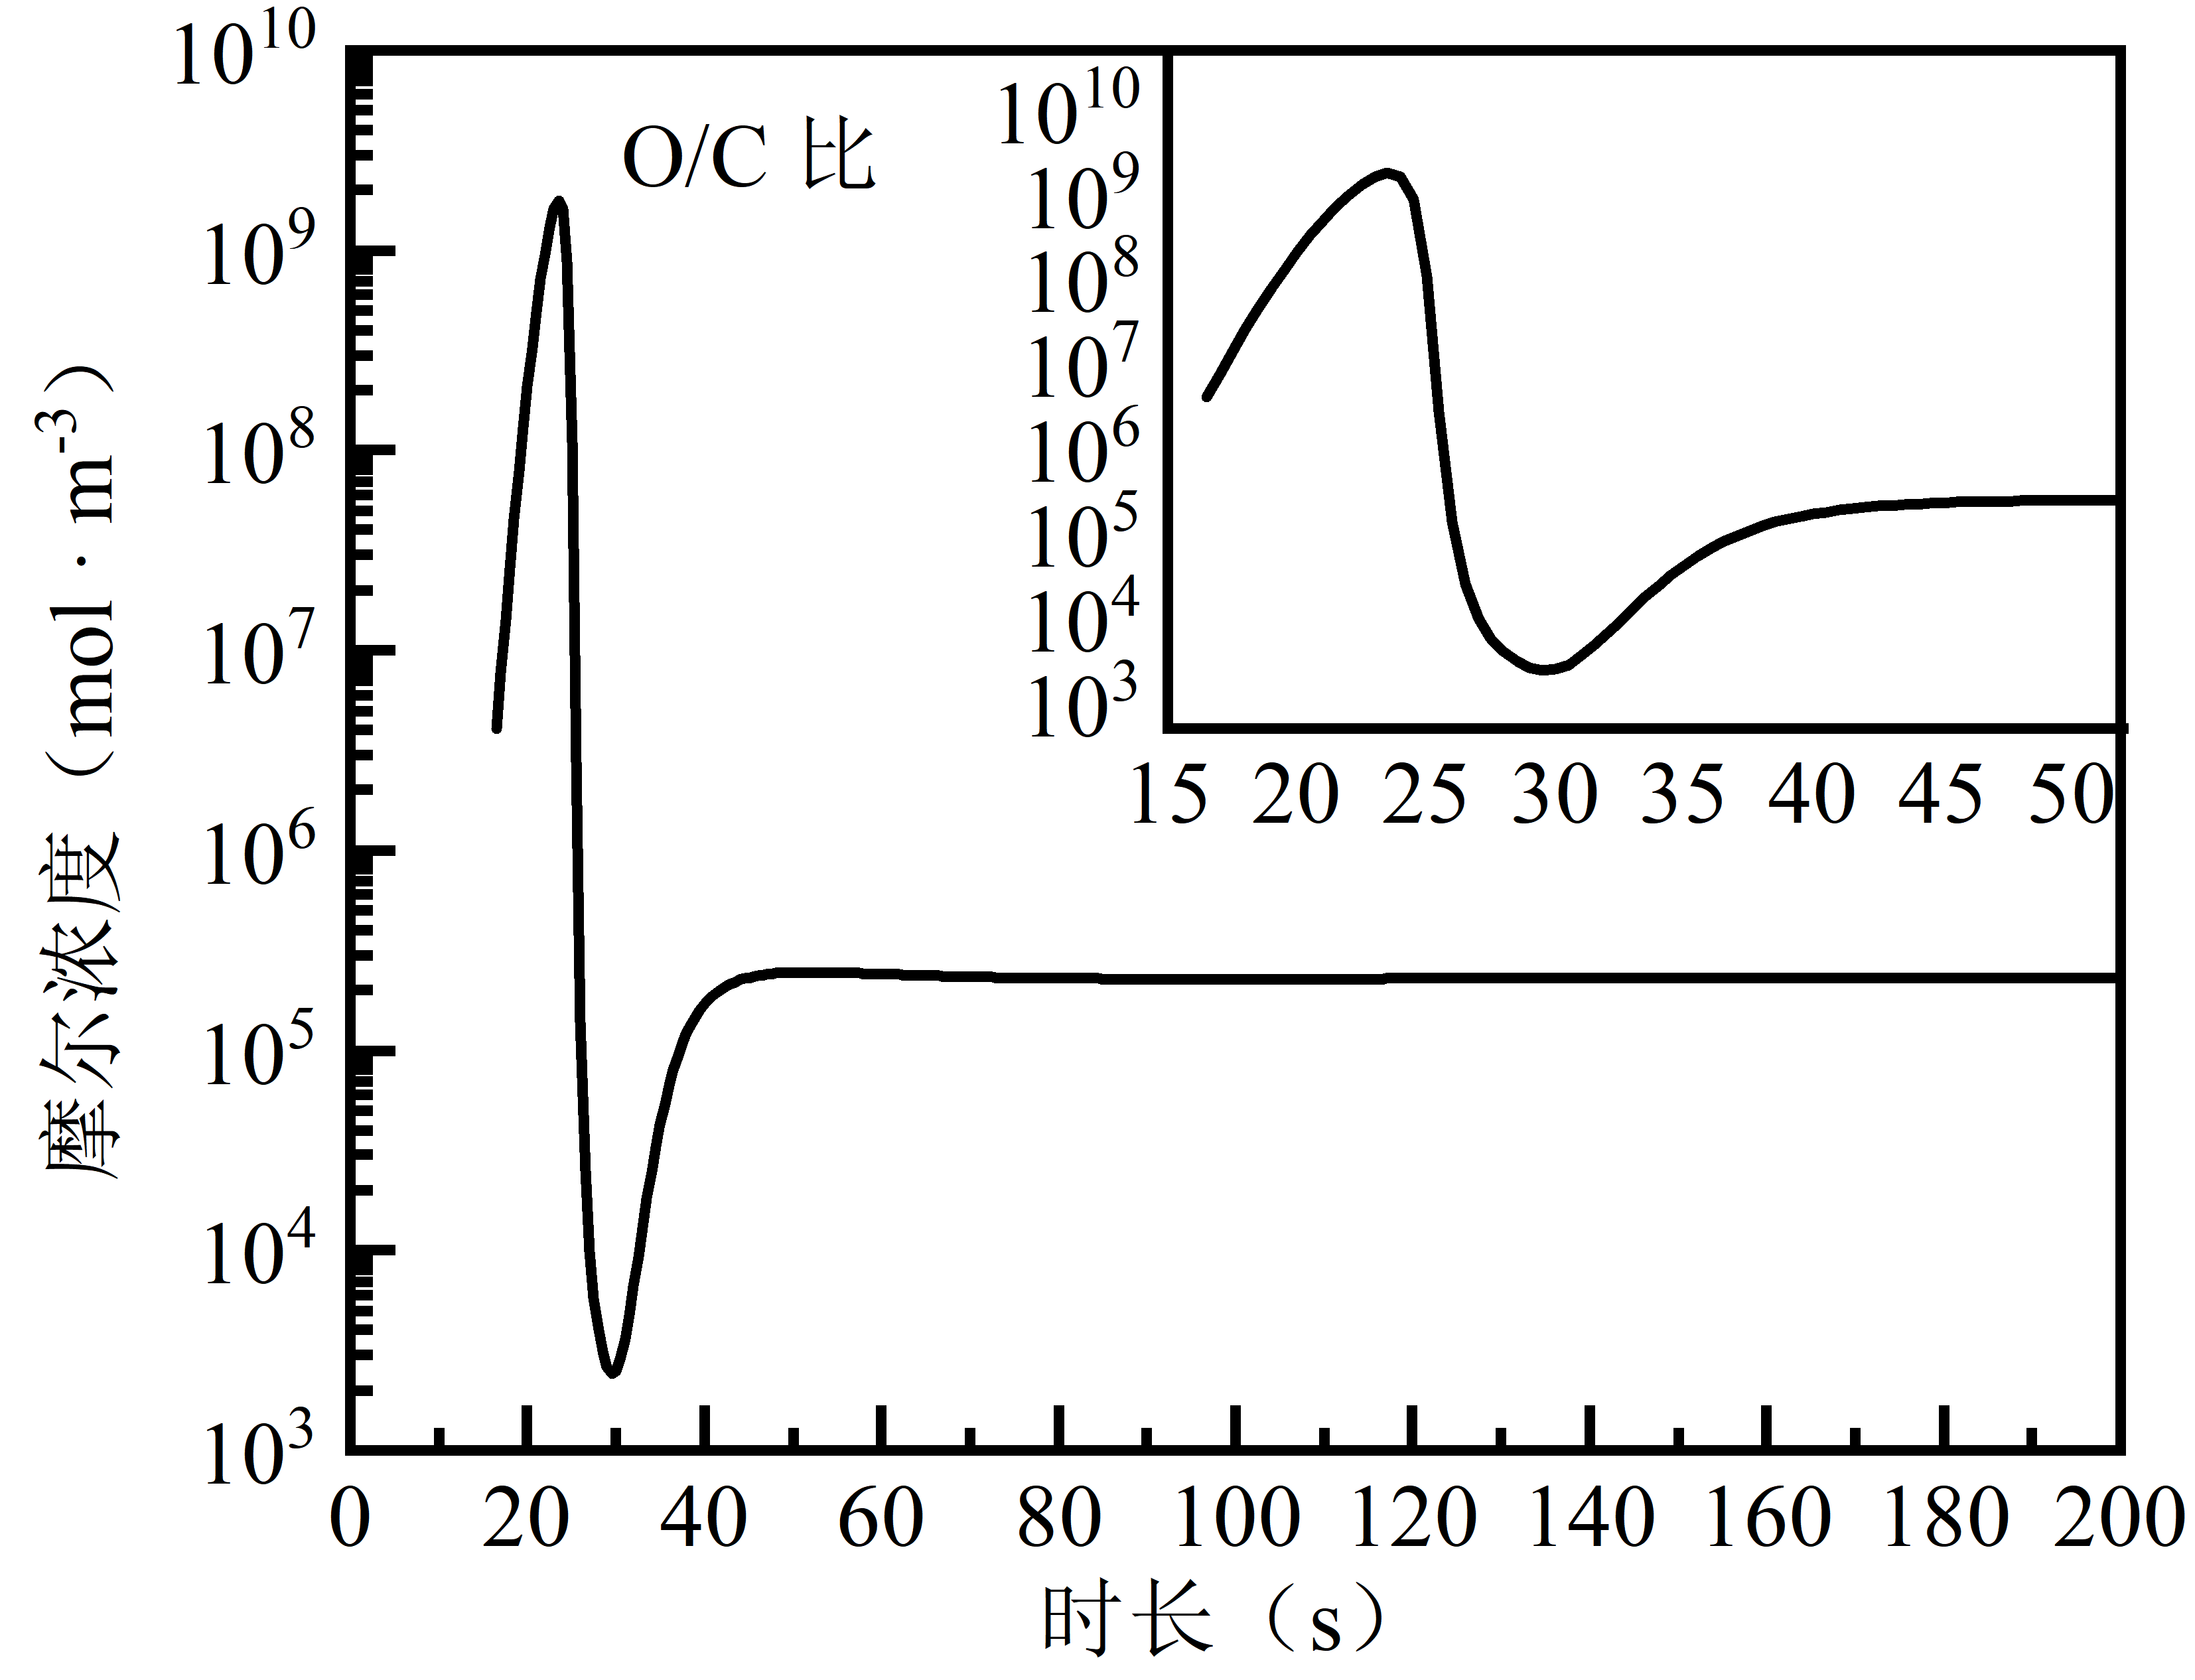
\includegraphics{pic/FLG_fluent_O-C_ratio.png}
    }
    \caption{化学气相沉积过程中石墨烯生长位点的化学组分随时间分布的浓度变化。(a)C自由基浓度(b)O自由基浓度(c)O/C比例。
    }
    \label{fig:FLG_fluent}
\end{figure}

我们使用反应活性最高的C自由基和O自由基作为气相中直接参与石墨烯生长和蚀刻反应的代表反应物。可以看到在常压化学气相沉积的系统内,输入氧气后大约\SI{25}{\second}之后,在石墨烯生长位点开始有明显的甲烷分解反应发生。对于C自由基而言,由于氧气参与并促进甲烷的裂解反应,C自由基的浓度极速上升,最高浓度可达$\SI{4e-15}{\mole\per\cubic\metre}$。随后由于CO、CO2等碳氧化物的生成,C自由基的浓度迅速下降,并在约第\SI{40}{\second}后C自由基的浓度稳定在$\SI{1e-17}{\mole\per\cubic\metre}$附近。而对于O自由基,情况则更为复杂。在$\SI{25}{\second}$时,氧气经过气体输运到达石墨烯生长位点,被迅速加热开始分解成为氧自由基。此时氧自由基的最高浓度最高可达$\SI{3e-11}{\mole\per\cubic\metre}$。随后由于参与甲烷裂解和与氢气的化合反应,氧自由基的浓度下降至$\SI{2e-12}{\mole\per\cubic\metre}$并在产生震荡。氧自由基浓度震荡在约$\SI{50}{\second}$处到达最高值$\SI{8e-12}{\mole\per\cubic\metre}$并逐渐回落至$\SI{3e-12}{\mole\per\cubic\metre}$。考虑到在石墨烯的生长过程中,以C自由基和O自由基为代表的活性物质对于石墨烯的生长和蚀刻作用是同时进行的,因此我们使用O/C比来考察化学气相沉积过程中,通入氩氧混合气后生长气氛中的化合物达到平衡状态所需的时间(图\ref{fig:FLG_fluent_O-C_ratio})。可以看到,在O/C比在通入氩氧混合气的第\SI{45}{\second}后就基本趋于稳定。考虑到实验中生长多层石墨烯通常需要几十分钟乃至几个小时的时间,因此我们可以认为在生长气氛中引入氧气的情况下,石墨烯生长、蚀刻反应所涉及的化学气氛均已达到稳态。由此,我们更加快速高效对生长气氛进行稳态模拟。

图\ref{fig:FLG_chemkin}展示了通入不同流量的氧气情况下石墨烯生长位点的化学组分浓度情况。为了探究前驱体中不同氧气含量对多层石墨烯生长的影响,我们考察了氩氧混合气输入的流量从$\SI{0}{SCCM}$ 到$\SI{500}{SCCM}$时,石墨烯生长气氛中的气相化学反应情况。

\begin{figure}[htb]
    \subfloat[]{
        \label{fig:FLG_chemkin_full}
        \includegraphics[width=0.48\textwidth]{pic/FLG_chemkin_full.png}
    }
    \subfloat[]{
        \label{fig:FLG_chemkin_part}
        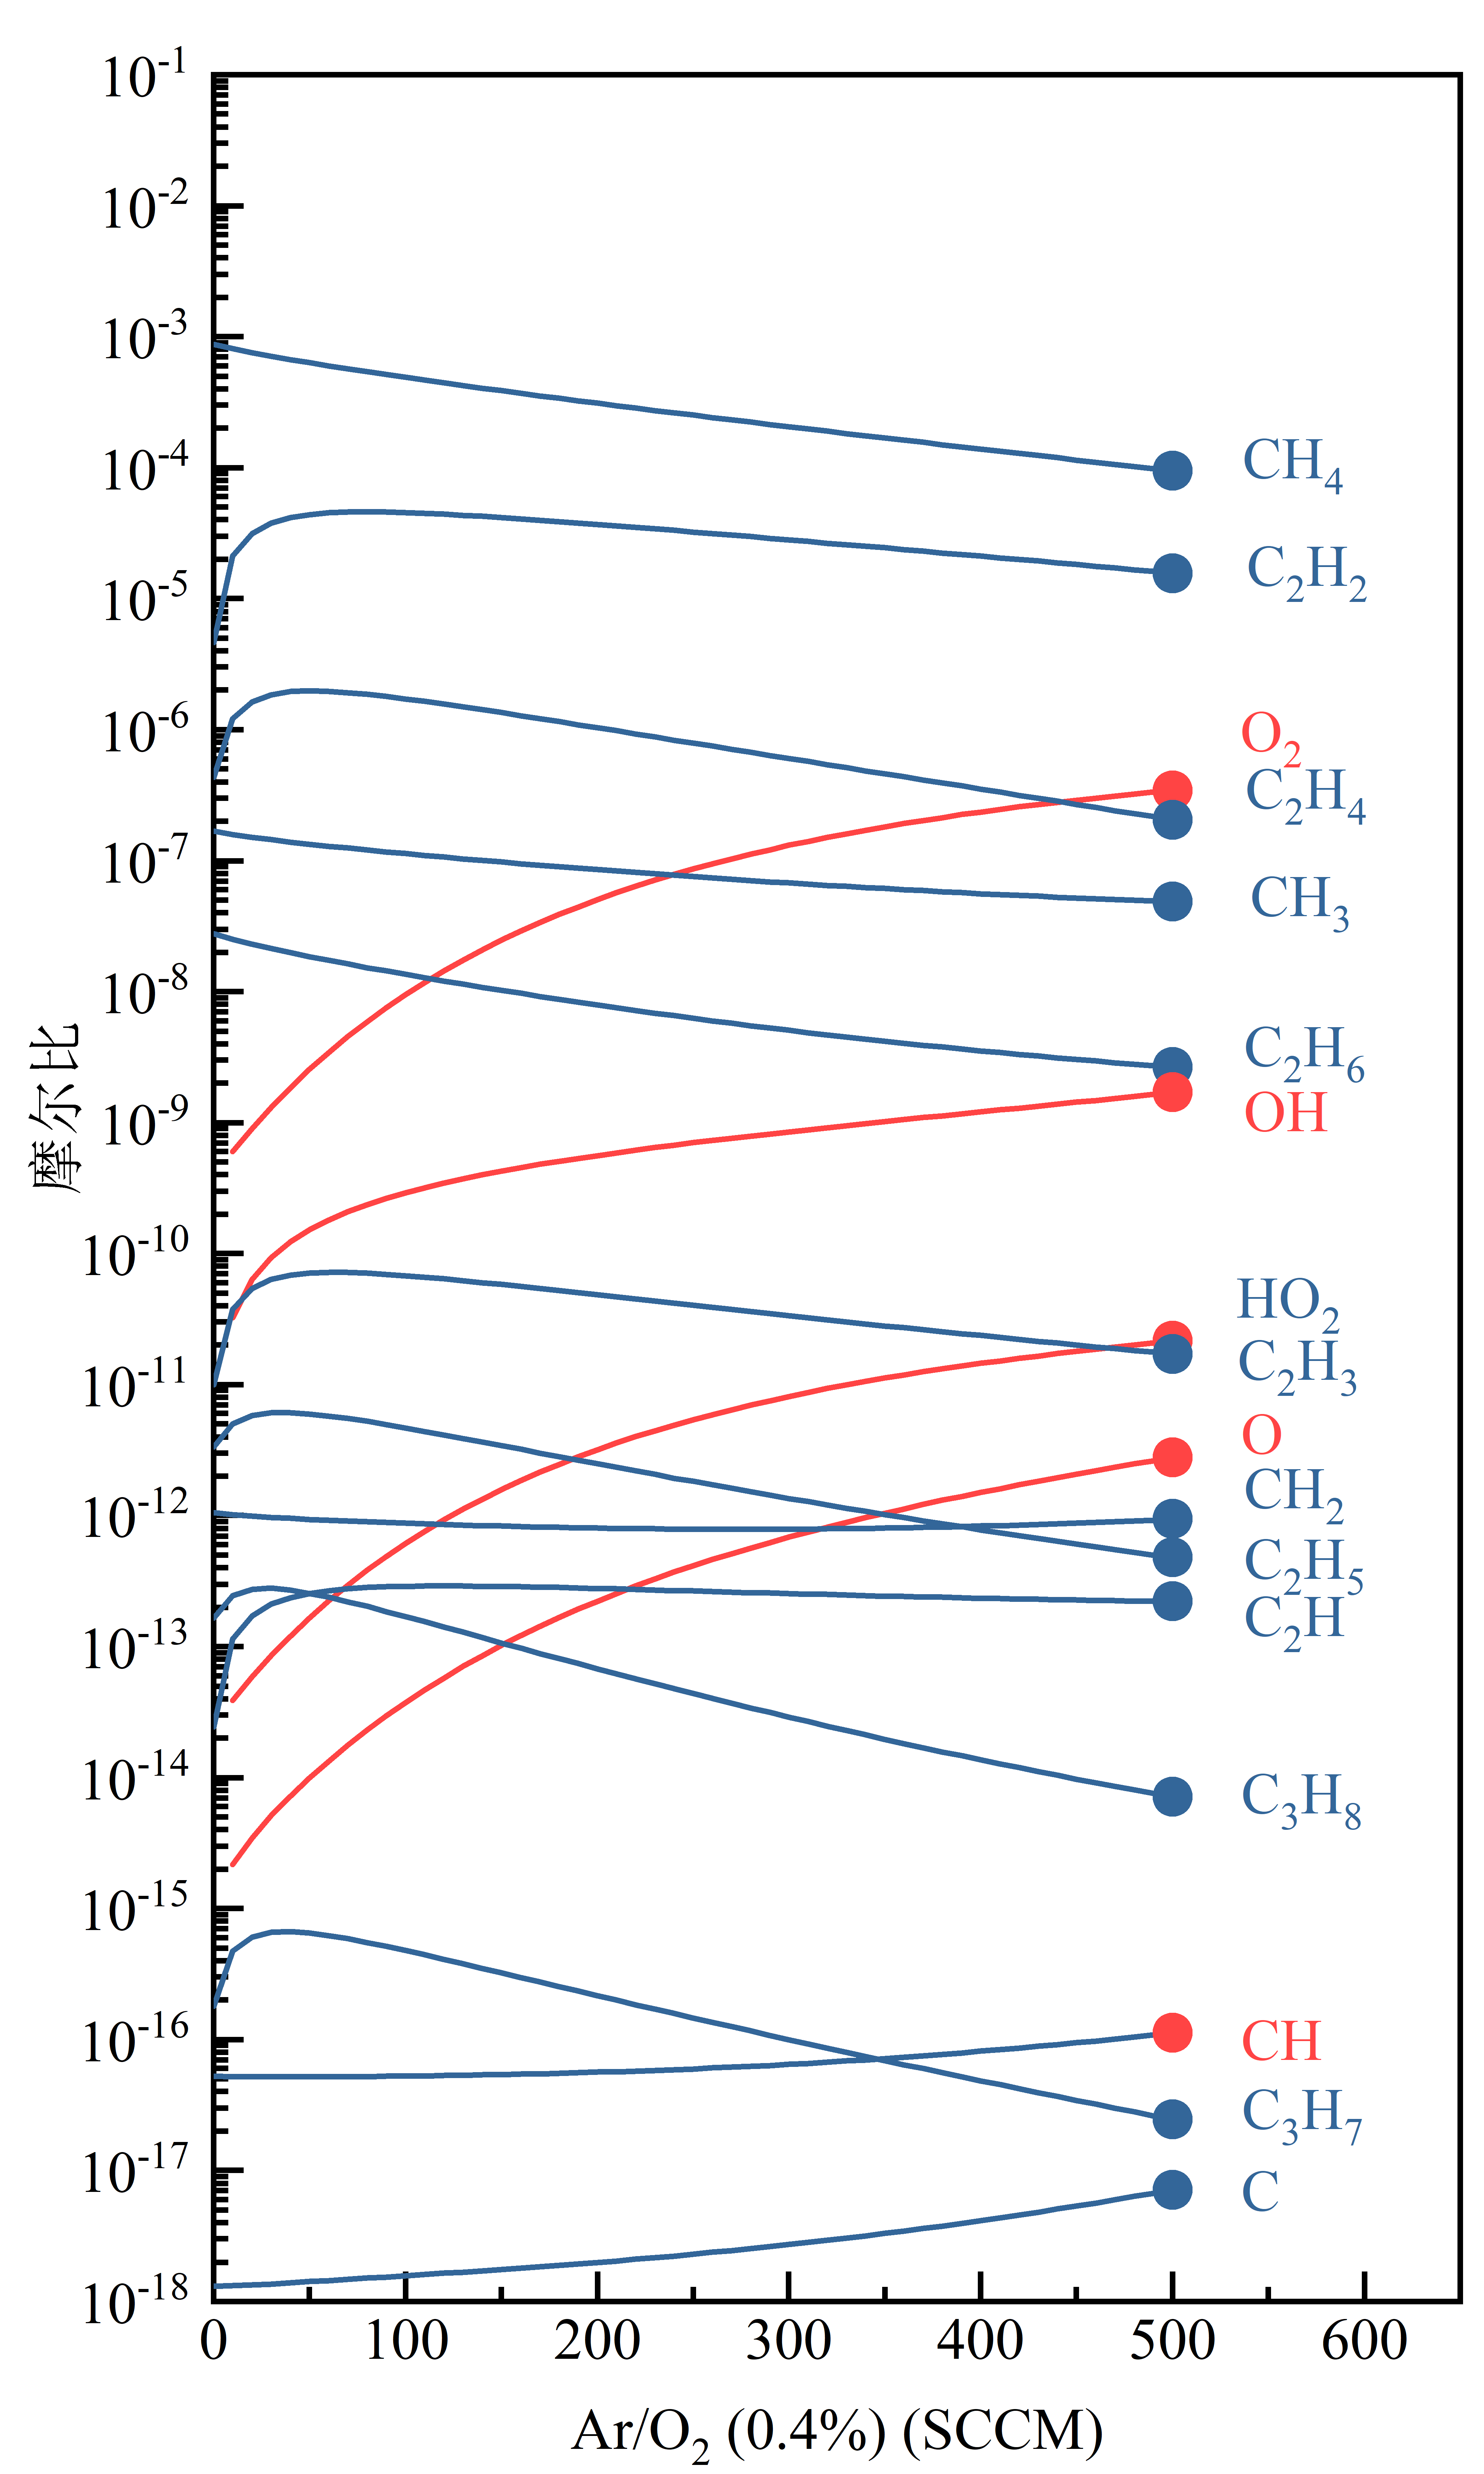
\includegraphics[width=0.48\textwidth]{pic/FLG_chemkin_part.png}
    }
    \caption{生长环境中化学组分浓度分布随着通入氧气流量大小的变化情况。(a)模拟中涉及的所有化合物的浓度分布情况;(b)石墨烯蚀刻物质与生长物质的浓度分布情况}
    \label{fig:FLG_chemkin}
\end{figure}

整体来看,随着通入氧气流量的上升,甲烷的裂解程度也随之上升。甲烷与氧气反应生成大量的一氧化碳和二氧化碳以及种类众多的碳氢氧化合物。而碳氢化合物的浓度随着氧气通入流量的上升呈现出先上升后下降的趋势。氢气的浓度随着更多氧气的通入逐渐下降,但活性氢原子的浓度保持在一个非常稳定的区间。
为了简化分析,在氢-氧-甲烷反应所涉及的所有物质中,我们主要关注那些能够蚀刻石墨烯以及能够为石墨烯生长提供碳源的化合物(图\ref{fig:FLG_chemkin_part})。其中,在本章中所考虑的蚀刻物质包括氧自由基、氢氧化物和氧气,生长物质包括活性炭自由基,碳氢化合物等。

对于蚀刻物质,我们发现随着氧气通入量的上升,O、OH以及$\cemb{HO2}$的浓度急剧上升。以氧自由基为例,活性氧自由基的浓度在氩氧混合气的输入流量为$\SI{5}{SCCM}$时约为$\SI{2e-15}{}$。在氩氧混合气的输入流量为$\SI{500}{SCCM}$时,氧自由基在气氛中的浓度提升至$\SI{3e-2}{}$,大约提升了三个数量级。而对于$\cemb{OH}$和$\cemb{HO2}$,二者的浓度随着氩氧混合气的输入流量的上升也有两到三个数量级的浓度提升。

而气氛中的生长物质随着氧气通入量的上升呈现出了了非单调的变化。氧气能够促进甲烷的裂解反应,因此气氛中的C和CH的浓度得以缓慢上升,作为甲烷裂解反应物和中间产物的$\cemb{CH4}$,$\cemb{CH3}$,$\cemb{CH2}$则缓慢下降。而其他碳氢化合物在氧气通入量逐渐上升的情况下大部分呈现出先上升后下降的浓度趋势。
\subsection{氧对多层石墨烯的穿透蚀刻机制}
\label{subsec:FLG_Oetch}

考虑到蚀刻物质中$\cemb{O}$、$\cemb{OH}$、$\cemb{HO2}$以及$\cemb{O2}$等物质都对石墨烯具有一定的蚀刻作用,且各蚀刻物质之间的浓度较为接近。为了探究石墨烯在含氧化学气相沉积环境下的蚀刻过程,我们引入氧原子的化学势$\muO{}$来代表生长气氛中蚀刻物质的整体反应活性。因此,化学势$\muO{}$的变化范围为$\halfEOm$ 至 $\EOa$,对应于氧原子在氧气分子($\cemb{O2}$)内的能级水平和氧原子在氧自由基($\cemb{O}$)中的能级水平。随着在蚀刻石墨烯的反应中涉及的高活性蚀刻物质(如氧自由基O)浓度的上升,化学势$\muO{}$逐渐上升并接近$\EOa$,同时伴随着更多的石墨烯被蚀刻。

随后,我们利用密度泛函理论,在$\muO{}$的框架内计算了氧原子蚀刻石墨烯的反应能$\Delta E$。
\begin{equation}
    \Delta E = E_{\rm product} - E_{\rm initial} - \muO{}
\end{equation}
其中,$E_{\rm product}$和 $E_{\rm initial}$分别为各反应步骤中生成物和反应物的能量。

在以铜为衬底的化学气相沉积石墨烯生长法中,当铜的表面被单层的石墨烯覆盖满后,石墨烯多层的生长由于自限制效应而趋近于停止。此时的石墨烯-铜衬底界面处存在大量的游离碳。这些游离碳在石墨烯-铜衬底的界面处扩散,成核,形成少量的石墨烯多层点。从热力学的角度看,石墨烯多层点的大小于游离碳的浓度$\Cdis$处于平衡状态。当游离碳的浓度$\Cdis$上升时,处于石墨烯-铜衬底的界面处的石墨烯多层点的成核密度上升、面积扩大。当游离碳的浓度$\Cdis$下降时,石墨烯多层点开始分解,面积缩小。

从密度泛函理论的计算结果来看(图\ref{fig:FLG_DFT_Oetch}),无论有无游离碳,氧原子都可以在石墨烯上吸附,并且吸附的反应能相近。对于氧气来说,由于在石墨烯上吸附需要进行裂解,因此当$\muO{}=\halfEOm$时,氧原子在界面游离碳上方的石墨烯上的吸附能约为$\SI{-0.35}{\electronvolt}$,在纯石墨烯的表面吸附能约为$\SI{-0.28}{\electronvolt}$。而对于氧自由基而言,其可以在石墨烯上直接吸附,相应的吸附步骤的反应能也会下降很多。计算显示当$\muO{}=\EOa$时,氧原子在界面游离碳上方的石墨烯上的吸附能约为$\SI{-3.63}{\electronvolt}$,在纯石墨烯上的吸附能约为$\SI{-3.56}{\electronvolt}$。

\begin{figure}[htb]
    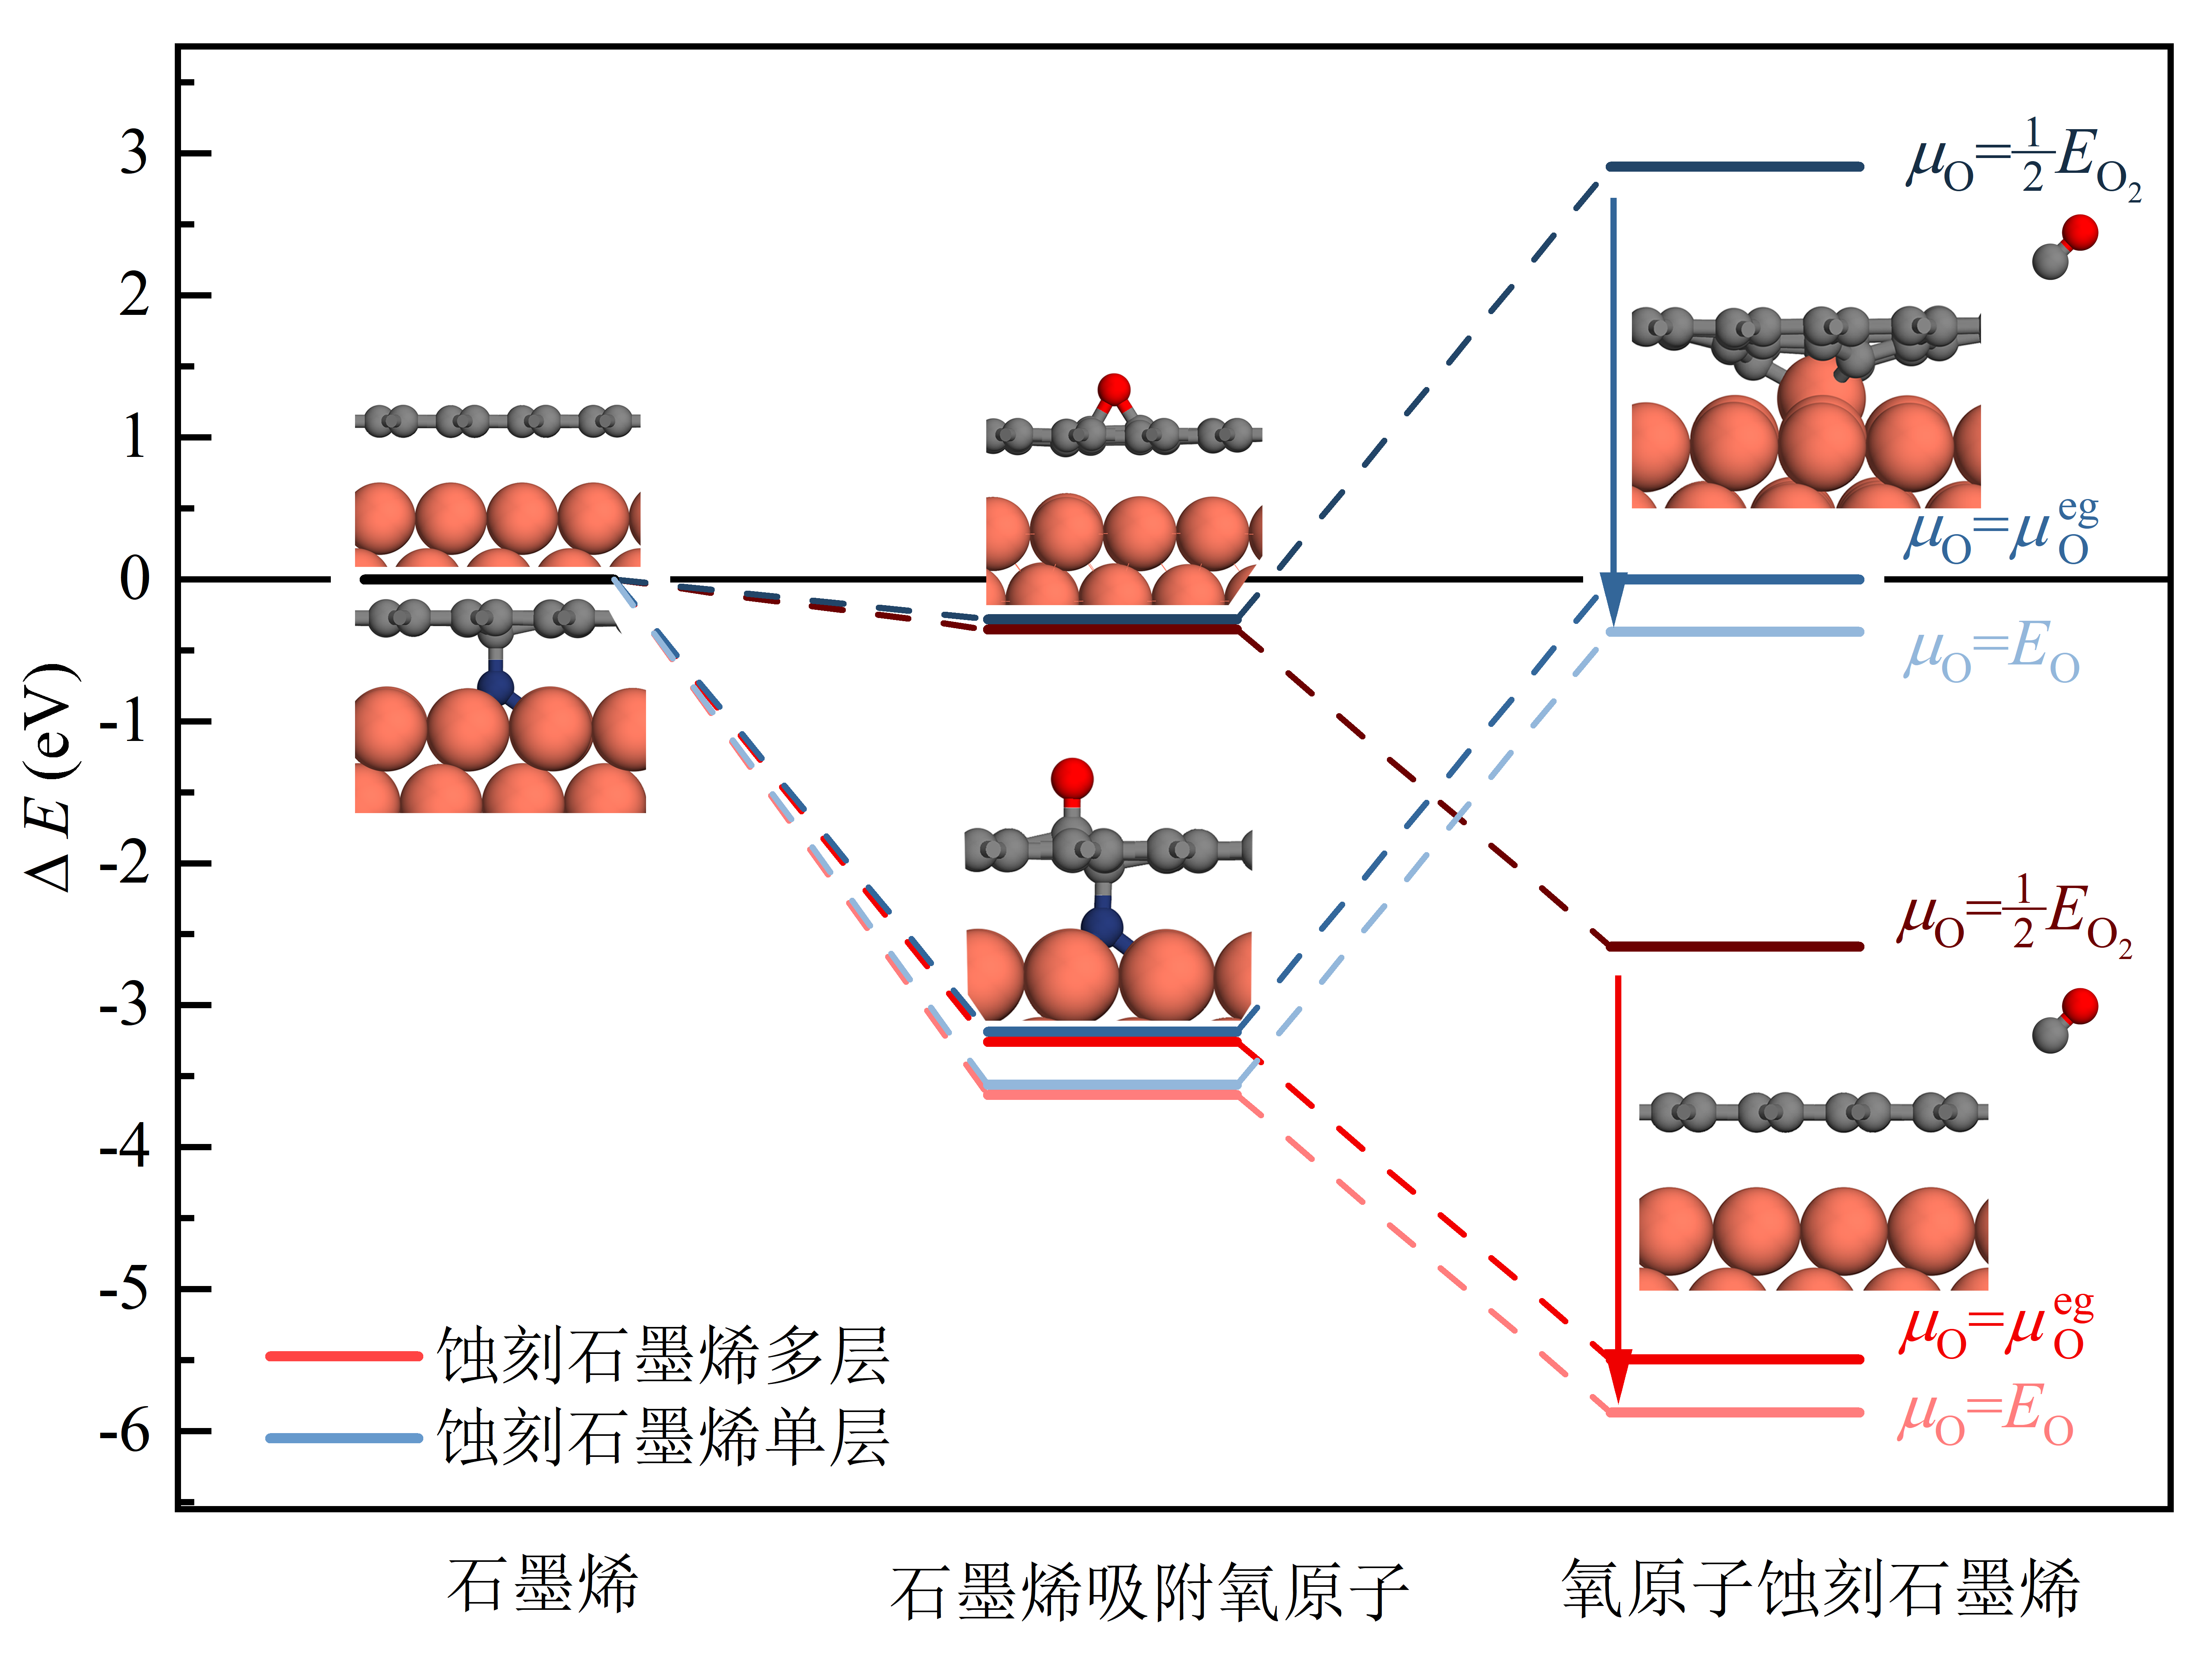
\includegraphics{pic/FLG_DFT_Oetch.png}
    \caption{
        石墨烯多层以及石墨烯单层在含氧环境下的蚀刻。$\muO{eg}$为氧蚀刻石墨烯单层时的平衡化学势。图中,铜原子、碳原子、氧原子、氢原子分别使用橙色、灰色、红色和白色标识。
    }
    \label{fig:FLG_DFT_Oetch}
\end{figure}

氧原子吸附在石墨烯上后,和石墨烯表面的碳原子发生反应,生成非常稳定的\cemb{CO}。同时,当界面游离碳存在的时候,石墨烯上被氧原子蚀刻而成的碳空位能够被游离碳修复。这种类似于交换作用的机理使得环境中的氧原子能够通过蚀刻石墨烯单层的方式减少界面游离碳的浓度$\Cdis$,进而导致石墨烯多层点的蚀刻。计算显示,氧原子在游离碳上方的石墨烯位点蚀刻石墨烯形成\cemb{CO}的反应在所有考虑的氧原子能级$\muO{}$下都为放热反应,在$\muO{}=\halfEOm$时反应能$\Delta E=\SI{-2.59}{\electronvolt}$;在$\muO{}=\EOa$时反应能$\Delta E=\SI{-5.87}{\electronvolt}$。这意味着即使环境中只存在少量的氧气($\muO{} \approx \halfEOm$),生长气氛中的氧就能够通过蚀刻石墨烯单层和游离碳的交换作用对界面处的石墨烯多层进行蚀刻。

当界面处的石墨烯多层被完全蚀刻、游离碳的浓度$\Cdis$也被环境中的氧消耗至零时,氧气与石墨烯单层表面碳原子反应产生的碳空位无法被修复,在石墨烯表面产生高能态的单空位缺陷(Single vacancy, SV)。空位缺陷的产生会极高的抬升氧原子蚀刻石墨烯单层的反应能。导致的结果是只有当环境中氧原子的能级水平提高至接近氧自由基的能级$\EOa$时,蚀刻反应才能够从吸热反应变为放热反应,此时的$\muO{} \leqslant  \muO{eg}  $,才能够进一步对石墨烯单层进行蚀刻。$\muO{eg}$为氧蚀刻石墨烯单层时的平衡化学势。因此,对于石墨烯单层的蚀刻需要通入更高流量的氧气以抬高生长气氛中氧的反应活性。

\subsection{氧对多层石墨烯的穿透生长机制}
\label{subsec:Opene}
在第\ref{subsec:FLG_gasPhase}章中,我们模拟了引入不同流量的氧气的情况下石墨烯生长位点的化合物浓度分布情况。对于生长物质,我们发现\cemb{C2H2}分子的摩尔浓度相比于其他的生长物质的浓度高出多个数量级。因此我们考虑将\cemb{C2H2}分子作为本章的主要研究对象,探究其对于石墨烯多层生长的影响。

首先,我们通过密度泛函理论计算,研究\cemb{C2H2}在石墨烯表面的吸附机理(图\ref{fig:FLG_DFT_C2H2toCHO})。对于无氧生长气氛下的石墨烯,我们的计算结果显示\cemb{C2H2}在其上的吸附反应是吸热的,吸附能为$\SI{0.11}{\electronvolt}$。
这一结果和已有的研究吻合\citing{RN248-2014}。吸热的吸附过程说明\cemb{C2H2}较难在纯石墨烯上吸附,因此也较难对石墨烯多层点的生长产生作用。在有氧的生长气氛下,在\ref{subsec:FLG_Oetch}章中,我们以及证明了生长气氛中的氧在能量上很容易在石墨烯的表面形成吸附氧原子。当石墨烯的表面存在吸附氧原子时,进一步的计算显示气氛中的\cemb{C2H2}可以与吸附氧原子反应,在石墨烯的表面形成\cemb{C2H2O}。这一步骤的反应能下降为$\SI{-1.54}{\electronvolt}$。随后,石墨烯表面吸附的\cemb{C2H2O}能够进一步和氧反应,形成更为稳定的\cemb{C2H2O2}。\cemb{C2H2O2}在石墨烯的表面可以分解成为两个分离的\cemb{CHO},进一步降低体系能量。在反应过程中,仅有\cemb{C2H2O2}分解为石墨烯表面相邻的\cemb{CHO}(图\ref{fig:FLG_DFT_C2H2toCHO},G-2HCO)过程中有小至$\SI{0.027}{\electronvolt}$的反应能上升,其余过程均为放热反应。因此我们可以,在生长气氛中引入氧气的情况下,气氛中的\cemb{C2H2}可以大量的在石墨烯的表面吸附、分解成为同样吸附在石墨烯表面的\cemb{CHO}。

\begin{figure}[htb]
    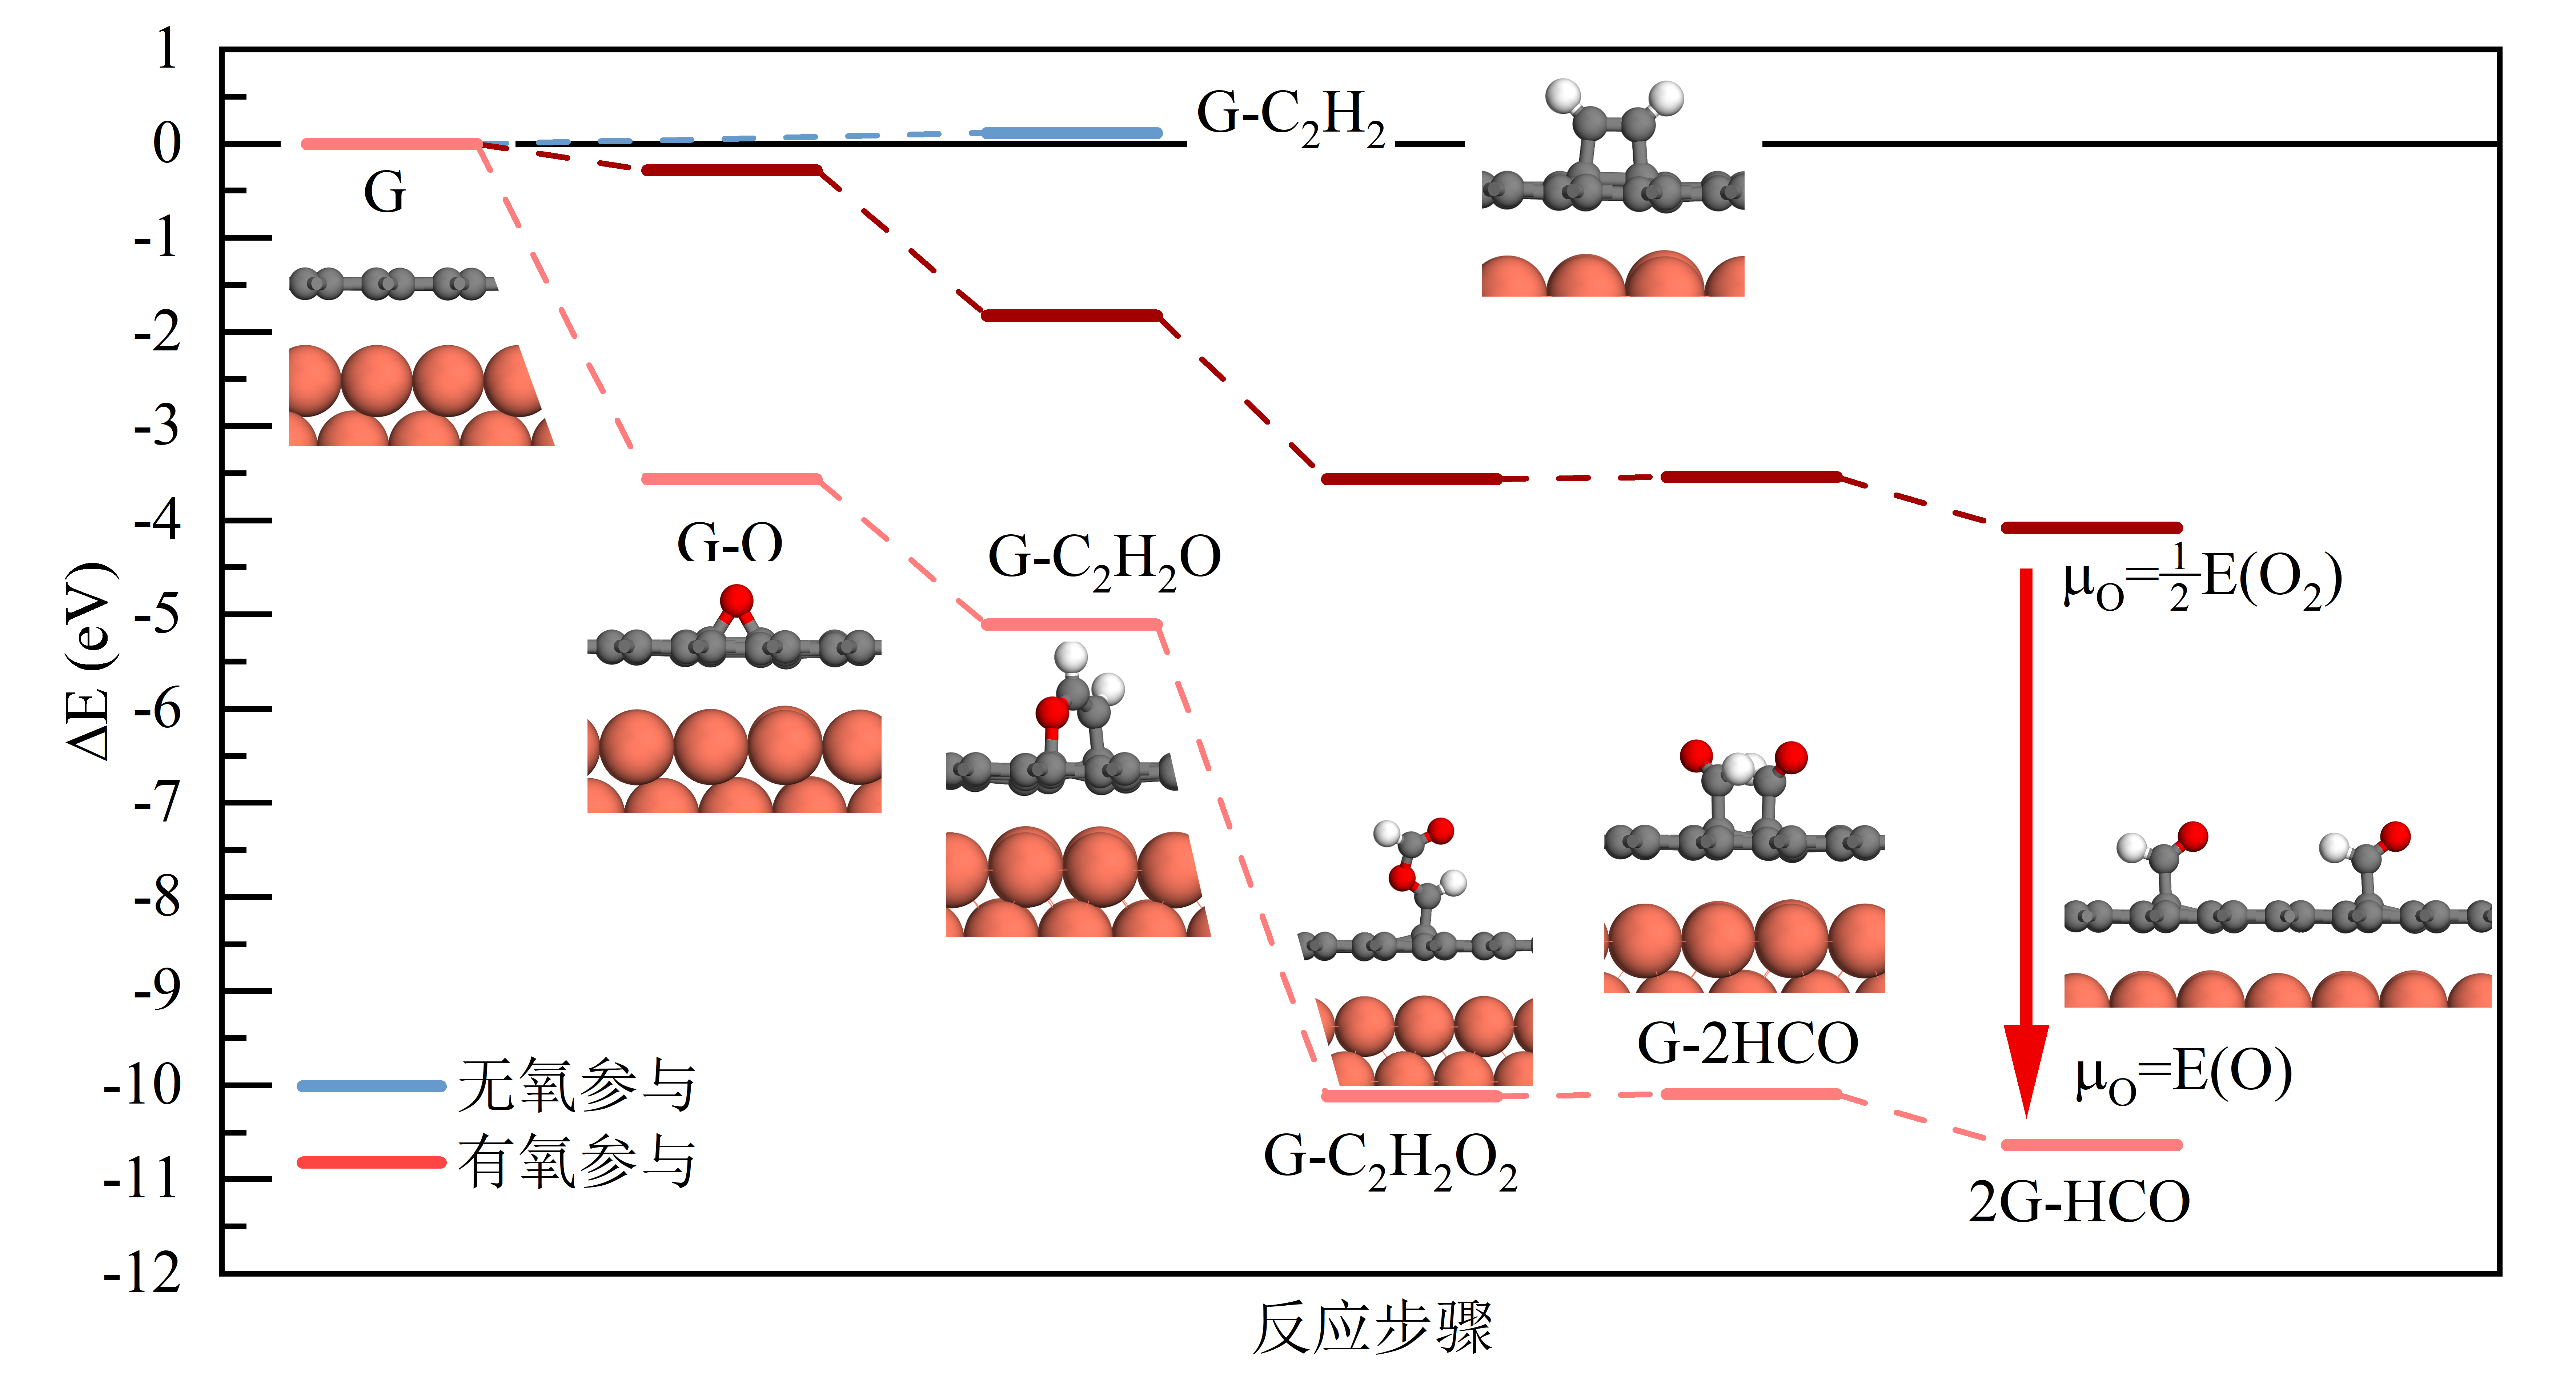
\includegraphics{pic/FLG_DFT_C2H2toCHO.png}
    \caption{氧辅助\cemb{C2H2}在石墨烯表面沉积、分解为\cemb{CHO}。图中,铜原子、碳原子、氧原子、氢原子分别使用橙色、灰色、红色和白色标识。}
    \label{fig:FLG_DFT_C2H2toCHO}
\end{figure}

先前的研究表明,碳自由基以及碳氢化合物(\cemb{CH_x})等物质能够通过穿透的方式,在已生长的石墨烯的下方生长石墨烯多层\citing{RN248-2014}。由于碳自由基在生长气氛中非常低的浓度,已经环境中较高的氢自由基浓度,我们选择\cemb{CH}作为代表化合物考察碳自由基以及碳氢化合物在含氧的生长气氛下对于石墨烯的穿透生长作用。在图\ref{fig:FLG_DFT_CHpene}中,我们计算了石墨烯表面吸附的\cemb{CH}在有氧和无氧的气氛下可能的穿透反应路线。计算结果显示在无氧的气氛下,\cemb{CH}能够很好得在石墨烯得表面吸附并且通过穿透作用形成界面游离碳原子($\rm G-C_{inter}-H$)。

\begin{figure}[htb]
    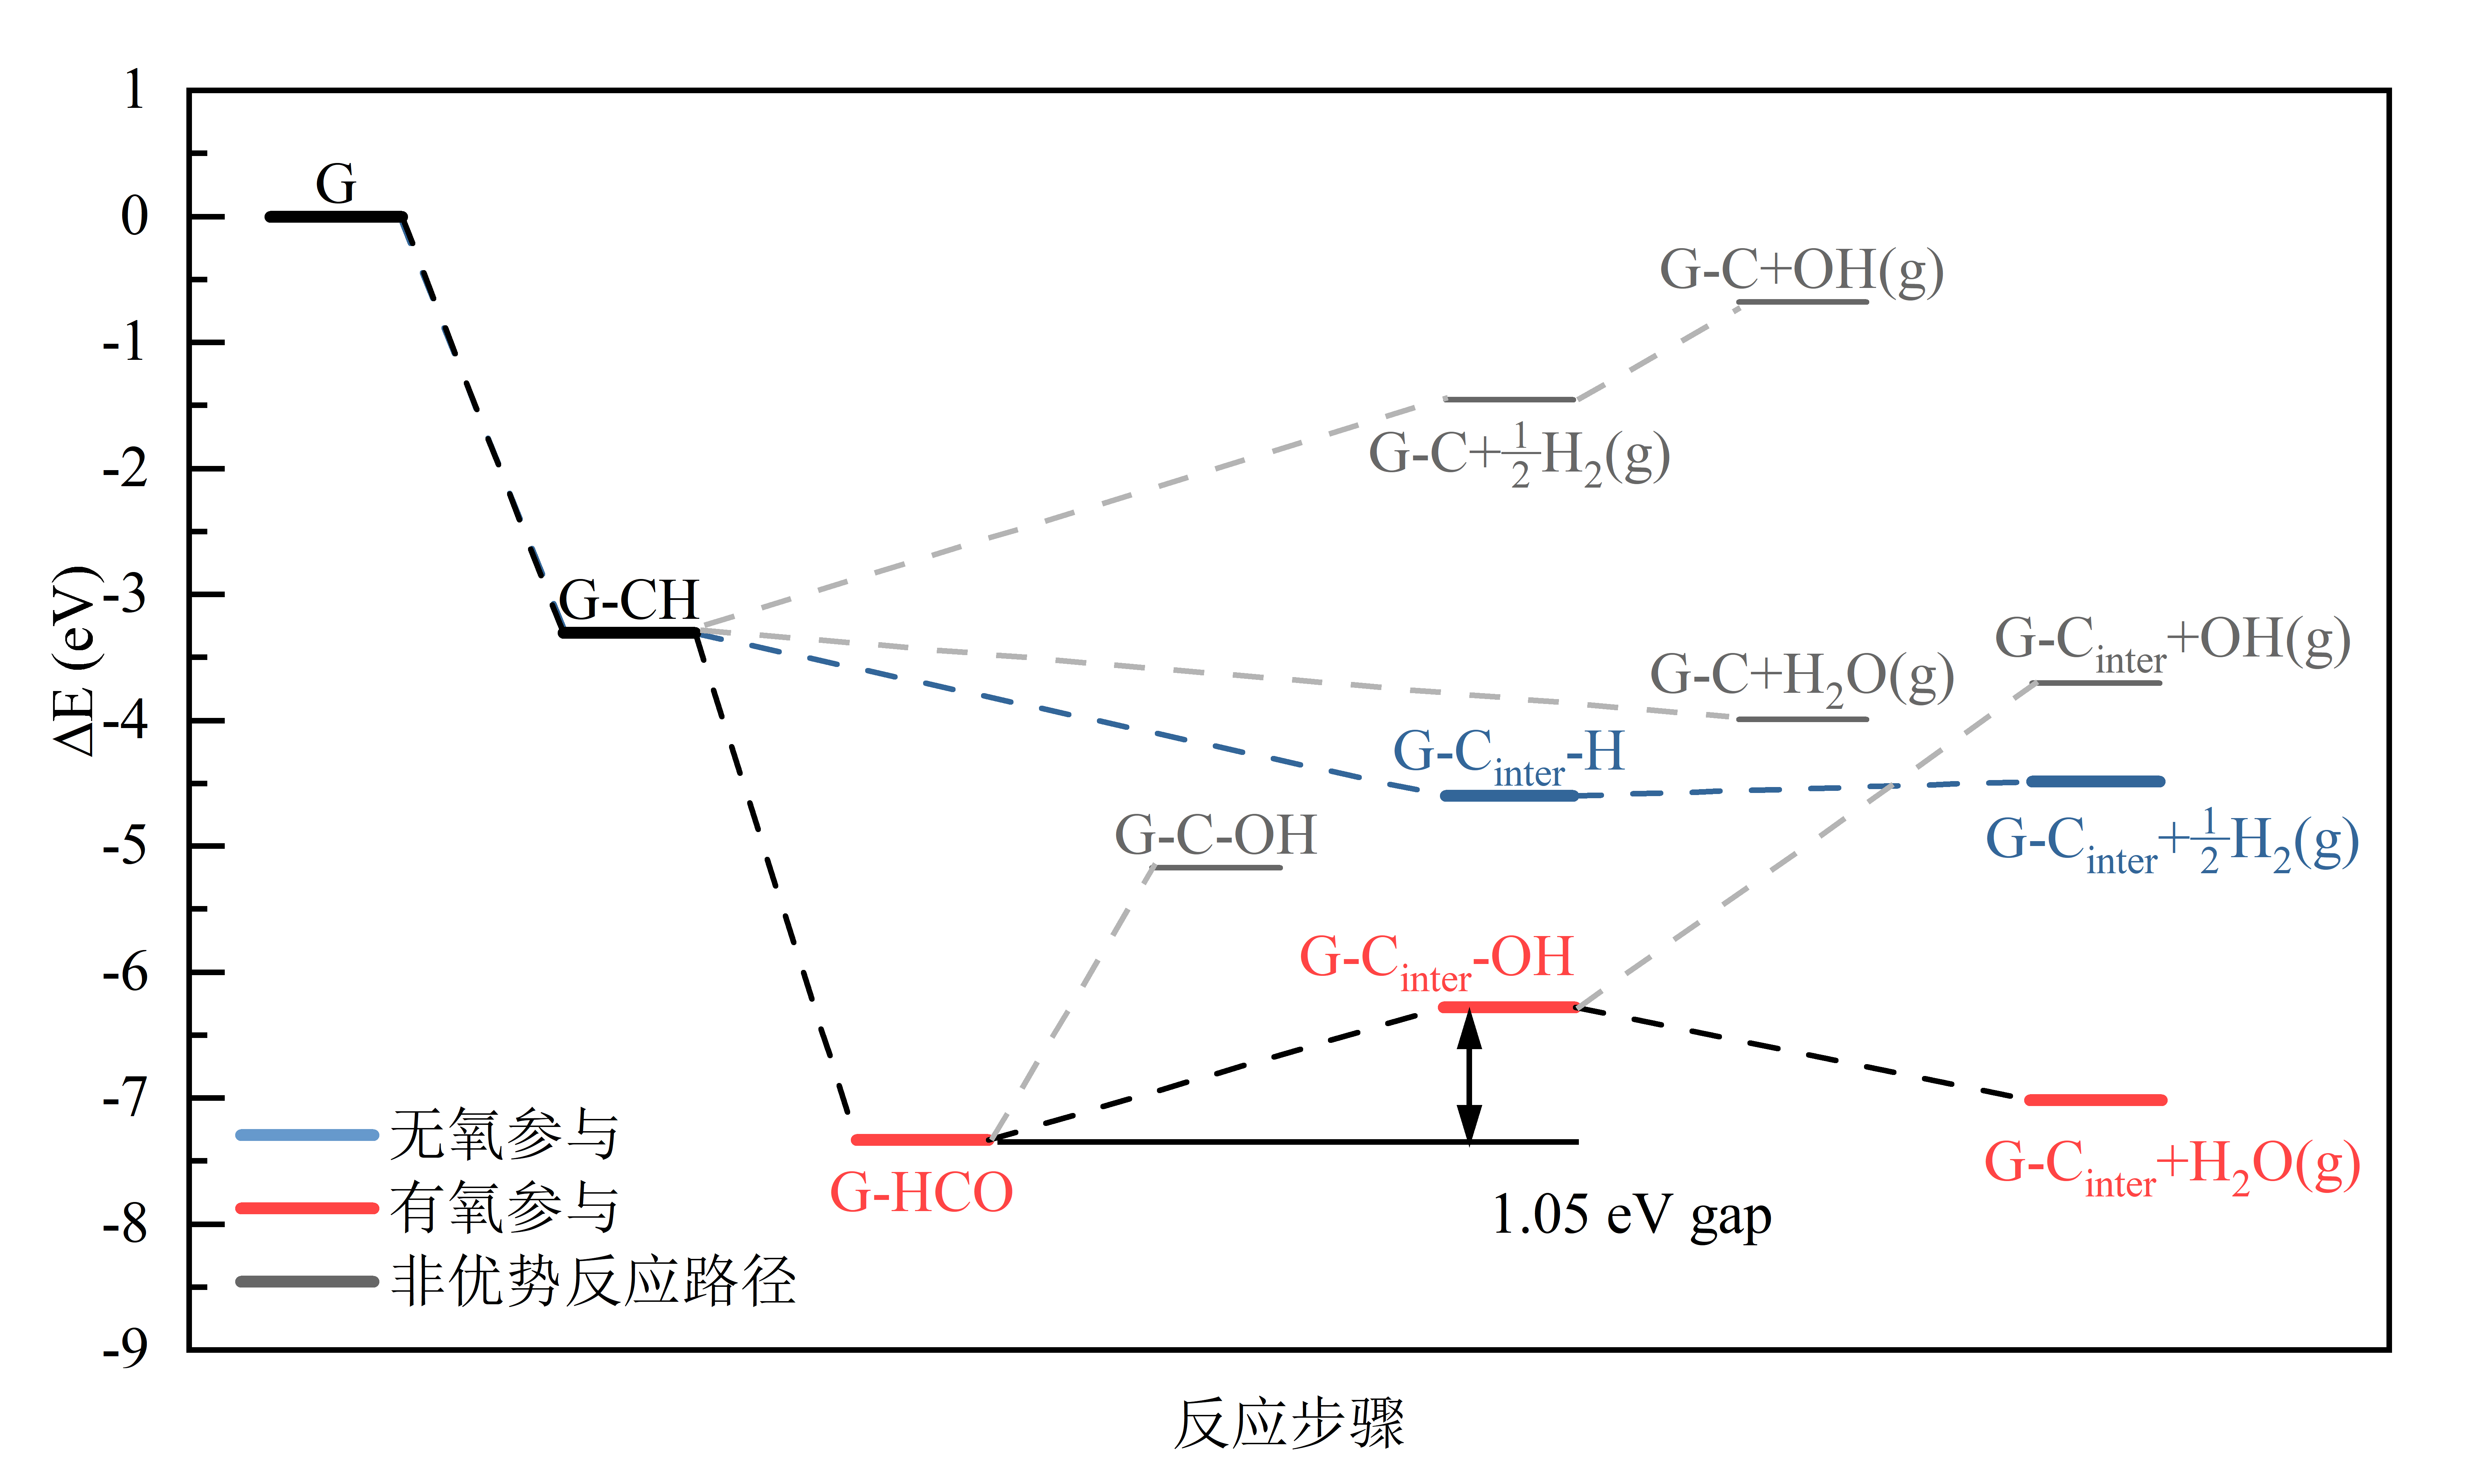
\includegraphics{pic/FLG_DFT_CHpene.png}
    \caption{含氧气氛下石墨烯表面\cemb{CH}的穿透反应过程。}
    \label{fig:FLG_DFT_CHpene}
\end{figure}

然而在有氧的情况下,在石墨烯表面吸附的\cemb{CH}会优先和氧原子结合,在石墨烯的表面形成非常稳定的\cemb{CHO}。这一反应的反应能比\cemb{CH}穿透作用的反应能低$\SI{1.03}{\electronvolt}$。氧的引入阻断了\cemb{CH}通过穿透作用生长石墨烯多层的路径,并将其变为在石墨烯表面吸附的\cemb{CHO}。而\cemb{CHO}在石墨烯表面的吸附同样也遇到了困难。计算显示由于\cemb{CHO}在石墨烯表面极高的稳定性,其进行穿透反应所需吸收的能量约为$\SI{1.05}{\electronvolt}$。即使在穿透了碳原子后,残留的\cemb{OH}官能团与气氛中的\cemb{H}反应形成水蒸气也仍旧比\cemb{CHO}在石墨烯上吸附的能量要高。

\begin{figure}[htb]
    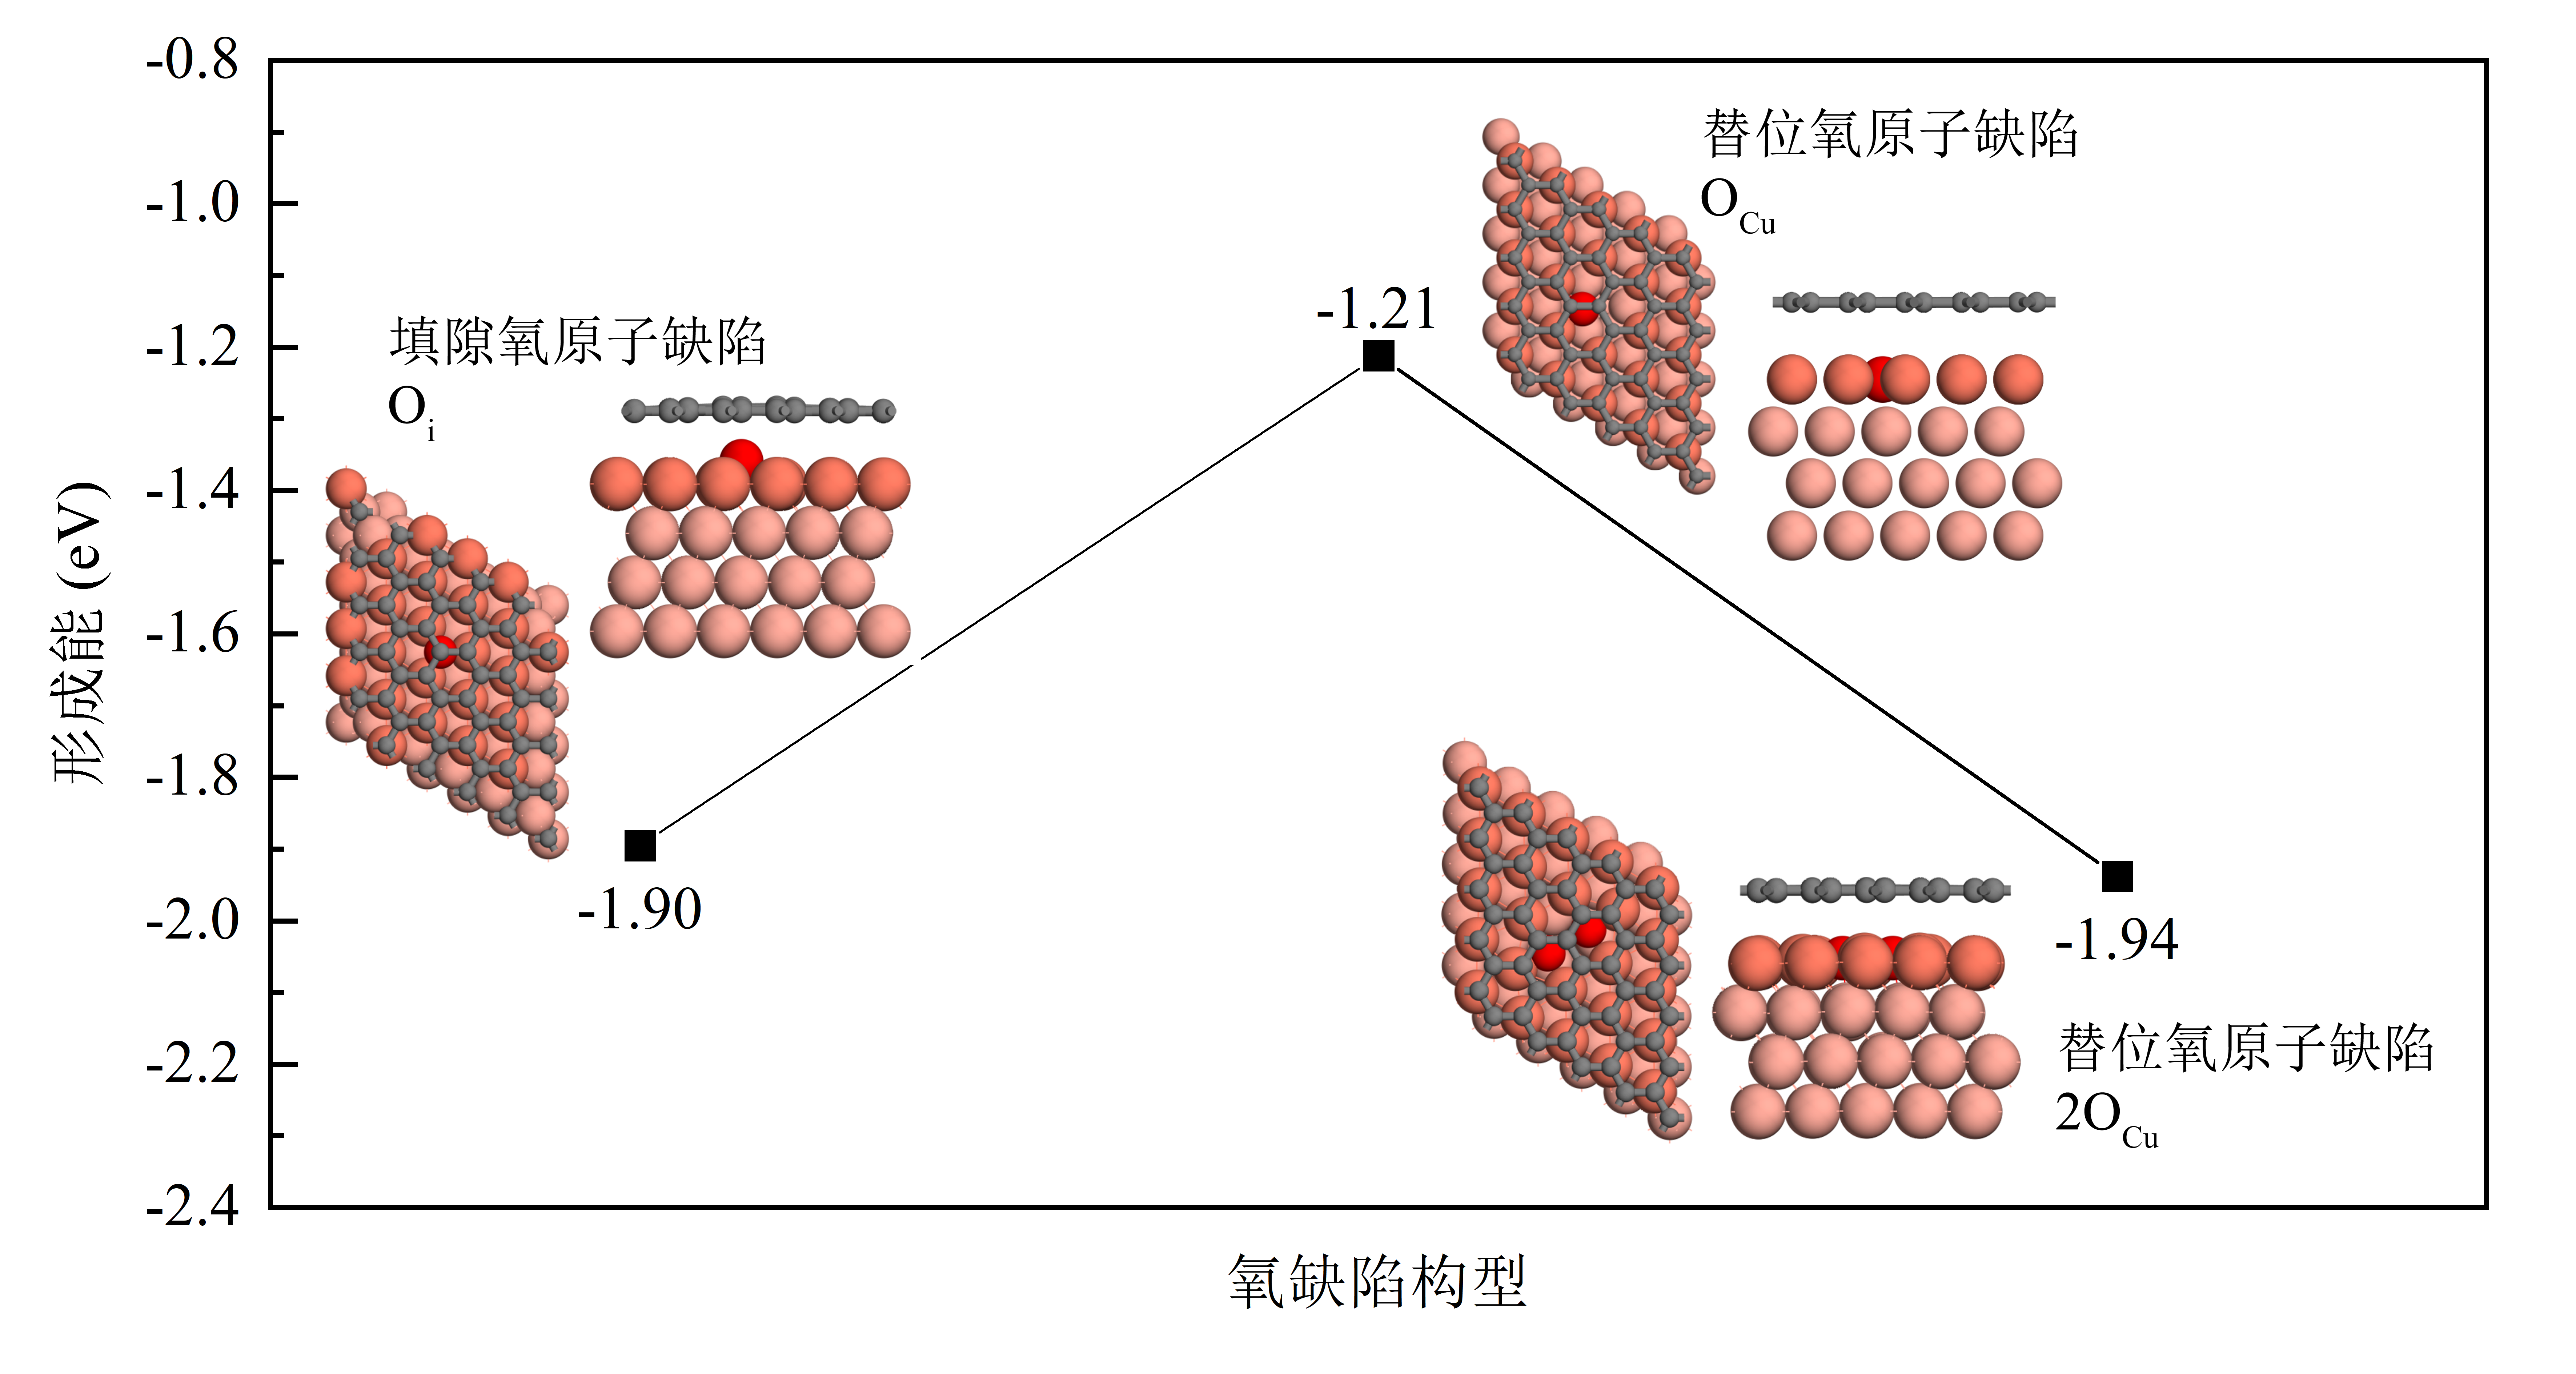
\includegraphics{pic/FLG_DFT_Odefect.png}
    \caption{铜衬底表面不同构型的氧缺陷的形成能。图中,铜原子、碳原子、氧原子、氢原子分别使用橙色、灰色、红色和白色标识。}
    \label{fig:FLG_DFT_Odefect}
\end{figure}

在含氧的生长气氛下,铜衬底可能产生氧缺陷。而铜衬底表面的氧缺陷可能会对\cemb{CHO}在石墨烯表面的穿透作用产生影响。为了简化后续计算,我们首先对不同构型的氧缺陷进行形成能计算。如图\ref{fig:FLG_DFT_Odefect}所示,我们考虑了铜衬底表面氧的三种简单的点缺陷,分别为\chinesecolon 填隙氧原子缺陷\cemb{O_{i}}、单氧原子替位缺陷\cemb{O_{Cu}}以及双氧原子替位缺陷\cemb{2O_{Cu}},其中替位缺陷均为替换单个铜原子。形成能的计算使用$E_{\rm f}=E_{\rm Cu}^{\rm defect}+{\rm n_{Cu}}E_{\rm Cu}^{\rm bulk}-\frac{1}{2}{\rm n_{O}}E_{O_{2}} - E_{\rm Cu}^{\rm perfect}$。其中$E_{\rm Cu}^{\rm defect}$和$E_{\rm Cu}^{\rm perfect}$为缺陷铜衬底和完美铜衬底的能量;$E_{\rm Cu}^{bulk}$和$E_{O_{2}}$为块体铜和氧气的能量;${\rm n_{Cu}}$和${\rm n_{O}}$为缺陷反应中涉及的铜原子和氧原子的数量。计算结果显示三种点缺陷的形成能均为负值,形成能最高的单氧原子替位缺陷\cemb{O_{Cu}}的计算值为$\SI{-1.21}{\electronvolt}$。因此,我们认为在生长了石墨烯的情况下,铜衬底的表面仍然很容易形成氧原子缺陷。计算得到的形成能最低的氧缺陷构型为双氧原子替位缺陷\cemb{2O_{Cu}},其形成能为$\SI{-1.94}{\electronvolt}$。在后续的计算中,我们使用双氧原子替位缺陷\cemb{2O_{Cu}}作为主要研究对象,考察\cemb{CHO}在石墨烯表面的穿透作用。

在图\ref{fig:FLG_DFT_CHOpene}中,我们绘制了铜衬底上不同位点的石墨烯表面吸附的\cemb{CHO}的穿透反应过程,包含无氧缺陷的原生位点以及双氧原子替位缺陷\cemb{2O_{Cu}}的氧缺陷位点。对比\cemb{CHO}在铜表面原生位点的石墨烯穿透反应,铜表面的氧缺陷位点对于游离碳有更高的亲和性,消除了\cemb{CHO}穿透石墨烯的上升势。具体而言,在铜衬底的氧缺陷位点,吸附在石墨烯表面的\cemb{CHO}的穿透反应能为$\SI{-1.27}{\electronvolt}$。同时,在穿透反应完成后,石墨烯上残留的\cemb{OH}官能团能与气氛中的氢反应,进一步降低体系能量并且释放处氧缺陷位点,使得\cemb{CHO}在氧缺陷位点的穿透反应能够持续不断的进行。虽然穿透反应过程中的交换作用使得原石墨烯单层表面的碳原子进入界面成为游离碳,但是\cemb{CHO}对于石墨烯表面的铜衬底位点选择性穿透使得在界面处生长的石墨烯多层的碳原子主要来源于含氧气氛内的碳源。倘若穿透反应能够在石墨烯单层表面的任意位点进行,那么由于石墨烯表面吸附分子的扩散作用,穿透进入界面的游离碳并成核生长为石墨烯多层点的碳原子应该主要来自于原石墨烯单层的碳原子。因为在随机作用下,只有很少的位点会产生多次穿透的现象。如果穿透反应对于铜衬底的氧缺陷位点具有选择性,氧缺陷位点处产生的穿透通道使得大部分的穿透都在氧缺陷位点上方进行,由此会产生在石墨烯单层表面多次穿透的情况,如此一来穿透进入界面的游离碳并成核生长为石墨烯多层点的碳原子则主要来源于生长气氛。因此,通过同位素标记法区别原石墨烯单层表面的碳原子以及含氧气氛中的碳原子,我们可以通过实验验证穿透的机制的选择性\citing{RN1262-2021}。
\begin{figure}[!htb]
    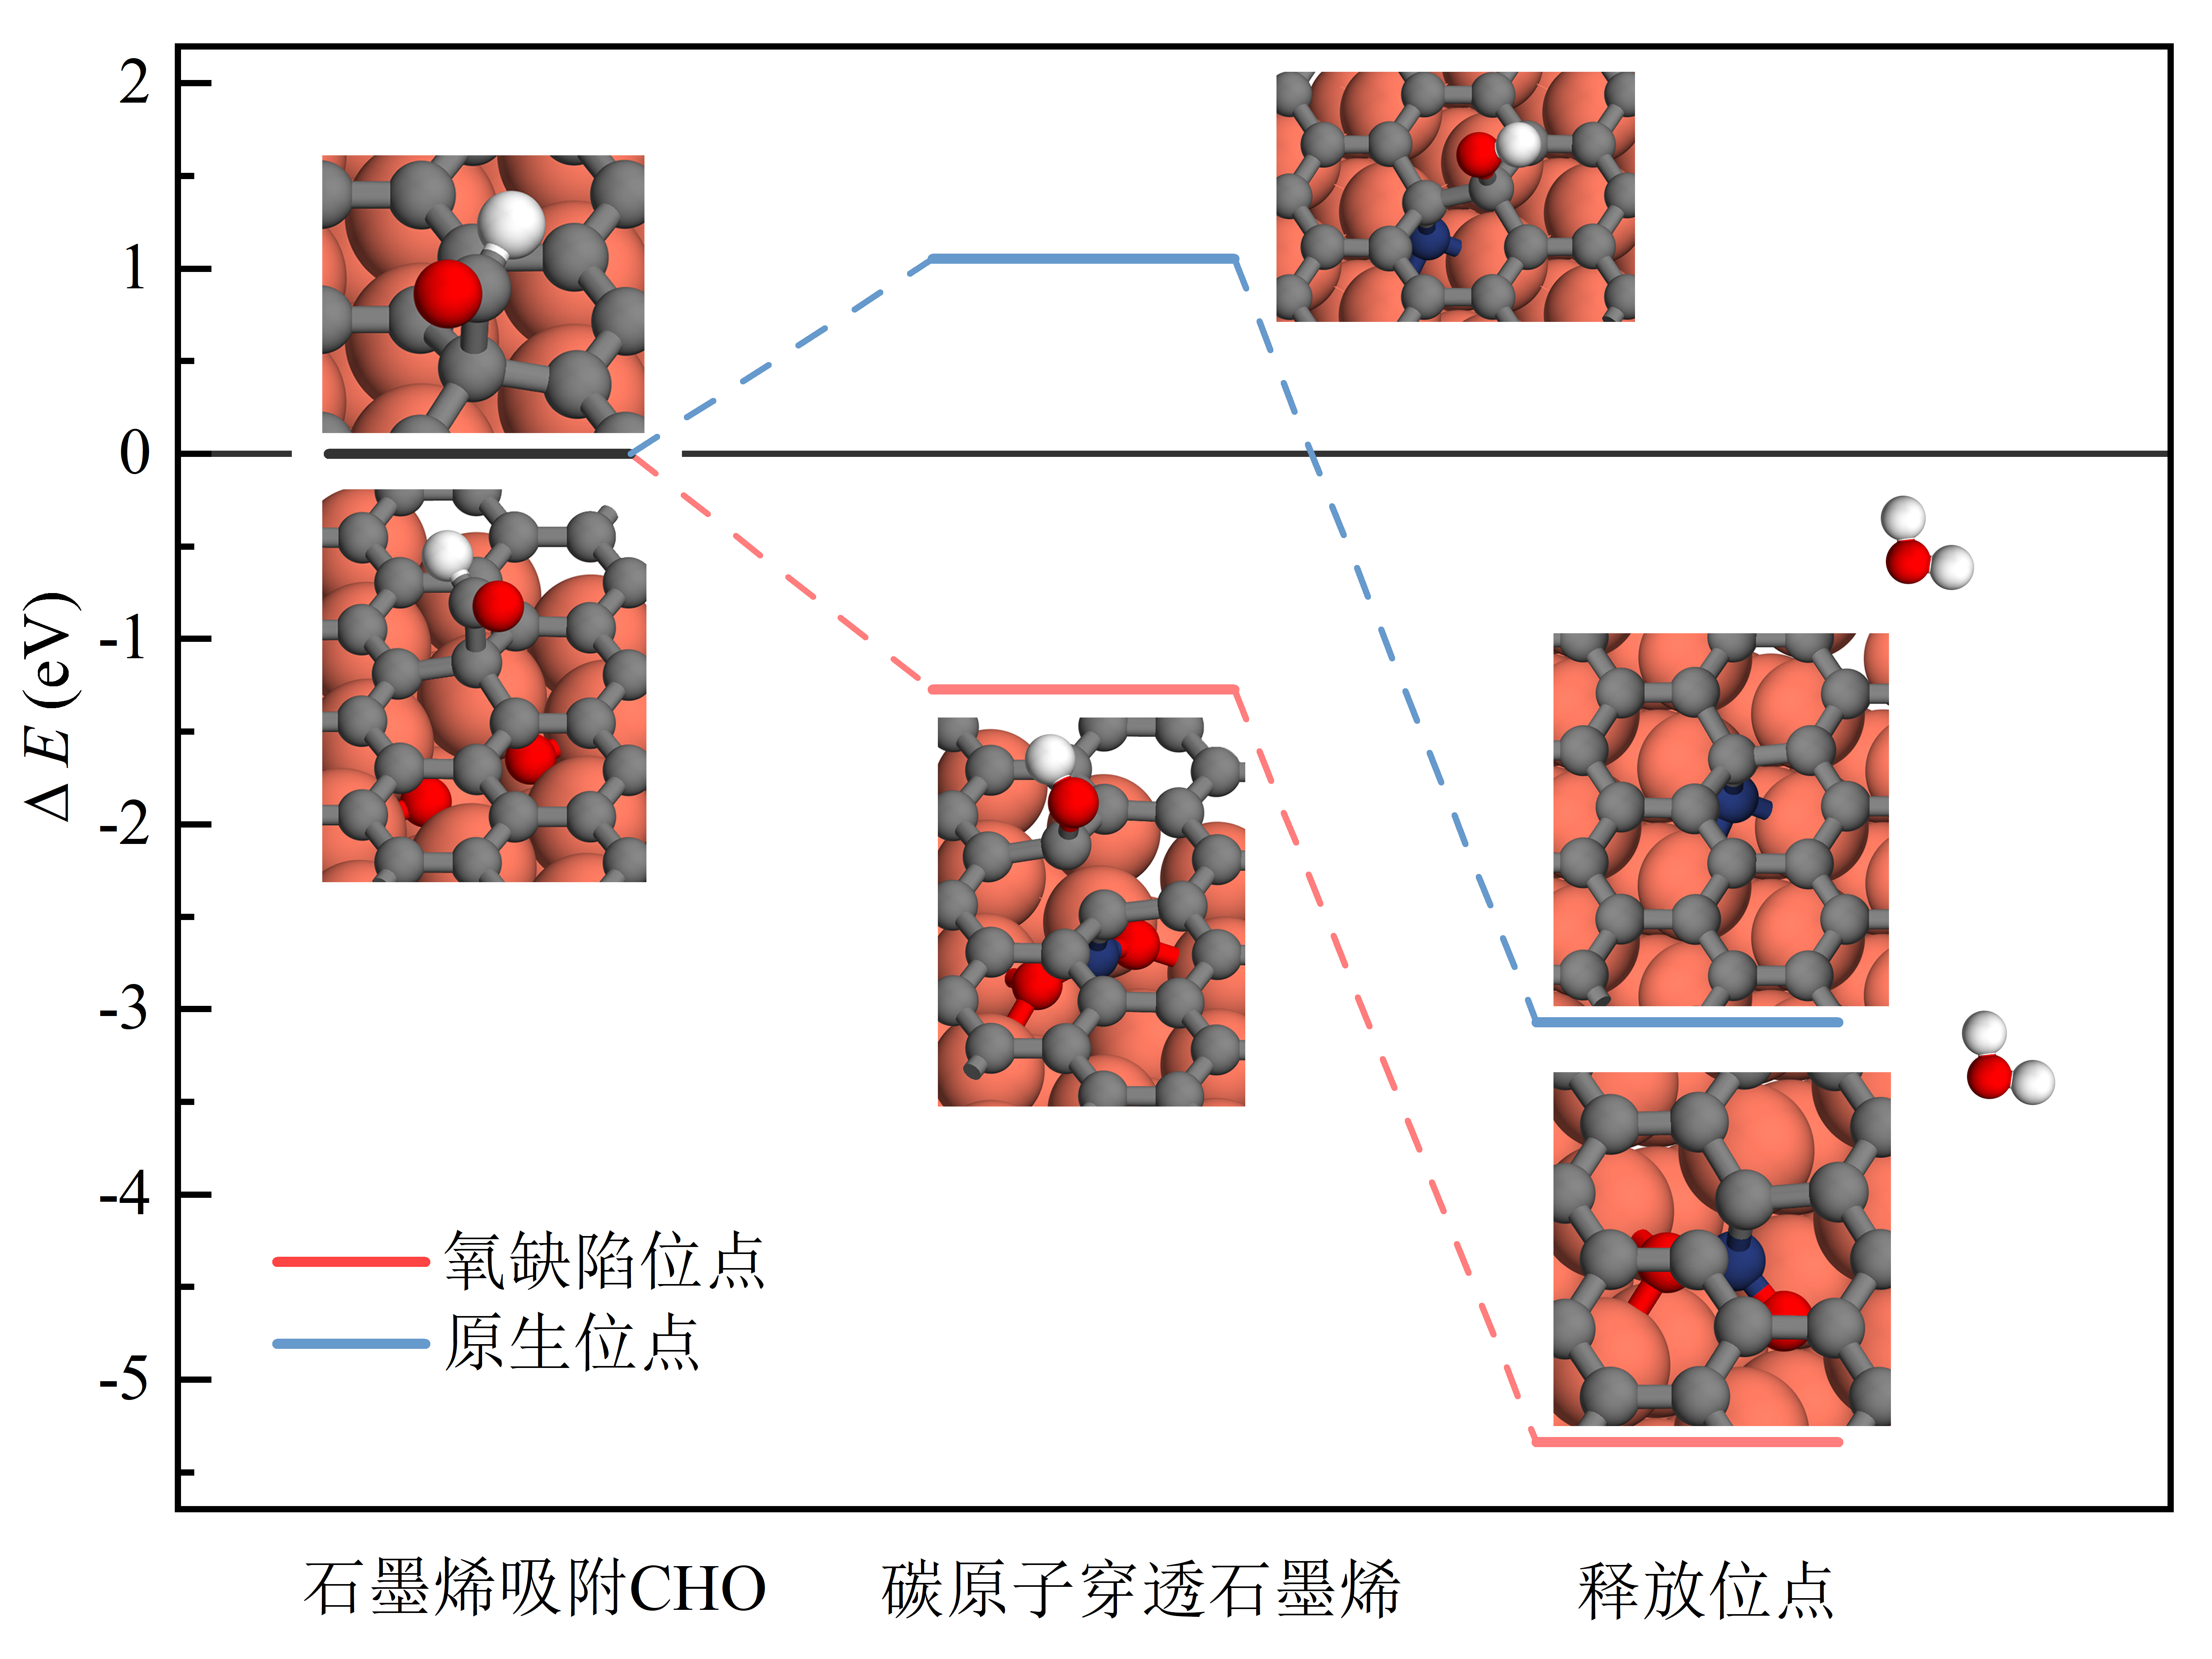
\includegraphics{pic/FLG_DFT_CHOpene.png}
    \caption{铜衬底上不同位点的石墨烯表面吸附的\cemb{CHO}的穿透反应过程。图中,铜原子、碳原子、氧原子、氢原子分别使用橙色、灰色、红色和白色标识。穿透进入界面的游离碳原子使用蓝色标识。}
    \label{fig:FLG_DFT_CHOpene}
\end{figure}

\subsection{氧辅助多层石墨烯蚀刻生长模型及模式切换相图}
综合考虑氧气的引入对于界面处石墨烯多层蚀刻和生长的影响,我们可以发现氧对二者均有促进作用。对于氧蚀刻反应,根据通入的氧流量的不同导致生长气氛中氧的化学势$\muO{}$的变化,我们将蚀刻反应分为两个阶段。在第一个阶段中,只有界面处的游离碳通过与石墨烯单层的交换左右,被气氛中的氧蚀刻,导致界面游离碳的浓度$\Cdis$下降,界面石墨烯多层点减少。第二个阶段是当通入的氧流量足够高时,氧的化学势超过蚀刻石墨烯单层的平衡化学势$\muO{} \geqslant \muO{eg}$,导致石墨烯单层开始被氧蚀刻。我们可以将氧对石墨烯的蚀刻作用总结为以下化学表达式\chinesecolon
\begin{equation}
    \label{chemeq:OetchReaction}
    \begin{split}
        \cemb{C($\rm dis.$) + O($\rm ads.$) &->[graphene] CO(g)} \\
        \cemb{C(graphene) + O($\rm ads.$) + 2H &->[\vphantom{graphene}] CO(g) } \mbox{ only if $\muO{} \geqslant \muO{eg}$}
    \end{split}
\end{equation}

根据\ref{subsec:Opene}章,氧辅助的穿透反应可以写为\chinesecolon
\begin{align}
    \label{chemeq:OpeneReaction}
    \cemb{C2H2(g) + 2O($\rm ads.$) + 2H(g) ->[graphene][Cu oxygen defect] 2C(adlayer) + H2O(g)}
\end{align}

根据反应式\ref{chemeq:OetchReaction},我们可以写出理想状况下的蚀刻速率\chinesecolon
\begin{equation}
    \RateV{e}{}=\rule[0ex]{0ex}{8ex}\left\{
        \begin{array}{ll}
        \smash[t]{\overbrace{\RateK{e}{dis.}\Cdis\Oads}^{\mathclap{{\mbox{\normalsize $\RateV{e}{dis.}$}}}}} & \mbox{}  \\
        \smash[b]{\RateK{e}{dis.}\Cdis\Oads+\RateK{e}{g}\Oads} & \mbox{for $\muO{} \geqslant \muO{eq}$} 
        \end{array}\right.
        %\begin{array}{ll}\hline
        %    \rule[10ex]{1ex}{4ex}\\\hline
        %\end{array}
\end{equation}

和穿透速率\chinesecolon
\begin{equation}
    \RateV{g}{}=\RateK{g}{}\cemb{[C2H2][H2]^2}\Oads^2
\end{equation}

其中,$\RateK{e}{dis.}$、$\RateK{e}{g}$和$\RateK{g}{}$分别为游离碳蚀刻,石墨烯单层蚀刻,石墨烯多层生长的反应常数。$\Cdis$、$\cemb{[C2H2]}$、$\cemb{[H]}$和$\Oads$代表界面游离碳、$\cemb{C2H2}$化合物、$\cemb{H}$自由基以及石墨烯上吸附氧的浓度。

考虑蚀刻石墨烯多层时,氧原子对于的界面游离碳消耗\chinesecolon
\begin{equation}
    \RateV{e}{dis.}=\RateK{e}{dis.}\left(\Cdis-\RateV{e}{dis.}\right)\Oads
\end{equation}

其中,$t$为反应的时间。随着氧原子对石墨烯多层蚀刻的进行,界面游离碳逐渐被消耗,$\Cdis$的下降同时降低了石墨烯多层蚀刻反应的速率。将反应速率$\RateV{e}{dis.}$对反应时间$\ReactTime{O}{}$积分并取平均,我们可以得到$\ReactTime{O}{}$时间段内的氧气对游离碳的平均蚀刻反应速率\chinesecolon
\begin{equation}
    \overline{\RateV{e}{dis.}}=\frac{\int_{0}^{\ReactTime{O}{}} \RateV{e}{dis.} \,dt }{\ReactTime{O}{}}=\frac{\int_{0}^{\ReactTime{O}{}} \frac{\RateK{e}{dis.}\Cdis\Oads}{\RateK{e}{dis.}\Oads \ReactTime{}{} + 1} \,dt}{\ReactTime{O}{}}
\end{equation}

而对于生长反应,$\cemb{CHO}$在石墨烯表面的选择性吸附使得生长反应速率$\RateV{g}{}$存在一个由铜衬底表面氧缺陷位点数量限制的上界。我们可以写出在氧缺陷处的穿透通道被饱和之前的生长反应的平均速率\chinesecolon
\begin{equation}
    \overline{\RateV{g}{}}=\frac{\int_{0}^{\ReactTime{O}{}} \RateV{g}{} \,dt }{\ReactTime{O}{}}= \frac{\int_{0}^{\ReactTime{O}{}} \RateK{g}{}\cemb{[C2H2][H2]^2}\Oads^2 \,dt }{\ReactTime{O}{}}
\end{equation}

在这些化合物的浓度中,$\cemb{[C2H2]}$和$\cemb{[H]}$我们使用\ref{subsec:FLG_gasPhase}节中模拟出的相应化合物的稳态浓度数据。而对于$Odis$,虽然在\ref{subsec:FLG_gasPhase}章中的模拟证明生长环境中的化合物很快就达到了稳态平衡,但由于氧自由基($\cemb{O}$)较低的浓度以及氧分子($\cemb{O2}$)在石墨烯表面较高的吸附能。氧气的吸附过程可能会需要很长的一段时间才会达到饱和。为了获得$\Oads$在石墨烯多层生长过程中随时间的变化情况,我们使用晶格随机顺序吸附模型(lattice random sequential adsorption model )对氧气以及氧原子在石墨烯表面的吸附进行模拟。

晶格随机顺序吸附模型中,我们使用二维晶格对石墨烯进行模拟,每个晶格单元对应一个原胞大小的石墨烯。在模拟过程中,我们考虑生长气氛中氧气分子($\cemb{O2}$)和氧自由基($\cemb{O}$)在石墨烯表面的沉积。根据密度泛函理论计算(表\ref{tab:FLG_RSA_coverage}),取$\cemb{O2}$和$\cemb{O}$在石墨烯表面吸附的饱和覆盖率分别为$1$和$1 / 4$。

\begin{table}
    \centering
    \caption{}
    \begin{tabular}{ccc}
        \toprule
        覆盖率  & $\cemb{O}$的吸附能(\si{\electronvolt}) & $\cemb{O2}$的吸附能(\si{\electronvolt}) \\
        \midrule
        1       & -4.50                                    & 0.43                                      \\
        $1 / 4$ & -4.95                                    & -0.026                                    \\
        \bottomrule
    \end{tabular}
    \label{tab:FLG_RSA_coverage}
\end{table}

同时,有别于氧自由基($\cemb{O}$)的直接吸附,氧气分子$\cemb{O2}$在石墨烯上的吸附的同时需要较高的能量进行进行裂解。我们通过在氧气分子吸附的过程中添加$\SI{2.39}{\electronvolt}$的势垒来对这个裂解过程进行描述\citing{RN838-2012}。为了将随机吸附模拟过程中的模拟时间时长与实际通入氩氧混合气的时长进行对应,我们根据气体的麦克斯韦-玻尔兹曼分布计算了氧自由基($\cemb{O}$)和氧气分子$\cemb{O2}$的碰撞频率,气氛中氧自由基($\cemb{O}$)和氧气分子$\cemb{O2}$的浓度也根据\ref{subsec:FLG_gasPhase}节中的模拟数据进行计算。

在图\ref{fig:FLG_RSA_Oadsorb}中,我们计算了通入不同流量的氩氧混合气的情况下石墨烯上吸附的氧原子浓度$\Oads$随时间的变化情况。计算结果显示模拟得出的$\Oads$服从指数增长定律$\Oads\left(\it t\right)=\Oads\left(\it \infty \right)-\it De^{\it -\sigma t}$,和先前的研究一致\citing{RN837-1990,RN836-1991}。由于$\Oads$的指数形式,直接将$\Oads$带入计算$\overline{\RateV{e}{dis.}}$中的积分项为非初等函数。考虑到在实际的化学气相沉积生长过程中,氧原子在低浓度氧环境中需要花费数天甚至一个月的时间才能达到饱和吸附,远超我们所考虑的生长时间范畴。而高浓度氧环境中会导致石墨烯被完全蚀刻,也不在我们所关心的范围内。因此我们将研究范围集中在氧原子吸附浓度$\Oads$的线性吸附区,这时$\Oads$相对于时间的变化关系可以简化为$\Oads\left(\it t\right)\approx \it D \sigma t$。

\begin{figure}[htb]
    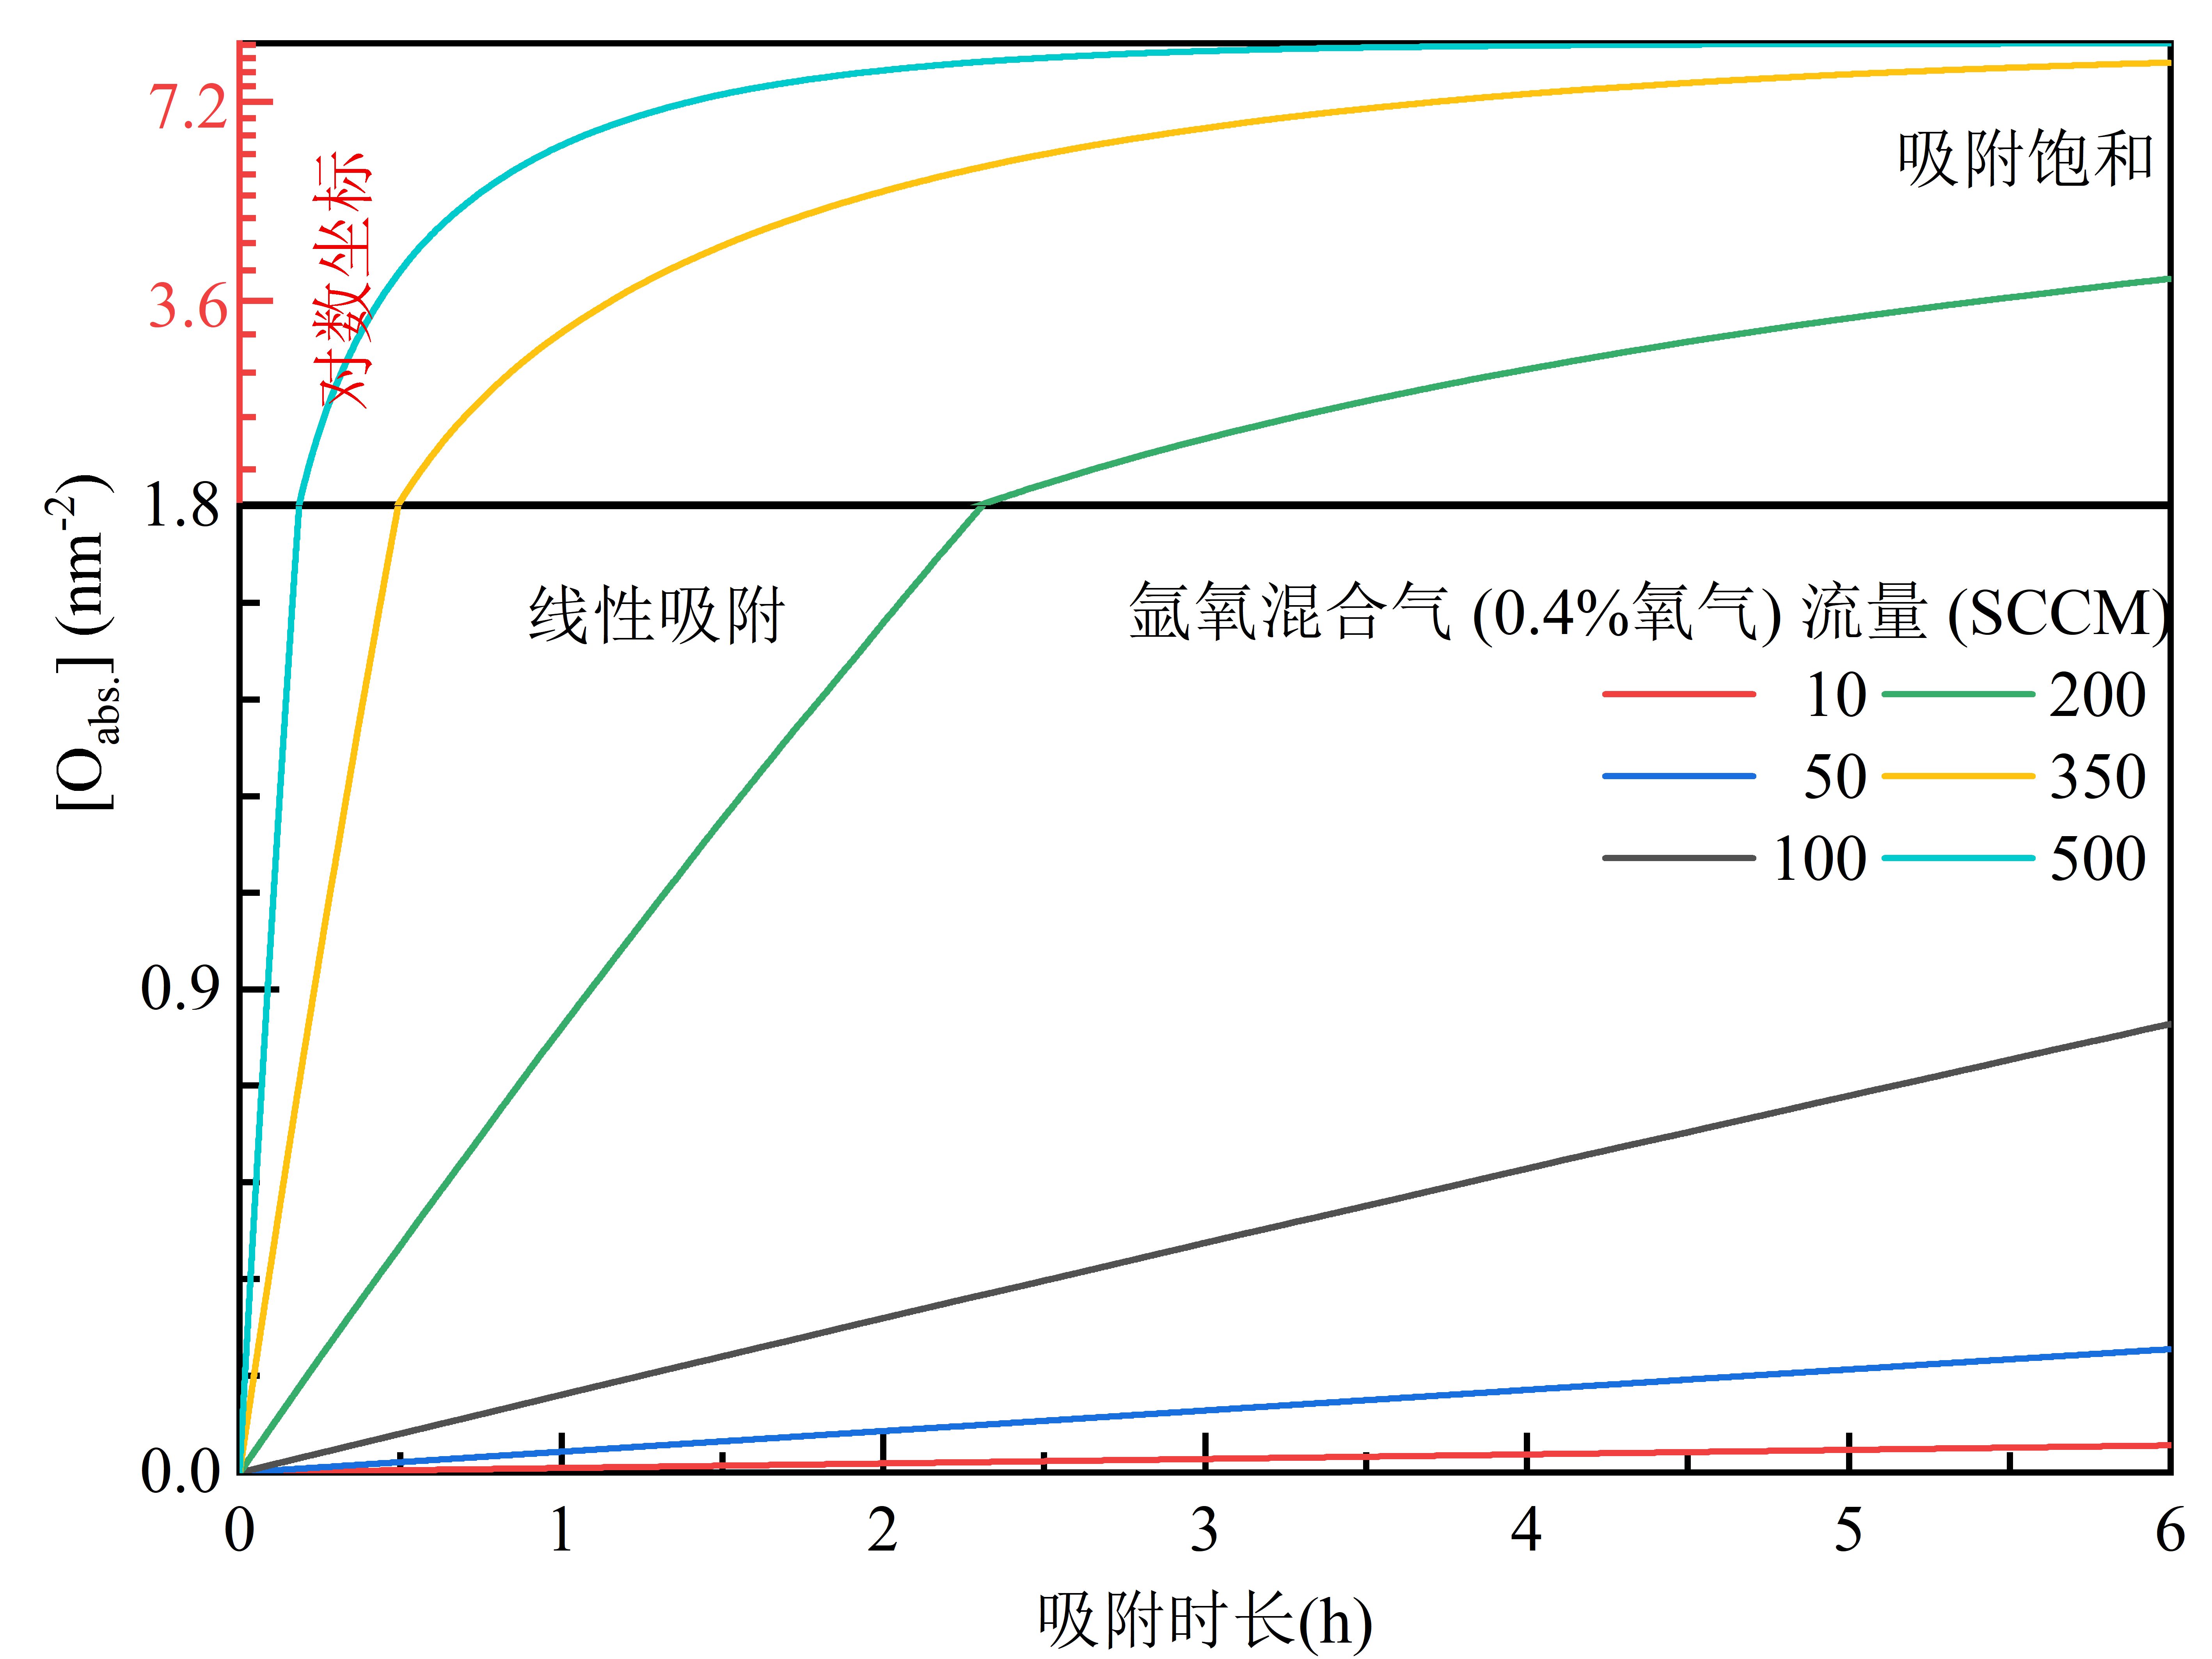
\includegraphics{pic/FLG_RSA_Oadsorb.png}
    \caption{不同氩氧混合气通入流量下氧原子在石墨烯表面吸附浓度随时间的变化情况。}
    \label{fig:FLG_RSA_Oadsorb}
\end{figure}

为了确认$\Oads$线性简化是否会因为晶格随机顺序吸附模拟过程中所使用的的屏蔽系数参数的变动而失效。如图\ref{fig:FLG_RSA_OabsorbPera}所示,我们计算了在中等氧通量的情况下(氩氧混合气流量为\SI{100}{SCCM}),多种模拟参数组合下氧原子在石墨烯表面进行吸附模拟的结果。可以看到,氧气$\cemb{O2}$屏蔽系数的变化几乎无法传到至最后吸附浓度的变化。这可能是由于氧气较高的解离势垒导致尽管生长气氛中的氧气浓度较高,但氧气在石墨烯表面解离吸附在石墨烯上的能力仍然较弱。而对于氧自由基$\cemb{O}$,屏蔽系数由$1$变为$\frac{1}{2}$会降低吸附氧原子的浓度。但考虑到通常化学气相沉积法对石墨烯的生长过程通常在$\SI{10}{\hour}$以内\citing{RN1262-2021}。在这个时间范围之内,氧自由基$\cemb{O}$屏蔽系数的变化对吸附氧原子浓度的影响较小。同时也并不会影响吸附氧原子浓度在$\SI{10}{\hour}$之内随时间的线性增长关系。因此,我们认为对氧原子吸附浓度$\Oads$使用$\Oads\left(\it t\right)\approx \it D \sigma t$进行简化并不会受模拟过程中屏蔽系数参数选取的影响。

\begin{figure}[htb]
    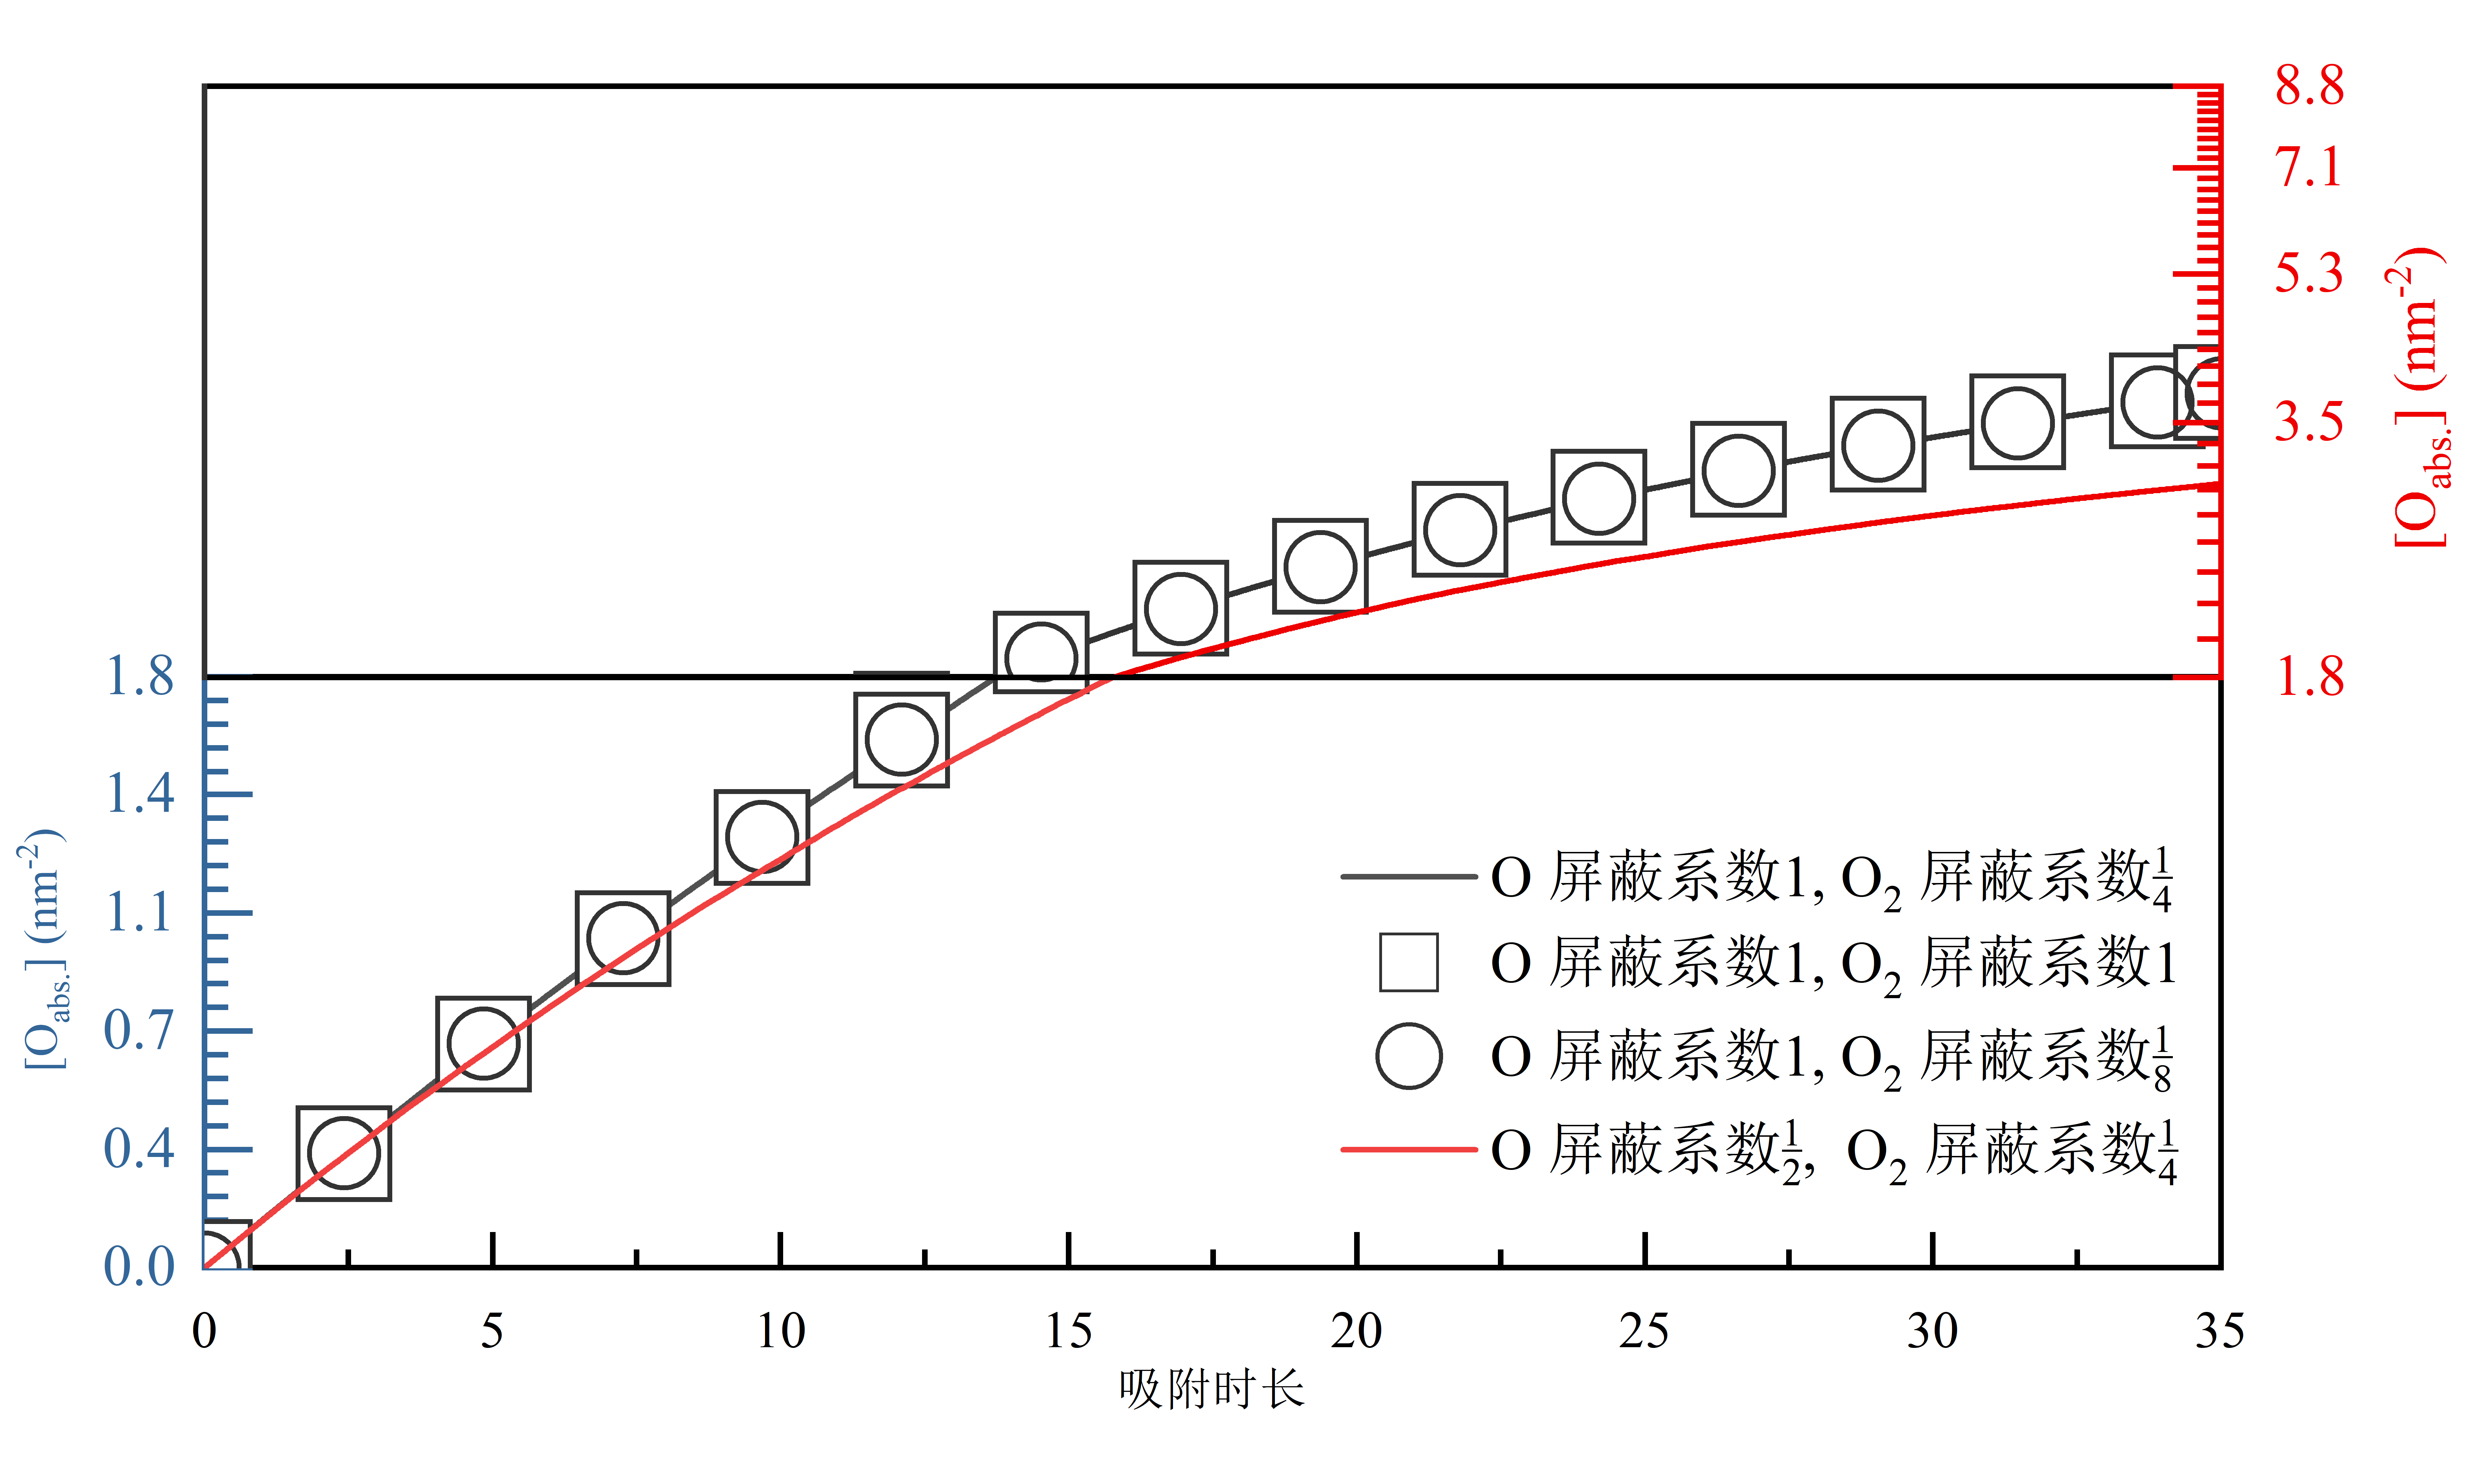
\includegraphics{pic/FLG_RSA_OabsorbPera.png}
    \caption{$\Oads\left(\it t\right)\approx \it D \sigma t$线性近似的晶格随机顺序吸附模拟参数稳定性测试}
    \label{fig:FLG_RSA_OabsorbPera}
\end{figure}

由此,我们可以计算通入$\ReactTime{O}{}$的氩氧混合气后,石墨烯的蚀刻平均速率为\chinesecolon
\begin{equation}
    \label{eq:FLG_avgVe}
    \overline{\RateV{e}{}}=
    \begin{cases}
        \frac{\Cdis_0 log\left( 1+\RateK{e}{dis.}\Oads | \,_{t=\ReactTime{O}{}} \ReactTime{O}{} \right) }{\it 2 \ReactTime{O}{}}                                                        & \muO{} < \muO{eg}         \\
        \frac{\Cdis_0 log\left( 1+\RateK{e}{dis.}\Oads | \,_{t=\ReactTime{O}{}} \ReactTime{O}{} \right) }{\it 2 \ReactTime{O}{}} + \frac{1}{2}\RateK{e}{g}\Oads| \,_{t=\ReactTime{O}{}} & \muO{} \geqslant \muO{eg}
    \end{cases}
\end{equation}

其中,界面游离碳的初始浓度$\Cdis_0$我们取相应生长温度下碳的饱和蒸汽进行近似。$\Oads| \,_{t=\ReactTime{O}{}}$为氩氧混合气的时间为$\ReactTime{O}{}$时的石墨烯上的吸附氧原子浓度。

同样,我们也可以求得在铜衬底氧缺陷产生的穿透通道饱和前,石墨烯的生长平均速率为\chinesecolon
\begin{equation}
    \label{eq:FLG_avgVg}
    \overline{\RateV{g}{}} =\frac{1}{3}\RateK{g}{}\cemb{[C2H2]}\cemb{[H]^2}\left(\Oads |_{\,\ReactTime{}{}=\ReactTime{O}{}} \right)
\end{equation}

式\ref{eq:FLG_avgVe}和式\ref{eq:FLG_avgVg}可以解释氧促石墨烯多层蚀刻和氧促石墨烯生长之间的反应速率的竞争对于石墨烯多层整体蚀刻、生长行为的影响。在图\ref{fig:FLG_model_avgV}中,我们绘制了不同吸附氧原子浓度下,氧辅助石墨烯蚀刻、生长作用的平均反应速率。

\begin{figure}[htb]
    \subfloat[]{
        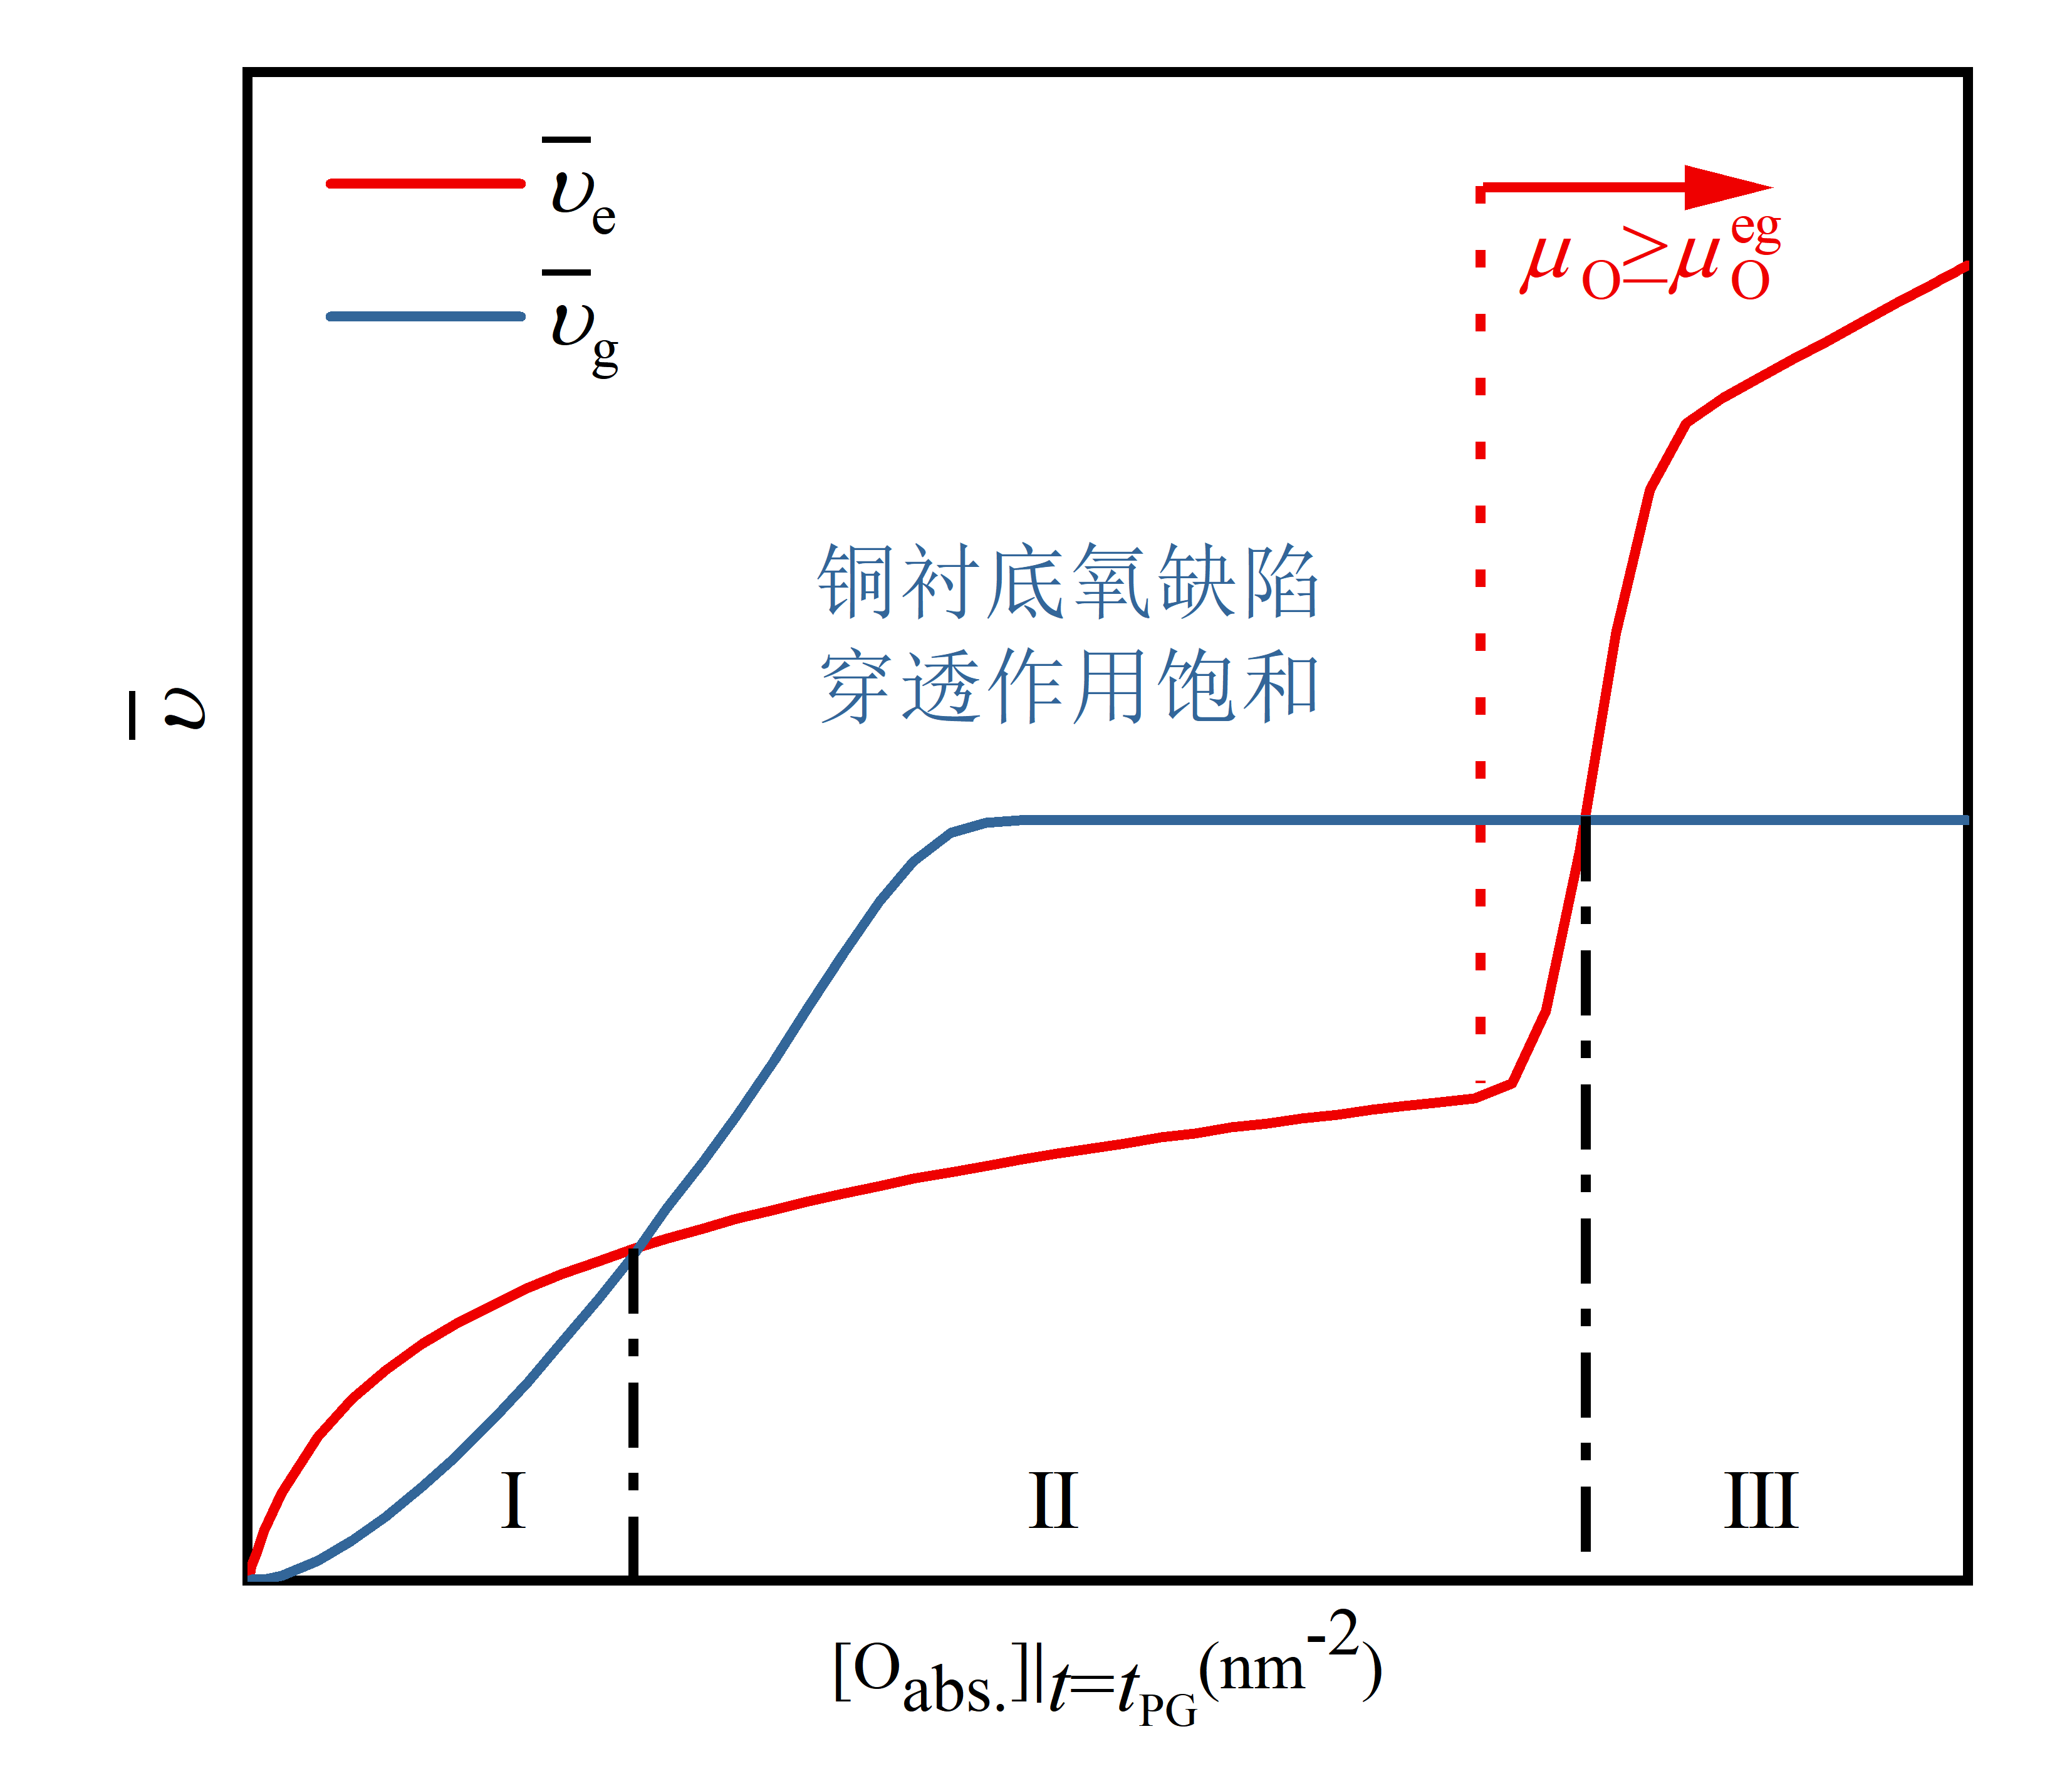
\includegraphics[]{pic/FLG_model_avgV.png}
        \label{fig:FLG_model_avgV}
    }
    \subfloat[]{
        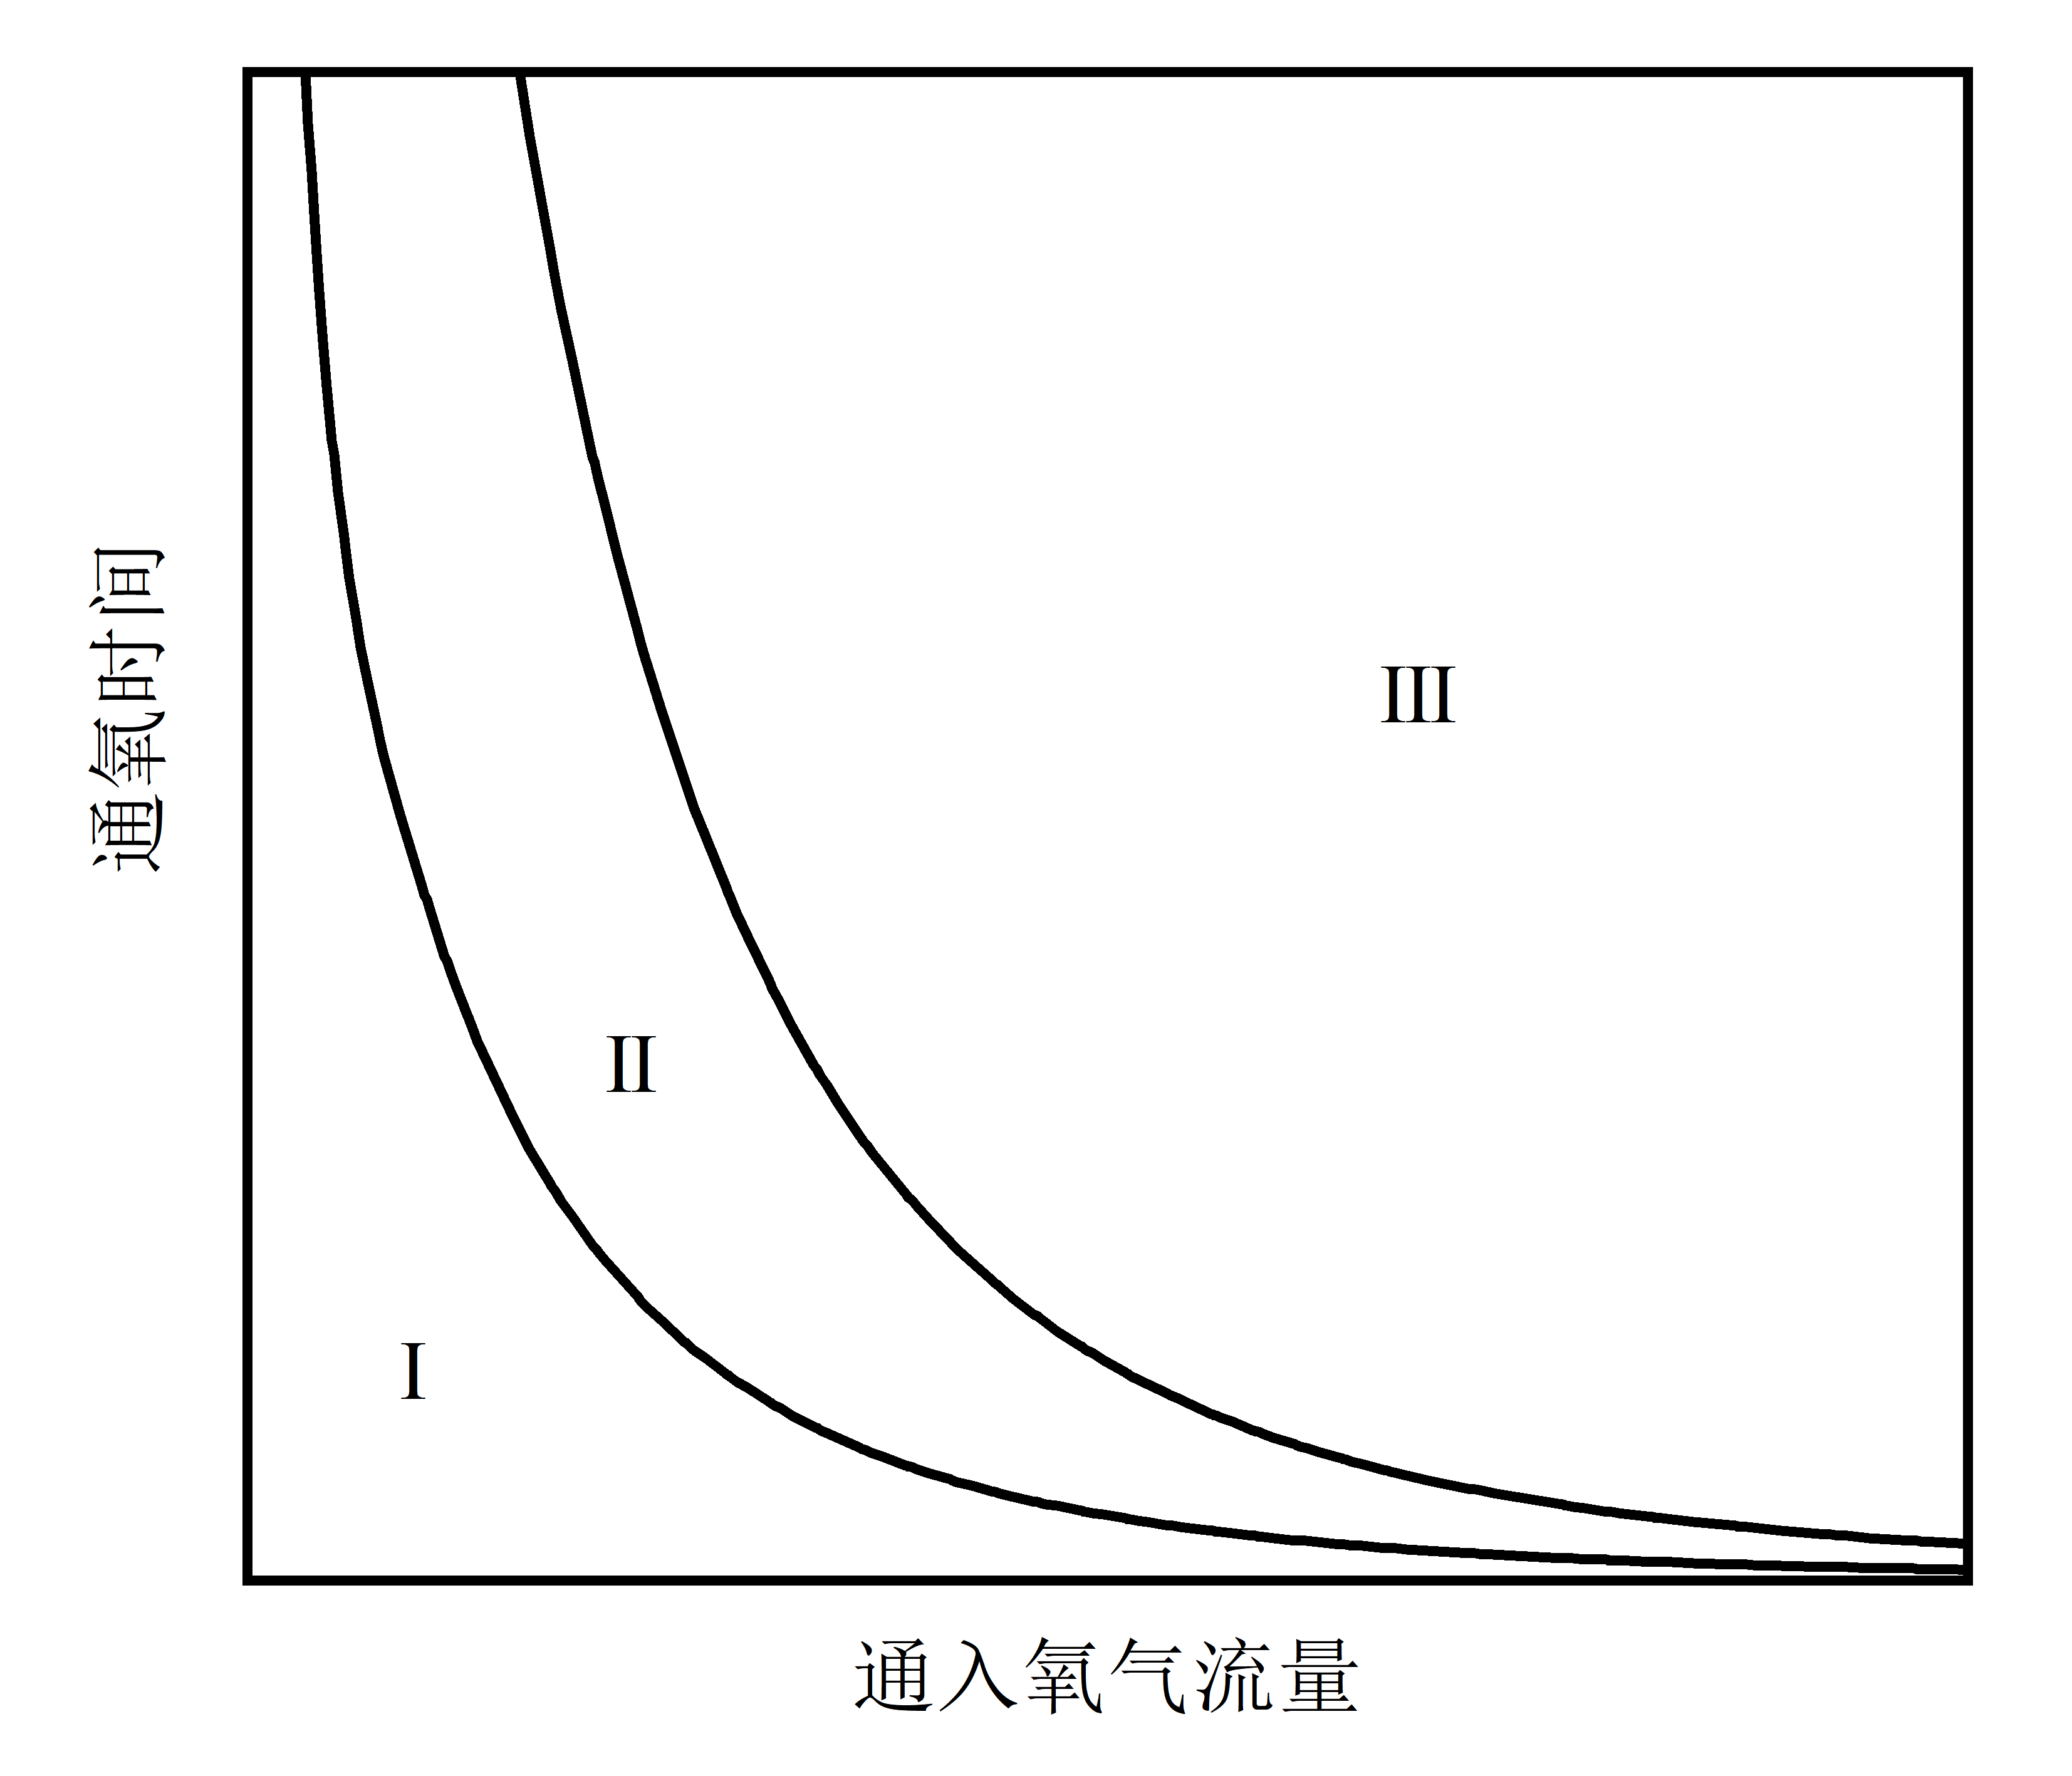
\includegraphics[]{pic/FLG_model_modePhase.png}
        \label{fig:FLG_model_modePhase}
    }
    \caption{氧辅助石墨烯蚀刻、生长作用及模式切换相图。(a)氧辅助石墨烯蚀刻、生长作用的平均反应速率;(b)氧辅助石墨烯蚀刻/生长模式切换相图。其中,模式I为石墨烯多层蚀刻、模式II为石墨烯多层生长、模式III为石墨烯蚀刻(包括石墨烯多层以及石墨烯单层)}
    \label{fig:FLG_model}
\end{figure}

图中的原点代表无氧气输入的情况,此时的石墨烯呈现出自限制的生长行为。当氧气引入生长气氛时,石墨烯表面吸附的氧原子浓度$\Oads$随着氧气通入量或者含氧气氛内反应时间的上升而上升。当吸附氧原子浓度$\Oads$较低时,石墨烯多层的蚀刻速率高于石墨烯多层的生长速率,石墨烯自限制生长下的少量多层点在氧原子的蚀刻作用下逐渐减少,整体表现出石墨烯多层蚀刻的行为(模式I)。当石墨烯表面吸附氧原子的浓度$\Oads$逐渐上升时,氧原子对于石墨烯表面的蚀刻反应速率由于界面游离碳浓度$\Cdis$的下降而放缓,$\cemb{CHO}$的穿透生长反应则随着$\Oads$的上升而继续加速。此时上升的$\Oads$导致石墨烯多层的生长速率高于被界面游离碳浓度不足所限制的的石墨烯多层蚀刻速率,整体展现出石墨烯多层生长的行为(模式II)。当$\Oads$的浓度上升至氧的化学势$\muO{}$超过蚀刻石墨烯单层的平衡化学势$\muO{eg}$,气氛中的氧开始直接蚀刻单层石墨烯,导致石墨烯蚀刻反应的速率大幅上升,再次超过被穿透通道饱和所限制的石墨烯多层生长速率。此时石墨烯展现出再蚀刻的的行为(模式III)。在模式III中,由于较高的氧活性,不仅石墨烯多层,较为稳定的石墨烯单层也会被高反应活性的氧反应。

\section{本章小结}
在本章中,我们利用理论计算的方法研究了化学气相沉积生长石墨烯过程中衬底形貌和生长气氛对于的石墨烯生长行为的影响。我们的研究表明衬底表面的台阶破坏了原衬底表面的对称性,为石墨烯的成核生长提供了优先生长位点和优先生长方向,使得石墨烯有机会在多晶铜的表面实现多点定向成核生长,有利于实现大面积石墨烯单晶生长的实现。而对于生长气氛的影响,我们的研究显示氧的引入同时促进了石墨烯多层蚀刻和多层生长的反应。而氧气对石墨烯多层的蚀刻和穿透作用的相互竞争突破了原有铜衬底上石墨烯生长的自限制作用,导致了石墨烯多层交替出现蚀刻和生长的现象,有利于实现石墨烯生长过程中的层数调控。
